\documentclass[twoside]{book}

% Packages required by doxygen
\usepackage{fixltx2e}
\usepackage{calc}
\usepackage{doxygen}
\usepackage[export]{adjustbox} % also loads graphicx
\usepackage{graphicx}
\usepackage[utf8]{inputenc}
\usepackage{makeidx}
\usepackage{multicol}
\usepackage{multirow}
\PassOptionsToPackage{warn}{textcomp}
\usepackage{textcomp}
\usepackage[nointegrals]{wasysym}
\usepackage[table]{xcolor}

% Font selection
\usepackage[T1]{fontenc}
\usepackage[scaled=.90]{helvet}
\usepackage{courier}
\usepackage{amssymb}
\usepackage{sectsty}
\renewcommand{\familydefault}{\sfdefault}
\allsectionsfont{%
  \fontseries{bc}\selectfont%
  \color{darkgray}%
}
\renewcommand{\DoxyLabelFont}{%
  \fontseries{bc}\selectfont%
  \color{darkgray}%
}
\newcommand{\+}{\discretionary{\mbox{\scriptsize$\hookleftarrow$}}{}{}}

% Page & text layout
\usepackage{geometry}
\geometry{%
  a4paper,%
  top=2.5cm,%
  bottom=2.5cm,%
  left=2.5cm,%
  right=2.5cm%
}
\tolerance=750
\hfuzz=15pt
\hbadness=750
\setlength{\emergencystretch}{15pt}
\setlength{\parindent}{0cm}
\setlength{\parskip}{3ex plus 2ex minus 2ex}
\makeatletter
\renewcommand{\paragraph}{%
  \@startsection{paragraph}{4}{0ex}{-1.0ex}{1.0ex}{%
    \normalfont\normalsize\bfseries\SS@parafont%
  }%
}
\renewcommand{\subparagraph}{%
  \@startsection{subparagraph}{5}{0ex}{-1.0ex}{1.0ex}{%
    \normalfont\normalsize\bfseries\SS@subparafont%
  }%
}
\makeatother

% Headers & footers
\usepackage{fancyhdr}
\pagestyle{fancyplain}
\fancyhead[LE]{\fancyplain{}{\bfseries\thepage}}
\fancyhead[CE]{\fancyplain{}{}}
\fancyhead[RE]{\fancyplain{}{\bfseries\leftmark}}
\fancyhead[LO]{\fancyplain{}{\bfseries\rightmark}}
\fancyhead[CO]{\fancyplain{}{}}
\fancyhead[RO]{\fancyplain{}{\bfseries\thepage}}
\fancyfoot[LE]{\fancyplain{}{}}
\fancyfoot[CE]{\fancyplain{}{}}
\fancyfoot[RE]{\fancyplain{}{\bfseries\scriptsize Generated by Doxygen }}
\fancyfoot[LO]{\fancyplain{}{\bfseries\scriptsize Generated by Doxygen }}
\fancyfoot[CO]{\fancyplain{}{}}
\fancyfoot[RO]{\fancyplain{}{}}
\renewcommand{\footrulewidth}{0.4pt}
\renewcommand{\chaptermark}[1]{%
  \markboth{#1}{}%
}
\renewcommand{\sectionmark}[1]{%
  \markright{\thesection\ #1}%
}

% Indices & bibliography
\usepackage{natbib}
\usepackage[titles]{tocloft}
\setcounter{tocdepth}{3}
\setcounter{secnumdepth}{5}
\makeindex

% Hyperlinks (required, but should be loaded last)
\usepackage{ifpdf}
\ifpdf
  \usepackage[pdftex,pagebackref=true]{hyperref}
\else
  \usepackage[ps2pdf,pagebackref=true]{hyperref}
\fi
\hypersetup{%
  colorlinks=true,%
  linkcolor=blue,%
  citecolor=blue,%
  unicode%
}

% Custom commands
\newcommand{\clearemptydoublepage}{%
  \newpage{\pagestyle{empty}\cleardoublepage}%
}

\usepackage{caption}
\captionsetup{labelsep=space,justification=centering,font={bf},singlelinecheck=off,skip=4pt,position=top}

%===== C O N T E N T S =====

\begin{document}

% Titlepage & ToC
\hypersetup{pageanchor=false,
             bookmarksnumbered=true,
             pdfencoding=unicode
            }
\pagenumbering{alph}
\begin{titlepage}
\vspace*{7cm}
\begin{center}%
{\Large yacx-\/\+Yet\+Another\+Cuda\+Executor \\[1ex]\large 0.\+6.\+2 }\\
\vspace*{1cm}
{\large Generated by Doxygen 1.8.13}\\
\end{center}
\end{titlepage}
\clearemptydoublepage
\pagenumbering{roman}
\tableofcontents
\clearemptydoublepage
\pagenumbering{arabic}
\hypersetup{pageanchor=true}

%--- Begin generated contents ---
\chapter{Main Page}
\label{index}\hypertarget{index}{}\hypertarget{index_intro}{}\section{Introduction}\label{index_intro}
\hypertarget{index_example}{}\section{Example}\label{index_example}
The following example shows a general use case for the C++ bindings


\begin{DoxyCodeInclude}
\textcolor{preprocessor}{#include "\hyperlink{main_8hpp}{yacx/main.hpp}"}
\textcolor{preprocessor}{#include <algorithm>}
\textcolor{preprocessor}{#include <experimental/iterator>}
\textcolor{preprocessor}{#include <vector>}

\textcolor{keyword}{using} \hyperlink{classyacx_1_1_source}{yacx::Source}, yacx::KernelArg, yacx::Options, yacx::Device, yacx::type\_of,
    yacx::Devices;
\textcolor{keywordtype}{int} main(\textcolor{keywordtype}{int} argc, \textcolor{keywordtype}{char} \textcolor{keyword}{const} *\textcolor{keyword}{const} *\textcolor{keyword}{const} argv) \{
  yacx::handle\_logging\_args(argc, argv);
  \textcolor{keyword}{const} \textcolor{keywordtype}{int} data\{1\};
  \textcolor{keyword}{const} \textcolor{keywordtype}{int} times\{4\};
  \textcolor{keyword}{const} \textcolor{keywordtype}{size\_t} size\{32\};

  static\_assert(!(size % times));

  std::vector<int> v;
  v.resize(size);
  std::fill(v.begin(), v.end(), 0);

  \textcolor{keywordflow}{try} \{
    Device device = Devices::findDevice();
    Options options\{\hyperlink{classyacx_1_1options_1_1_gpu_architecture}{yacx::options::GpuArchitecture}(device),
                    \hyperlink{classyacx_1_1options_1_1_f_m_a_d}{yacx::options::FMAD}(\textcolor{keyword}{false})\};
    options.insert(\textcolor{stringliteral}{"--std"}, \textcolor{stringliteral}{"c++14"});
    Source source\{\textcolor{stringliteral}{"template<typename type, int size>\(\backslash\)n"}
                  \textcolor{stringliteral}{"\_\_global\_\_ void my\_kernel(type* c, type val) \{\(\backslash\)n"}
                  \textcolor{stringliteral}{"    auto idx\{blockIdx.x * blockDim.x + threadIdx.x\};\(\backslash\)n"}
                  \textcolor{stringliteral}{"\(\backslash\)n"}
                  \textcolor{stringliteral}{"    #pragma unroll(size)\(\backslash\)n"}
                  \textcolor{stringliteral}{"    for (auto i\{0\}; i < size; ++i) \{\(\backslash\)n"}
                  \textcolor{stringliteral}{"        c[i] = idx + val;\(\backslash\)n"}
                  \textcolor{stringliteral}{"    \}\(\backslash\)n"}
                  \textcolor{stringliteral}{"\}"}\};

    std::vector<KernelArg> args;
    args.emplace\_back(KernelArg\{v.data(), \textcolor{keyword}{sizeof}(int) * v.size(), \textcolor{keyword}{true}\});
    args.emplace\_back(KernelArg\{\textcolor{keyword}{const\_cast<}\textcolor{keywordtype}{int} *\textcolor{keyword}{>}(&data)\});

    dim3 grid(v.size() / times);
    dim3 block(1);
    source.program(\textcolor{stringliteral}{"my\_kernel"})
        .instantiate(type\_of(data), times)
        .compile(options)
        .configure(grid, block)
        .launch(args, device);
  \} \textcolor{keywordflow}{catch} (\textcolor{keyword}{const} std::exception &e) \{
    std::cerr << e.what() << std::endl;
    exit(1);
  \}

  std::cout << \textcolor{charliteral}{'\(\backslash\)n'};
  std::copy(v.begin(), v.end(),
            std::experimental::make\_ostream\_joiner(std::cout, \textcolor{stringliteral}{", "}));
  std::cout << std::endl;

  \textcolor{comment}{// 1, 1, 1, 1, 2, 2, 2, 2, 3, 3, 3, 3, 4, 4, 4, 4, 5, 5, 5, 5, 6, 6, 6, 6, 7,}
  \textcolor{comment}{// 7, 7, 7, 8, 8, 8, 8}

  \textcolor{keywordflow}{return} 0;
\}
\end{DoxyCodeInclude}
 
\chapter{Hierarchical Index}
\section{Class Hierarchy}
This inheritance list is sorted roughly, but not completely, alphabetically\+:\begin{DoxyCompactList}
\item \contentsline{section}{yacx\+:\+:detail\+:\+:Boolean\+Option}{\pageref{classyacx_1_1detail_1_1_boolean_option}}{}
\begin{DoxyCompactList}
\item \contentsline{section}{yacx\+:\+:options\+:\+:Fast\+\_\+\+Math}{\pageref{classyacx_1_1options_1_1_fast___math}}{}
\item \contentsline{section}{yacx\+:\+:options\+:\+:F\+M\+AD}{\pageref{classyacx_1_1options_1_1_f_m_a_d}}{}
\end{DoxyCompactList}
\item \contentsline{section}{yacx\+:\+:detail\+:\+:Data\+Copy}{\pageref{classyacx_1_1detail_1_1_data_copy}}{}
\begin{DoxyCompactList}
\item \contentsline{section}{yacx\+:\+:detail\+:\+:Data\+Copy\+Kernel\+Arg}{\pageref{classyacx_1_1detail_1_1_data_copy_kernel_arg}}{}
\item \contentsline{section}{yacx\+:\+:detail\+:\+:Data\+Copy\+Kernel\+Arg\+Matrix\+Padding}{\pageref{classyacx_1_1detail_1_1_data_copy_kernel_arg_matrix_padding}}{}
\end{DoxyCompactList}
\item disjunction\begin{DoxyCompactList}
\item \contentsline{section}{yacx\+:\+:is\+\_\+header$<$ T $>$}{\pageref{structyacx_1_1is__header}}{}
\item \contentsline{section}{yacx\+:\+:is\+\_\+string$<$ T $>$}{\pageref{structyacx_1_1is__string}}{}
\end{DoxyCompactList}
\item \contentsline{section}{yacx\+:\+:detail\+:\+:dynop}{\pageref{structyacx_1_1detail_1_1dynop}}{}
\item \contentsline{section}{yacx\+:\+:event\+Interval}{\pageref{structyacx_1_1event_interval}}{}
\item exception\begin{DoxyCompactList}
\item \contentsline{section}{yacx\+:\+:nvidia\+Exception}{\pageref{classyacx_1_1nvidia_exception}}{}
\begin{DoxyCompactList}
\item \contentsline{section}{yacx\+:\+:C\+Uresult\+Exception}{\pageref{classyacx_1_1_c_uresult_exception}}{}
\item \contentsline{section}{yacx\+:\+:nvrtc\+Result\+Exception}{\pageref{classyacx_1_1nvrtc_result_exception}}{}
\end{DoxyCompactList}
\end{DoxyCompactList}
\item \contentsline{section}{yacx\+:\+:options\+:\+:Gpu\+Architecture}{\pageref{classyacx_1_1options_1_1_gpu_architecture}}{}
\item \contentsline{section}{yacx\+:\+:Header}{\pageref{classyacx_1_1_header}}{}
\item \contentsline{section}{yacx\+:\+:J\+N\+I\+Handle}{\pageref{classyacx_1_1_j_n_i_handle}}{}
\begin{DoxyCompactList}
\item \contentsline{section}{yacx\+:\+:C\+Program}{\pageref{classyacx_1_1_c_program}}{}
\item \contentsline{section}{yacx\+:\+:Device}{\pageref{classyacx_1_1_device}}{}
\item \contentsline{section}{yacx\+:\+:Devices}{\pageref{classyacx_1_1_devices}}{}
\item \contentsline{section}{yacx\+:\+:Headers}{\pageref{classyacx_1_1_headers}}{}
\item \contentsline{section}{yacx\+:\+:Kernel}{\pageref{classyacx_1_1_kernel}}{}
\item \contentsline{section}{yacx\+:\+:Kernel\+Arg}{\pageref{classyacx_1_1_kernel_arg}}{}
\begin{DoxyCompactList}
\item \contentsline{section}{yacx\+:\+:Kernel\+Arg\+Matrix\+Padding}{\pageref{classyacx_1_1_kernel_arg_matrix_padding}}{}
\end{DoxyCompactList}
\item \contentsline{section}{yacx\+:\+:Options}{\pageref{classyacx_1_1_options}}{}
\item \contentsline{section}{yacx\+:\+:Program}{\pageref{classyacx_1_1_program}}{}
\end{DoxyCompactList}
\item \contentsline{section}{yacx\+:\+:Kernel\+Args}{\pageref{classyacx_1_1_kernel_args}}{}
\item \contentsline{section}{yacx\+:\+:Kernel\+Time\+Struct}{\pageref{structyacx_1_1_kernel_time_struct}}{}
\item \contentsline{section}{yacx\+:\+:log\+\_\+null\+\_\+sink}{\pageref{classyacx_1_1log__null__sink}}{}
\item \contentsline{section}{yacx\+:\+:Logger}{\pageref{classyacx_1_1_logger}}{}
\item \contentsline{section}{yacx\+:\+:detail\+:\+:opfn}{\pageref{structyacx_1_1detail_1_1opfn}}{}
\item \contentsline{section}{Program\+Arg}{\pageref{class_program_arg}}{}
\item \contentsline{section}{yacx\+:\+:Source}{\pageref{classyacx_1_1_source}}{}
\end{DoxyCompactList}

\chapter{Class Index}
\doxysection{Class List}
Here are the classes, structs, unions and interfaces with brief descriptions\+:\begin{DoxyCompactList}
\item\contentsline{section}{\mbox{\hyperlink{classyacx_1_1detail_1_1_boolean_option}{yacx\+::detail\+::\+Boolean\+Option}} }{\pageref{classyacx_1_1detail_1_1_boolean_option}}{}
\item\contentsline{section}{\mbox{\hyperlink{classyacx_1_1_c_program}{yacx\+::\+C\+Program}} }{\pageref{classyacx_1_1_c_program}}{}
\item\contentsline{section}{\mbox{\hyperlink{classyacx_1_1_c_uresult_exception}{yacx\+::\+C\+Uresult\+Exception}} \\*Exception class for C\+U\+DA driver api errors }{\pageref{classyacx_1_1_c_uresult_exception}}{}
\item\contentsline{section}{\mbox{\hyperlink{classyacx_1_1detail_1_1_data_copy}{yacx\+::detail\+::\+Data\+Copy}} }{\pageref{classyacx_1_1detail_1_1_data_copy}}{}
\item\contentsline{section}{\mbox{\hyperlink{classyacx_1_1detail_1_1_data_copy_kernel_arg}{yacx\+::detail\+::\+Data\+Copy\+Kernel\+Arg}} }{\pageref{classyacx_1_1detail_1_1_data_copy_kernel_arg}}{}
\item\contentsline{section}{\mbox{\hyperlink{classyacx_1_1detail_1_1_data_copy_kernel_arg_matrix_padding}{yacx\+::detail\+::\+Data\+Copy\+Kernel\+Arg\+Matrix\+Padding}} }{\pageref{classyacx_1_1detail_1_1_data_copy_kernel_arg_matrix_padding}}{}
\item\contentsline{section}{\mbox{\hyperlink{classyacx_1_1_device}{yacx\+::\+Device}} }{\pageref{classyacx_1_1_device}}{}
\item\contentsline{section}{\mbox{\hyperlink{classyacx_1_1_devices}{yacx\+::\+Devices}} }{\pageref{classyacx_1_1_devices}}{}
\item\contentsline{section}{\mbox{\hyperlink{structyacx_1_1detail_1_1dynop}{yacx\+::detail\+::dynop}} }{\pageref{structyacx_1_1detail_1_1dynop}}{}
\item\contentsline{section}{\mbox{\hyperlink{structyacx_1_1event_interval}{yacx\+::event\+Interval}} }{\pageref{structyacx_1_1event_interval}}{}
\item\contentsline{section}{\mbox{\hyperlink{classyacx_1_1options_1_1_fast___math}{yacx\+::options\+::\+Fast\+\_\+\+Math}} }{\pageref{classyacx_1_1options_1_1_fast___math}}{}
\item\contentsline{section}{\mbox{\hyperlink{classyacx_1_1options_1_1_f_m_a_d}{yacx\+::options\+::\+F\+M\+AD}} }{\pageref{classyacx_1_1options_1_1_f_m_a_d}}{}
\item\contentsline{section}{\mbox{\hyperlink{classyacx_1_1options_1_1_gpu_architecture}{yacx\+::options\+::\+Gpu\+Architecture}} }{\pageref{classyacx_1_1options_1_1_gpu_architecture}}{}
\item\contentsline{section}{\mbox{\hyperlink{classyacx_1_1_header}{yacx\+::\+Header}} \\*Class to help import header files for \mbox{\hyperlink{classyacx_1_1_source}{Source}} }{\pageref{classyacx_1_1_header}}{}
\item\contentsline{section}{\mbox{\hyperlink{classyacx_1_1_headers}{yacx\+::\+Headers}} }{\pageref{classyacx_1_1_headers}}{}
\item\contentsline{section}{\mbox{\hyperlink{structyacx_1_1is__header}{yacx\+::is\+\_\+header$<$ T $>$}} }{\pageref{structyacx_1_1is__header}}{}
\item\contentsline{section}{\mbox{\hyperlink{structyacx_1_1is__string}{yacx\+::is\+\_\+string$<$ T $>$}} }{\pageref{structyacx_1_1is__string}}{}
\item\contentsline{section}{\mbox{\hyperlink{classyacx_1_1_j_n_i_handle}{yacx\+::\+J\+N\+I\+Handle}} }{\pageref{classyacx_1_1_j_n_i_handle}}{}
\item\contentsline{section}{\mbox{\hyperlink{classyacx_1_1_kernel}{yacx\+::\+Kernel}} \\*Class to help launch and configure a C\+U\+DA kernel }{\pageref{classyacx_1_1_kernel}}{}
\item\contentsline{section}{\mbox{\hyperlink{classyacx_1_1_kernel_arg}{yacx\+::\+Kernel\+Arg}} }{\pageref{classyacx_1_1_kernel_arg}}{}
\item\contentsline{section}{\mbox{\hyperlink{classyacx_1_1_kernel_arg_matrix_padding}{yacx\+::\+Kernel\+Arg\+Matrix\+Padding}} }{\pageref{classyacx_1_1_kernel_arg_matrix_padding}}{}
\item\contentsline{section}{\mbox{\hyperlink{classyacx_1_1_kernel_args}{yacx\+::\+Kernel\+Args}} }{\pageref{classyacx_1_1_kernel_args}}{}
\item\contentsline{section}{\mbox{\hyperlink{structyacx_1_1_kernel_time_struct}{yacx\+::\+Kernel\+Time\+Struct}} }{\pageref{structyacx_1_1_kernel_time_struct}}{}
\item\contentsline{section}{\mbox{\hyperlink{classyacx_1_1log__null__sink}{yacx\+::log\+\_\+null\+\_\+sink}} \\*Class to discard logging requests of insufficient severity }{\pageref{classyacx_1_1log__null__sink}}{}
\item\contentsline{section}{\mbox{\hyperlink{classyacx_1_1_logger}{yacx\+::\+Logger}} \\*Class to log events of varying severity }{\pageref{classyacx_1_1_logger}}{}
\item\contentsline{section}{\mbox{\hyperlink{classyacx_1_1nvidia_exception}{yacx\+::nvidia\+Exception}} \\*Superclass of \mbox{\hyperlink{classyacx_1_1nvrtc_result_exception}{nvrtc\+Result\+Exception}} and cuda\+Result\+Exception }{\pageref{classyacx_1_1nvidia_exception}}{}
\item\contentsline{section}{\mbox{\hyperlink{classyacx_1_1nvrtc_result_exception}{yacx\+::nvrtc\+Result\+Exception}} \\*Exception class for N\+V\+R\+TC errors }{\pageref{classyacx_1_1nvrtc_result_exception}}{}
\item\contentsline{section}{\mbox{\hyperlink{structyacx_1_1detail_1_1opfn}{yacx\+::detail\+::opfn}} }{\pageref{structyacx_1_1detail_1_1opfn}}{}
\item\contentsline{section}{\mbox{\hyperlink{classyacx_1_1_options}{yacx\+::\+Options}} \\*\mbox{\hyperlink{classyacx_1_1_options}{Options}} for compiling a \mbox{\hyperlink{classyacx_1_1_program}{Program}} }{\pageref{classyacx_1_1_options}}{}
\item\contentsline{section}{\mbox{\hyperlink{classyacx_1_1_program}{yacx\+::\+Program}} \\*Class to instantiate and compile \mbox{\hyperlink{classyacx_1_1_source}{Source}} (kernel strings) }{\pageref{classyacx_1_1_program}}{}
\item\contentsline{section}{\mbox{\hyperlink{class_program_arg}{Program\+Arg}} \\*Class to help launch Kernel with given arguments Arguments are automatically uploaded and downloaded }{\pageref{class_program_arg}}{}
\item\contentsline{section}{\mbox{\hyperlink{classyacx_1_1_source}{yacx\+::\+Source}} \\*Class to wrap kernel strings }{\pageref{classyacx_1_1_source}}{}
\end{DoxyCompactList}

\chapter{File Index}
\doxysection{File List}
Here is a list of all documented files with brief descriptions\+:\begin{DoxyCompactList}
\item\contentsline{section}{include/yacx/{\bfseries Colors.\+hpp} }{\pageref{_colors_8hpp}}{}
\item\contentsline{section}{include/yacx/{\bfseries Devices.\+hpp} }{\pageref{_devices_8hpp}}{}
\item\contentsline{section}{include/yacx/{\bfseries Exception.\+hpp} }{\pageref{_exception_8hpp}}{}
\item\contentsline{section}{include/yacx/{\bfseries Headers.\+hpp} }{\pageref{_headers_8hpp}}{}
\item\contentsline{section}{include/yacx/{\bfseries Init.\+hpp} }{\pageref{_init_8hpp}}{}
\item\contentsline{section}{include/yacx/{\bfseries J\+N\+I\+Handle.\+hpp} }{\pageref{_j_n_i_handle_8hpp}}{}
\item\contentsline{section}{include/yacx/{\bfseries Kernel.\+hpp} }{\pageref{_kernel_8hpp}}{}
\item\contentsline{section}{include/yacx/{\bfseries Kernel\+Args.\+hpp} }{\pageref{_kernel_args_8hpp}}{}
\item\contentsline{section}{include/yacx/{\bfseries Kernel\+Time.\+hpp} }{\pageref{_kernel_time_8hpp}}{}
\item\contentsline{section}{include/yacx/{\bfseries Logger.\+hpp} }{\pageref{_logger_8hpp}}{}
\item\contentsline{section}{include/yacx/\mbox{\hyperlink{main_8hpp}{main.\+hpp}} \\*C++ bindings to easily compile and execute C\+U\+DA kernels }{\pageref{main_8hpp}}{}
\item\contentsline{section}{include/yacx/{\bfseries Options.\+hpp} }{\pageref{_options_8hpp}}{}
\item\contentsline{section}{include/yacx/{\bfseries Program.\+hpp} }{\pageref{_program_8hpp}}{}
\item\contentsline{section}{include/yacx/{\bfseries Source.\+hpp} }{\pageref{_source_8hpp}}{}
\item\contentsline{section}{include/yacx/{\bfseries util.\+hpp} }{\pageref{util_8hpp}}{}
\item\contentsline{section}{include/yacx/cexecutor/{\bfseries C\+Program.\+hpp} }{\pageref{_c_program_8hpp}}{}
\item\contentsline{section}{include/yacx/cexecutor/{\bfseries Libary\+Loader.\+hpp} }{\pageref{_libary_loader_8hpp}}{}
\end{DoxyCompactList}

\chapter{Class Documentation}
\hypertarget{classyacx_1_1detail_1_1_boolean_option}{}\section{yacx\+:\+:detail\+:\+:Boolean\+Option Class Reference}
\label{classyacx_1_1detail_1_1_boolean_option}\index{yacx\+::detail\+::\+Boolean\+Option@{yacx\+::detail\+::\+Boolean\+Option}}
Inheritance diagram for yacx\+:\+:detail\+:\+:Boolean\+Option\+:\begin{figure}[H]
\begin{center}
\leavevmode
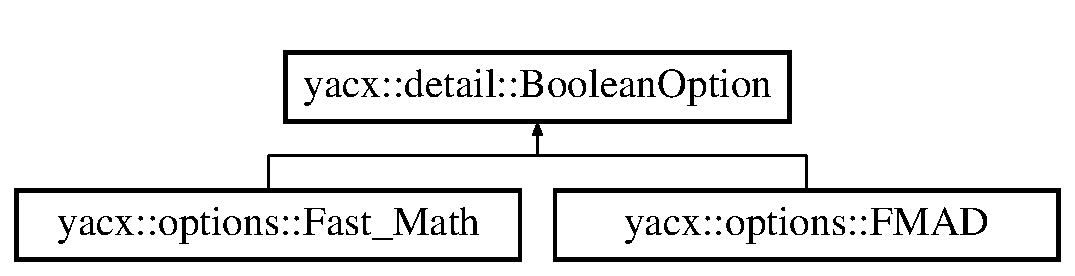
\includegraphics[height=2.000000cm]{classyacx_1_1detail_1_1_boolean_option}
\end{center}
\end{figure}
\subsection*{Public Member Functions}
\begin{DoxyCompactItemize}
\item 
\mbox{\Hypertarget{classyacx_1_1detail_1_1_boolean_option_a4805b9e0ac55b8b3d24531e8dd768790}\label{classyacx_1_1detail_1_1_boolean_option_a4805b9e0ac55b8b3d24531e8dd768790}} 
{\bfseries Boolean\+Option} (bool b)
\item 
\mbox{\Hypertarget{classyacx_1_1detail_1_1_boolean_option_aaa668d25a0bf023ec7f6bc0387836c43}\label{classyacx_1_1detail_1_1_boolean_option_aaa668d25a0bf023ec7f6bc0387836c43}} 
auto {\bfseries value} () const
\end{DoxyCompactItemize}


The documentation for this class was generated from the following file\+:\begin{DoxyCompactItemize}
\item 
include/yacx/Options.\+hpp\end{DoxyCompactItemize}

\hypertarget{classyacx_1_1_c_program}{}\doxysection{yacx\+::C\+Program Class Reference}
\label{classyacx_1_1_c_program}\index{yacx::CProgram@{yacx::CProgram}}
Inheritance diagram for yacx\+::C\+Program\+:\begin{figure}[H]
\begin{center}
\leavevmode
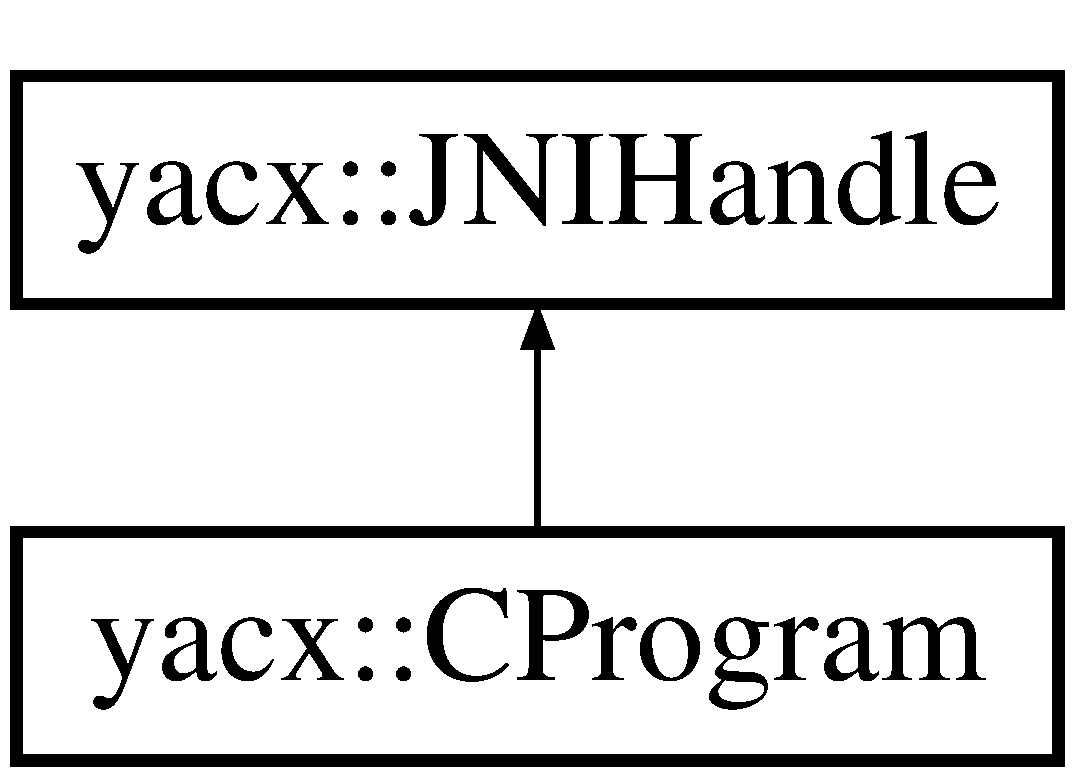
\includegraphics[height=2.000000cm]{classyacx_1_1_c_program}
\end{center}
\end{figure}
\doxysubsection*{Public Member Functions}
\begin{DoxyCompactItemize}
\item 
\mbox{\hyperlink{classyacx_1_1_c_program_aa5c8ed40dc90db7652fd0b0924297a45}{C\+Program}} (const char $\ast$c\+Program, const char $\ast$function\+Name, std\+::vector$<$ std\+::string $>$ \&parameter\+Types, const char $\ast$compiler=\char`\"{}gcc\char`\"{}, Options \&options=D\+E\+F\+A\+U\+L\+T\+\_\+\+O\+P\+T\+I\+O\+NS)
\item 
void \mbox{\hyperlink{classyacx_1_1_c_program_a50cc4f5ca3826b1e3dd870e1d5e17e89}{execute}} (std\+::vector$<$ void $\ast$ $>$ arguments)
\end{DoxyCompactItemize}


\doxysubsection{Constructor \& Destructor Documentation}
\mbox{\Hypertarget{classyacx_1_1_c_program_aa5c8ed40dc90db7652fd0b0924297a45}\label{classyacx_1_1_c_program_aa5c8ed40dc90db7652fd0b0924297a45}} 
\index{yacx::CProgram@{yacx::CProgram}!CProgram@{CProgram}}
\index{CProgram@{CProgram}!yacx::CProgram@{yacx::CProgram}}
\doxysubsubsection{\texorpdfstring{CProgram()}{CProgram()}}
{\footnotesize\ttfamily C\+Program\+::\+C\+Program (\begin{DoxyParamCaption}\item[{const char $\ast$}]{c\+Program,  }\item[{const char $\ast$}]{function\+Name,  }\item[{std\+::vector$<$ std\+::string $>$ \&}]{parameter\+Types,  }\item[{const char $\ast$}]{compiler = {\ttfamily \char`\"{}gcc\char`\"{}},  }\item[{\mbox{\hyperlink{classyacx_1_1_options}{Options}} \&}]{options = {\ttfamily DEFAULT\+\_\+OPTIONS} }\end{DoxyParamCaption})}

Constructs new compiled \mbox{\hyperlink{classyacx_1_1_c_program}{C\+Program}}. ~\newline
 The decleration of structs, functions or variables with one of the following name within passed C-\/\+Code is permitted\+: ~\newline
 op$<$function\+Name$>$, opfn$<$function\+Name$>$, execute$<$function\+Name$>$
\begin{DoxyParams}{Parameters}
{\em c\+Program} & C-\/\+Code for program\\
\hline
{\em function\+Name} & name of c-\/function, which should be executed \\
\hline
{\em parameter\+Types} & type of the parameters e.\+g {\ttfamily int} or {\ttfamily float$\ast$} ~\newline
 pointer types can be abbreviated by $\ast$\\
\hline
{\em compiler} & name of the compiler, which should be used to compile this c\+Program\\
\hline
{\em options} & options for the compiler \\
\hline
\end{DoxyParams}


\doxysubsection{Member Function Documentation}
\mbox{\Hypertarget{classyacx_1_1_c_program_a50cc4f5ca3826b1e3dd870e1d5e17e89}\label{classyacx_1_1_c_program_a50cc4f5ca3826b1e3dd870e1d5e17e89}} 
\index{yacx::CProgram@{yacx::CProgram}!execute@{execute}}
\index{execute@{execute}!yacx::CProgram@{yacx::CProgram}}
\doxysubsubsection{\texorpdfstring{execute()}{execute()}}
{\footnotesize\ttfamily void C\+Program\+::execute (\begin{DoxyParamCaption}\item[{std\+::vector$<$ void $\ast$ $>$}]{arguments }\end{DoxyParamCaption})}

Executes a the c\+Function 
\begin{DoxyParams}{Parameters}
{\em arguments} & arguments for the c\+Function \\
\hline
\end{DoxyParams}


The documentation for this class was generated from the following files\+:\begin{DoxyCompactItemize}
\item 
include/yacx/cexecutor/C\+Program.\+hpp\item 
src/cexecutor/C\+Program.\+cpp\end{DoxyCompactItemize}

\hypertarget{classyacx_1_1_c_uresult_exception}{}\doxysection{yacx\+::C\+Uresult\+Exception Class Reference}
\label{classyacx_1_1_c_uresult_exception}\index{yacx::CUresultException@{yacx::CUresultException}}


Exception class for C\+U\+DA driver api errors.  




{\ttfamily \#include $<$Exception.\+hpp$>$}

Inheritance diagram for yacx\+::C\+Uresult\+Exception\+:\begin{figure}[H]
\begin{center}
\leavevmode
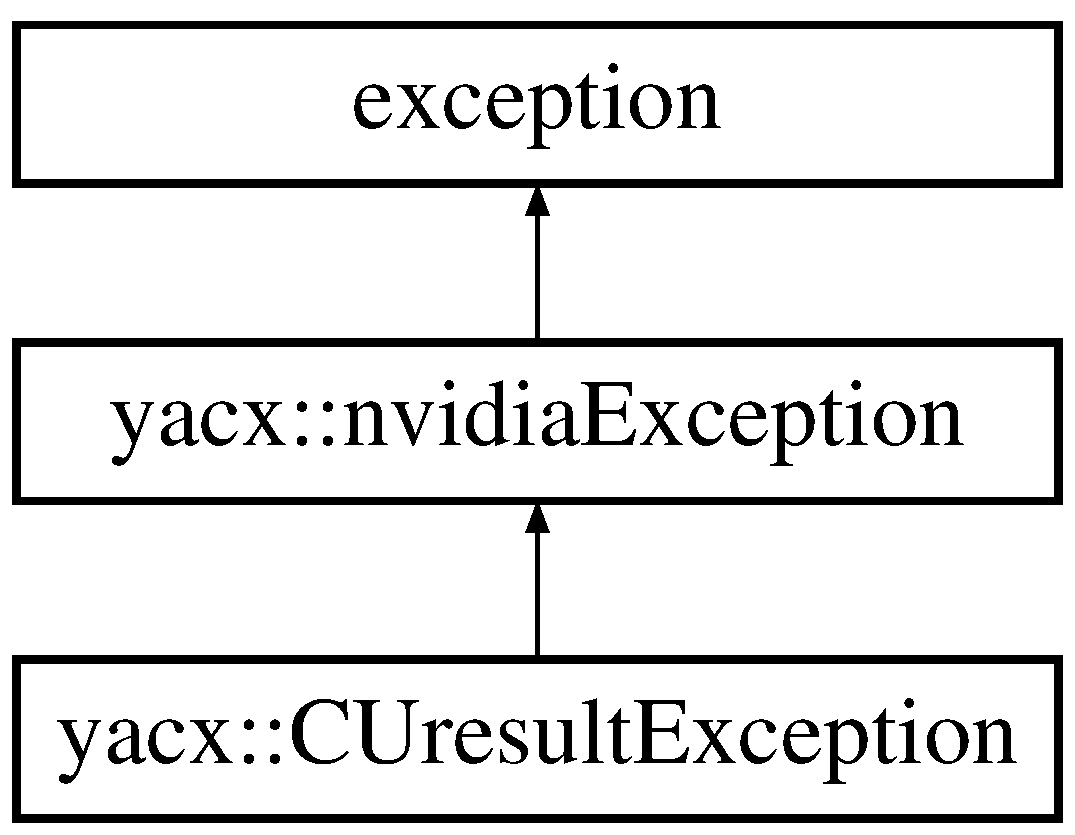
\includegraphics[height=3.000000cm]{classyacx_1_1_c_uresult_exception}
\end{center}
\end{figure}
\doxysubsection*{Public Member Functions}
\begin{DoxyCompactItemize}
\item 
\mbox{\Hypertarget{classyacx_1_1_c_uresult_exception_a8b3eabebd5354aa149ee6e2b1fe8f67e}\label{classyacx_1_1_c_uresult_exception_a8b3eabebd5354aa149ee6e2b1fe8f67e}} 
{\bfseries C\+Uresult\+Exception} (C\+Uresult type, std\+::string error)
\end{DoxyCompactItemize}
\doxysubsection*{Public Attributes}
\begin{DoxyCompactItemize}
\item 
\mbox{\Hypertarget{classyacx_1_1_c_uresult_exception_a1b3e9c65d733f43ff37a69b432e73216}\label{classyacx_1_1_c_uresult_exception_a1b3e9c65d733f43ff37a69b432e73216}} 
C\+Uresult {\bfseries type}
\end{DoxyCompactItemize}
\doxysubsection*{Additional Inherited Members}


\doxysubsection{Detailed Description}
Exception class for C\+U\+DA driver api errors. 


\begin{DoxyTemplParams}{Template Parameters}
{\em type} & Name and type of the C\+U\+DA Error, e.\+g. {\ttfamily C\+U\+D\+A\+\_\+\+E\+R\+R\+O\+R\+\_\+\+N\+O\+\_\+\+D\+E\+V\+I\+CE} \\
\hline
{\em error} & descripton of error \\
\hline
\end{DoxyTemplParams}
\begin{Desc}
\item[Examples]\par
\mbox{\hyperlink{docs_2cudaexeption_8cpp-example}{docs/cudaexeption.\+cpp}}.\end{Desc}


The documentation for this class was generated from the following file\+:\begin{DoxyCompactItemize}
\item 
include/yacx/Exception.\+hpp\end{DoxyCompactItemize}

\hypertarget{classyacx_1_1detail_1_1_data_copy}{}\doxysection{yacx\+::detail\+::Data\+Copy Class Reference}
\label{classyacx_1_1detail_1_1_data_copy}\index{yacx::detail::DataCopy@{yacx::detail::DataCopy}}
Inheritance diagram for yacx\+::detail\+::Data\+Copy\+:\begin{figure}[H]
\begin{center}
\leavevmode
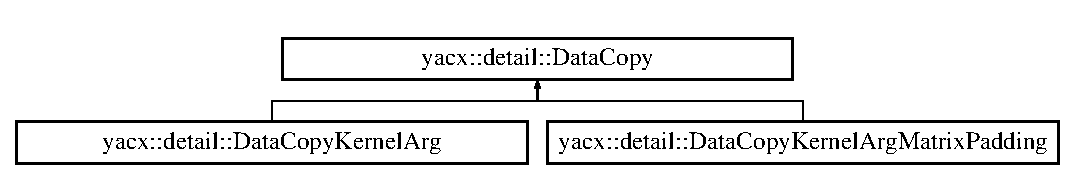
\includegraphics[height=1.971831cm]{classyacx_1_1detail_1_1_data_copy}
\end{center}
\end{figure}
\doxysubsection*{Public Member Functions}
\begin{DoxyCompactItemize}
\item 
\mbox{\Hypertarget{classyacx_1_1detail_1_1_data_copy_aec6fe17c8a22b1ad61cb2f1a45f96591}\label{classyacx_1_1detail_1_1_data_copy_aec6fe17c8a22b1ad61cb2f1a45f96591}} 
\mbox{\hyperlink{classyacx_1_1detail_1_1_data_copy_aec6fe17c8a22b1ad61cb2f1a45f96591}{Data\+Copy}} ()
\begin{DoxyCompactList}\small\item\em A constructor. \end{DoxyCompactList}\item 
virtual void \mbox{\hyperlink{classyacx_1_1detail_1_1_data_copy_ad528786c51783257b292a06a6dde1c4e}{copy\+Data\+HtoD}} (void $\ast$hdata, C\+Udeviceptr ddata, size\+\_\+t size, C\+Ustream stream)=0
\item 
virtual void \mbox{\hyperlink{classyacx_1_1detail_1_1_data_copy_ab97df2d6bec15f8247a5da0ff8bd05ff}{copy\+Data\+DtoH}} (C\+Udeviceptr ddata, void $\ast$hdata, size\+\_\+t size, C\+Ustream stream)=0
\end{DoxyCompactItemize}


\doxysubsection{Member Function Documentation}
\mbox{\Hypertarget{classyacx_1_1detail_1_1_data_copy_ab97df2d6bec15f8247a5da0ff8bd05ff}\label{classyacx_1_1detail_1_1_data_copy_ab97df2d6bec15f8247a5da0ff8bd05ff}} 
\index{yacx::detail::DataCopy@{yacx::detail::DataCopy}!copyDataDtoH@{copyDataDtoH}}
\index{copyDataDtoH@{copyDataDtoH}!yacx::detail::DataCopy@{yacx::detail::DataCopy}}
\doxysubsubsection{\texorpdfstring{copyDataDtoH()}{copyDataDtoH()}}
{\footnotesize\ttfamily virtual void yacx\+::detail\+::\+Data\+Copy\+::copy\+Data\+DtoH (\begin{DoxyParamCaption}\item[{C\+Udeviceptr}]{ddata,  }\item[{void $\ast$}]{hdata,  }\item[{size\+\_\+t}]{size,  }\item[{C\+Ustream}]{stream }\end{DoxyParamCaption})\hspace{0.3cm}{\ttfamily [pure virtual]}}

copy data from device to host 
\begin{DoxyParams}{Parameters}
{\em ddata} & pointer to device data \\
\hline
{\em hdata} & pointer to host data \\
\hline
{\em size} & size of the data \\
\hline
\end{DoxyParams}


Implemented in \mbox{\hyperlink{classyacx_1_1detail_1_1_data_copy_kernel_arg_matrix_padding_ac76365a728b5cd0f7e2bd65051b4912e}{yacx\+::detail\+::\+Data\+Copy\+Kernel\+Arg\+Matrix\+Padding}}, and \mbox{\hyperlink{classyacx_1_1detail_1_1_data_copy_kernel_arg_a1a6b70eea2dde6b360a1af77414dfa9f}{yacx\+::detail\+::\+Data\+Copy\+Kernel\+Arg}}.

\mbox{\Hypertarget{classyacx_1_1detail_1_1_data_copy_ad528786c51783257b292a06a6dde1c4e}\label{classyacx_1_1detail_1_1_data_copy_ad528786c51783257b292a06a6dde1c4e}} 
\index{yacx::detail::DataCopy@{yacx::detail::DataCopy}!copyDataHtoD@{copyDataHtoD}}
\index{copyDataHtoD@{copyDataHtoD}!yacx::detail::DataCopy@{yacx::detail::DataCopy}}
\doxysubsubsection{\texorpdfstring{copyDataHtoD()}{copyDataHtoD()}}
{\footnotesize\ttfamily virtual void yacx\+::detail\+::\+Data\+Copy\+::copy\+Data\+HtoD (\begin{DoxyParamCaption}\item[{void $\ast$}]{hdata,  }\item[{C\+Udeviceptr}]{ddata,  }\item[{size\+\_\+t}]{size,  }\item[{C\+Ustream}]{stream }\end{DoxyParamCaption})\hspace{0.3cm}{\ttfamily [pure virtual]}}

copy data from host to device 
\begin{DoxyParams}{Parameters}
{\em hdata} & pointer to host data \\
\hline
{\em ddata} & pointer to device data \\
\hline
{\em size} & size of the data \\
\hline
\end{DoxyParams}


Implemented in \mbox{\hyperlink{classyacx_1_1detail_1_1_data_copy_kernel_arg_matrix_padding_a61ebfbf622e637145db249302c230873}{yacx\+::detail\+::\+Data\+Copy\+Kernel\+Arg\+Matrix\+Padding}}, and \mbox{\hyperlink{classyacx_1_1detail_1_1_data_copy_kernel_arg_a0cf2b2af95ca2c01b1a221a14a95e558}{yacx\+::detail\+::\+Data\+Copy\+Kernel\+Arg}}.



The documentation for this class was generated from the following file\+:\begin{DoxyCompactItemize}
\item 
include/yacx/Kernel\+Args.\+hpp\end{DoxyCompactItemize}

\hypertarget{classyacx_1_1detail_1_1_data_copy_kernel_arg}{}\section{yacx\+:\+:detail\+:\+:Data\+Copy\+Kernel\+Arg Class Reference}
\label{classyacx_1_1detail_1_1_data_copy_kernel_arg}\index{yacx\+::detail\+::\+Data\+Copy\+Kernel\+Arg@{yacx\+::detail\+::\+Data\+Copy\+Kernel\+Arg}}
Inheritance diagram for yacx\+:\+:detail\+:\+:Data\+Copy\+Kernel\+Arg\+:\begin{figure}[H]
\begin{center}
\leavevmode
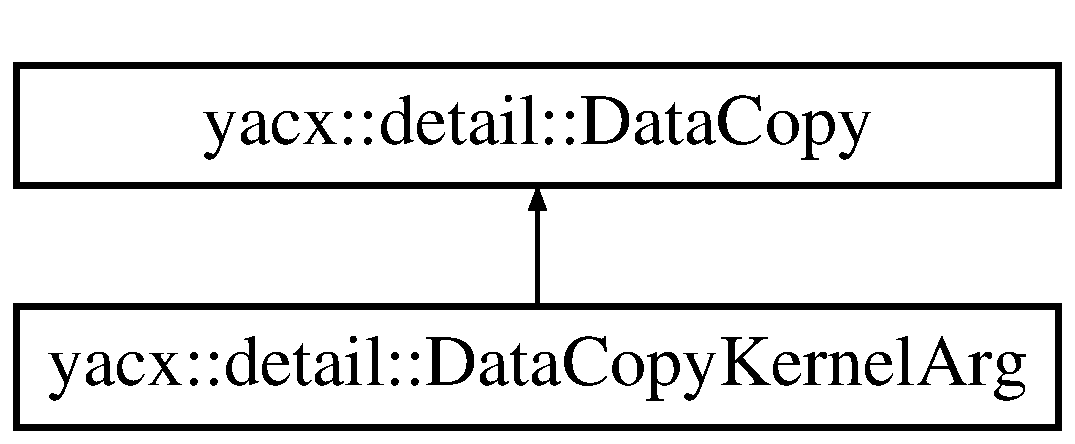
\includegraphics[height=2.000000cm]{classyacx_1_1detail_1_1_data_copy_kernel_arg}
\end{center}
\end{figure}
\subsection*{Public Member Functions}
\begin{DoxyCompactItemize}
\item 
void \hyperlink{classyacx_1_1detail_1_1_data_copy_kernel_arg_a0cf2b2af95ca2c01b1a221a14a95e558}{copy\+Data\+HtoD} (void $\ast$hdata, C\+Udeviceptr ddata, size\+\_\+t size, C\+Ustream stream) override
\item 
void \hyperlink{classyacx_1_1detail_1_1_data_copy_kernel_arg_a1a6b70eea2dde6b360a1af77414dfa9f}{copy\+Data\+DtoH} (C\+Udeviceptr ddata, void $\ast$hdata, size\+\_\+t size, C\+Ustream stream) override
\end{DoxyCompactItemize}


\subsection{Member Function Documentation}
\mbox{\Hypertarget{classyacx_1_1detail_1_1_data_copy_kernel_arg_a1a6b70eea2dde6b360a1af77414dfa9f}\label{classyacx_1_1detail_1_1_data_copy_kernel_arg_a1a6b70eea2dde6b360a1af77414dfa9f}} 
\index{yacx\+::detail\+::\+Data\+Copy\+Kernel\+Arg@{yacx\+::detail\+::\+Data\+Copy\+Kernel\+Arg}!copy\+Data\+DtoH@{copy\+Data\+DtoH}}
\index{copy\+Data\+DtoH@{copy\+Data\+DtoH}!yacx\+::detail\+::\+Data\+Copy\+Kernel\+Arg@{yacx\+::detail\+::\+Data\+Copy\+Kernel\+Arg}}
\subsubsection{\texorpdfstring{copy\+Data\+Dto\+H()}{copyDataDtoH()}}
{\footnotesize\ttfamily void Data\+Copy\+Kernel\+Arg\+::copy\+Data\+DtoH (\begin{DoxyParamCaption}\item[{C\+Udeviceptr}]{ddata,  }\item[{void $\ast$}]{hdata,  }\item[{size\+\_\+t}]{size,  }\item[{C\+Ustream}]{stream }\end{DoxyParamCaption})\hspace{0.3cm}{\ttfamily [override]}, {\ttfamily [virtual]}}

copy data from device to host 
\begin{DoxyParams}{Parameters}
{\em ddata} & pointer to device data \\
\hline
{\em hdata} & pointer to host data \\
\hline
{\em size} & size of the data \\
\hline
\end{DoxyParams}


Implements \hyperlink{classyacx_1_1detail_1_1_data_copy_ab97df2d6bec15f8247a5da0ff8bd05ff}{yacx\+::detail\+::\+Data\+Copy}.

\mbox{\Hypertarget{classyacx_1_1detail_1_1_data_copy_kernel_arg_a0cf2b2af95ca2c01b1a221a14a95e558}\label{classyacx_1_1detail_1_1_data_copy_kernel_arg_a0cf2b2af95ca2c01b1a221a14a95e558}} 
\index{yacx\+::detail\+::\+Data\+Copy\+Kernel\+Arg@{yacx\+::detail\+::\+Data\+Copy\+Kernel\+Arg}!copy\+Data\+HtoD@{copy\+Data\+HtoD}}
\index{copy\+Data\+HtoD@{copy\+Data\+HtoD}!yacx\+::detail\+::\+Data\+Copy\+Kernel\+Arg@{yacx\+::detail\+::\+Data\+Copy\+Kernel\+Arg}}
\subsubsection{\texorpdfstring{copy\+Data\+Hto\+D()}{copyDataHtoD()}}
{\footnotesize\ttfamily void Data\+Copy\+Kernel\+Arg\+::copy\+Data\+HtoD (\begin{DoxyParamCaption}\item[{void $\ast$}]{hdata,  }\item[{C\+Udeviceptr}]{ddata,  }\item[{size\+\_\+t}]{size,  }\item[{C\+Ustream}]{stream }\end{DoxyParamCaption})\hspace{0.3cm}{\ttfamily [override]}, {\ttfamily [virtual]}}

copy data from host to device 
\begin{DoxyParams}{Parameters}
{\em hdata} & pointer to host data \\
\hline
{\em ddata} & pointer to device data \\
\hline
{\em size} & size of the data \\
\hline
\end{DoxyParams}


Implements \hyperlink{classyacx_1_1detail_1_1_data_copy_ad528786c51783257b292a06a6dde1c4e}{yacx\+::detail\+::\+Data\+Copy}.



The documentation for this class was generated from the following files\+:\begin{DoxyCompactItemize}
\item 
include/yacx/Kernel\+Args.\+hpp\item 
src/Kernel\+Arg.\+cpp\end{DoxyCompactItemize}

\hypertarget{classyacx_1_1detail_1_1_data_copy_kernel_arg_matrix_padding}{}\section{yacx\+:\+:detail\+:\+:Data\+Copy\+Kernel\+Arg\+Matrix\+Padding Class Reference}
\label{classyacx_1_1detail_1_1_data_copy_kernel_arg_matrix_padding}\index{yacx\+::detail\+::\+Data\+Copy\+Kernel\+Arg\+Matrix\+Padding@{yacx\+::detail\+::\+Data\+Copy\+Kernel\+Arg\+Matrix\+Padding}}
Inheritance diagram for yacx\+:\+:detail\+:\+:Data\+Copy\+Kernel\+Arg\+Matrix\+Padding\+:\begin{figure}[H]
\begin{center}
\leavevmode
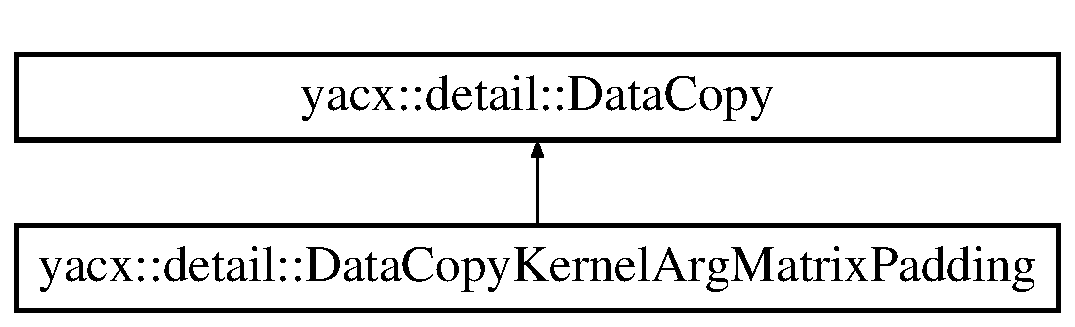
\includegraphics[height=2.000000cm]{classyacx_1_1detail_1_1_data_copy_kernel_arg_matrix_padding}
\end{center}
\end{figure}
\subsection*{Public Member Functions}
\begin{DoxyCompactItemize}
\item 
\hyperlink{classyacx_1_1detail_1_1_data_copy_kernel_arg_matrix_padding_a77b442a566bffe4b5ceac055de047241}{Data\+Copy\+Kernel\+Arg\+Matrix\+Padding} (int element\+Size, unsigned int padding\+Value, int src\+\_\+rows, int src\+\_\+columns, int dst\+\_\+rows, int dst\+\_\+columns)
\begin{DoxyCompactList}\small\item\em A constructor. \end{DoxyCompactList}\item 
void \hyperlink{classyacx_1_1detail_1_1_data_copy_kernel_arg_matrix_padding_a61ebfbf622e637145db249302c230873}{copy\+Data\+HtoD} (void $\ast$hdata, C\+Udeviceptr ddata, size\+\_\+t size, C\+Ustream stream) override
\item 
void \hyperlink{classyacx_1_1detail_1_1_data_copy_kernel_arg_matrix_padding_ac76365a728b5cd0f7e2bd65051b4912e}{copy\+Data\+DtoH} (C\+Udeviceptr ddata, void $\ast$hdata, size\+\_\+t size, C\+Ustream stream) override
\end{DoxyCompactItemize}


\subsection{Constructor \& Destructor Documentation}
\mbox{\Hypertarget{classyacx_1_1detail_1_1_data_copy_kernel_arg_matrix_padding_a77b442a566bffe4b5ceac055de047241}\label{classyacx_1_1detail_1_1_data_copy_kernel_arg_matrix_padding_a77b442a566bffe4b5ceac055de047241}} 
\index{yacx\+::detail\+::\+Data\+Copy\+Kernel\+Arg\+Matrix\+Padding@{yacx\+::detail\+::\+Data\+Copy\+Kernel\+Arg\+Matrix\+Padding}!Data\+Copy\+Kernel\+Arg\+Matrix\+Padding@{Data\+Copy\+Kernel\+Arg\+Matrix\+Padding}}
\index{Data\+Copy\+Kernel\+Arg\+Matrix\+Padding@{Data\+Copy\+Kernel\+Arg\+Matrix\+Padding}!yacx\+::detail\+::\+Data\+Copy\+Kernel\+Arg\+Matrix\+Padding@{yacx\+::detail\+::\+Data\+Copy\+Kernel\+Arg\+Matrix\+Padding}}
\subsubsection{\texorpdfstring{Data\+Copy\+Kernel\+Arg\+Matrix\+Padding()}{DataCopyKernelArgMatrixPadding()}}
{\footnotesize\ttfamily yacx\+::detail\+::\+Data\+Copy\+Kernel\+Arg\+Matrix\+Padding\+::\+Data\+Copy\+Kernel\+Arg\+Matrix\+Padding (\begin{DoxyParamCaption}\item[{int}]{element\+Size,  }\item[{unsigned int}]{padding\+Value,  }\item[{int}]{src\+\_\+rows,  }\item[{int}]{src\+\_\+columns,  }\item[{int}]{dst\+\_\+rows,  }\item[{int}]{dst\+\_\+columns }\end{DoxyParamCaption})\hspace{0.3cm}{\ttfamily [inline]}}



A constructor. 


\begin{DoxyParams}{Parameters}
{\em element\+Size} & size of each element of the matrix in bytes \\
\hline
{\em padding\+Value} & value to fill up additional rows and columns \\
\hline
{\em src\+\_\+rows} & number of rows of current matrix without padding \\
\hline
{\em src\+\_\+columns} & number of columns of currentmatrix without padding \\
\hline
{\em dst\+\_\+rows} & number of rows for new matrix with padding \\
\hline
{\em dst\+\_\+columns} & number of columns for new matrix with padding \\
\hline
\end{DoxyParams}


\subsection{Member Function Documentation}
\mbox{\Hypertarget{classyacx_1_1detail_1_1_data_copy_kernel_arg_matrix_padding_ac76365a728b5cd0f7e2bd65051b4912e}\label{classyacx_1_1detail_1_1_data_copy_kernel_arg_matrix_padding_ac76365a728b5cd0f7e2bd65051b4912e}} 
\index{yacx\+::detail\+::\+Data\+Copy\+Kernel\+Arg\+Matrix\+Padding@{yacx\+::detail\+::\+Data\+Copy\+Kernel\+Arg\+Matrix\+Padding}!copy\+Data\+DtoH@{copy\+Data\+DtoH}}
\index{copy\+Data\+DtoH@{copy\+Data\+DtoH}!yacx\+::detail\+::\+Data\+Copy\+Kernel\+Arg\+Matrix\+Padding@{yacx\+::detail\+::\+Data\+Copy\+Kernel\+Arg\+Matrix\+Padding}}
\subsubsection{\texorpdfstring{copy\+Data\+Dto\+H()}{copyDataDtoH()}}
{\footnotesize\ttfamily void Data\+Copy\+Kernel\+Arg\+Matrix\+Padding\+::copy\+Data\+DtoH (\begin{DoxyParamCaption}\item[{C\+Udeviceptr}]{ddata,  }\item[{void $\ast$}]{hdata,  }\item[{size\+\_\+t}]{size,  }\item[{C\+Ustream}]{stream }\end{DoxyParamCaption})\hspace{0.3cm}{\ttfamily [override]}, {\ttfamily [virtual]}}

copy data from device to host 
\begin{DoxyParams}{Parameters}
{\em ddata} & pointer to device data \\
\hline
{\em hdata} & pointer to host data \\
\hline
{\em size} & size of the data \\
\hline
\end{DoxyParams}


Implements \hyperlink{classyacx_1_1detail_1_1_data_copy_ab97df2d6bec15f8247a5da0ff8bd05ff}{yacx\+::detail\+::\+Data\+Copy}.

\mbox{\Hypertarget{classyacx_1_1detail_1_1_data_copy_kernel_arg_matrix_padding_a61ebfbf622e637145db249302c230873}\label{classyacx_1_1detail_1_1_data_copy_kernel_arg_matrix_padding_a61ebfbf622e637145db249302c230873}} 
\index{yacx\+::detail\+::\+Data\+Copy\+Kernel\+Arg\+Matrix\+Padding@{yacx\+::detail\+::\+Data\+Copy\+Kernel\+Arg\+Matrix\+Padding}!copy\+Data\+HtoD@{copy\+Data\+HtoD}}
\index{copy\+Data\+HtoD@{copy\+Data\+HtoD}!yacx\+::detail\+::\+Data\+Copy\+Kernel\+Arg\+Matrix\+Padding@{yacx\+::detail\+::\+Data\+Copy\+Kernel\+Arg\+Matrix\+Padding}}
\subsubsection{\texorpdfstring{copy\+Data\+Hto\+D()}{copyDataHtoD()}}
{\footnotesize\ttfamily void Data\+Copy\+Kernel\+Arg\+Matrix\+Padding\+::copy\+Data\+HtoD (\begin{DoxyParamCaption}\item[{void $\ast$}]{hdata,  }\item[{C\+Udeviceptr}]{ddata,  }\item[{size\+\_\+t}]{size,  }\item[{C\+Ustream}]{stream }\end{DoxyParamCaption})\hspace{0.3cm}{\ttfamily [override]}, {\ttfamily [virtual]}}

copy data from host to device 
\begin{DoxyParams}{Parameters}
{\em hdata} & pointer to host data \\
\hline
{\em ddata} & pointer to device data \\
\hline
{\em size} & size of the data \\
\hline
\end{DoxyParams}


Implements \hyperlink{classyacx_1_1detail_1_1_data_copy_ad528786c51783257b292a06a6dde1c4e}{yacx\+::detail\+::\+Data\+Copy}.



The documentation for this class was generated from the following files\+:\begin{DoxyCompactItemize}
\item 
include/yacx/Kernel\+Args.\+hpp\item 
src/Kernel\+Arg.\+cpp\end{DoxyCompactItemize}

\hypertarget{classyacx_1_1_device}{}\doxysection{yacx\+::Device Class Reference}
\label{classyacx_1_1_device}\index{yacx::Device@{yacx::Device}}
Inheritance diagram for yacx\+::Device\+:\begin{figure}[H]
\begin{center}
\leavevmode
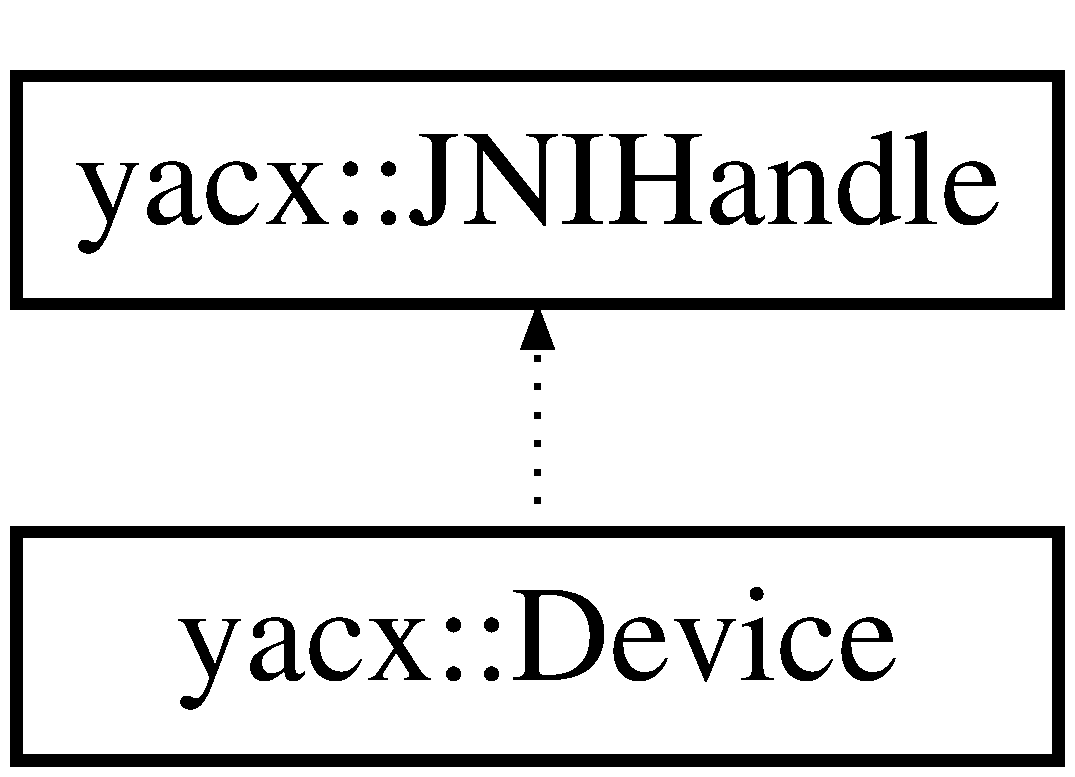
\includegraphics[height=2.000000cm]{classyacx_1_1_device}
\end{center}
\end{figure}
\doxysubsection*{Public Member Functions}
\begin{DoxyCompactItemize}
\item 
\mbox{\Hypertarget{classyacx_1_1_device_a4d6a77e872d111010c7f7e246cb412a4}\label{classyacx_1_1_device_a4d6a77e872d111010c7f7e246cb412a4}} 
\mbox{\hyperlink{classyacx_1_1_device_a4d6a77e872d111010c7f7e246cb412a4}{Device}} (int ordinal)
\begin{DoxyCompactList}\small\item\em Constructs a \mbox{\hyperlink{classyacx_1_1_device}{Device}} with the C\+U\+DA capable device with passed devicenumber. \end{DoxyCompactList}\item 
\mbox{\Hypertarget{classyacx_1_1_device_ab661f7dcdc107c892064cc7c52e2b0f9}\label{classyacx_1_1_device_ab661f7dcdc107c892064cc7c52e2b0f9}} 
\mbox{\hyperlink{classyacx_1_1_device_ab661f7dcdc107c892064cc7c52e2b0f9}{Device}} ()
\begin{DoxyCompactList}\small\item\em Constructs a \mbox{\hyperlink{classyacx_1_1_device}{Device}} with the first C\+U\+DA capable device it finds. \end{DoxyCompactList}\item 
int \mbox{\hyperlink{classyacx_1_1_device_a5d7a0d5f9c543768323cfc8807d9aa27}{minor\+\_\+version}} () const
\item 
int \mbox{\hyperlink{classyacx_1_1_device_ac72d60151e4070d118cd0aadd0d7d448}{major\+\_\+version}} () const
\item 
std\+::string \mbox{\hyperlink{classyacx_1_1_device_a49388d8375dc98070973470f6cd997e8}{name}} () const
\item 
C\+Ucontext \mbox{\hyperlink{classyacx_1_1_device_a9227417e61e545bed24aeb72272bf277}{get\+Primary\+Context}} ()
\item 
C\+Ustream \mbox{\hyperlink{classyacx_1_1_device_a9b226ea765e496ca388a466875f40d72}{get\+Upload\+Stream}} ()
\item 
C\+Ustream \mbox{\hyperlink{classyacx_1_1_device_a51d568a0c576533dab7a3d2bbe5c2214}{get\+Launch\+Stream}} ()
\item 
C\+Ustream \mbox{\hyperlink{classyacx_1_1_device_a5304b1ba9e1fc512caa64041b39f13fd}{get\+Download\+Stream}} ()
\item 
size\+\_\+t \mbox{\hyperlink{classyacx_1_1_device_a14acbcda1fdf398b018ee329406b9c7b}{total\+\_\+memory}} () const
\item 
std\+::string \mbox{\hyperlink{classyacx_1_1_device_a1fcf245197f59b939e36c24771ee07d3}{uuid}} () const
\item 
dim3 \mbox{\hyperlink{classyacx_1_1_device_a34e5cca7423047044ac3e683bf0eb2f9}{max\+\_\+block\+\_\+dim}} ()
\item 
dim3 \mbox{\hyperlink{classyacx_1_1_device_a28355cb20ff6755dd958082540013600}{max\+\_\+grid\+\_\+dim}} ()
\item 
size\+\_\+t \mbox{\hyperlink{classyacx_1_1_device_a76378cc2e3f33e4c714296843236be4b}{max\+\_\+shared\+\_\+memory\+\_\+per\+\_\+block}} () const
\item 
size\+\_\+t \mbox{\hyperlink{classyacx_1_1_device_ac1dcf4a775430a5334eb5c51586a69a2}{max\+\_\+shared\+\_\+memory\+\_\+per\+\_\+multiprocessor}} () const
\item 
size\+\_\+t \mbox{\hyperlink{classyacx_1_1_device_ae97aae54e13c2be6acbb1d0992ddd473}{multiprocessor\+\_\+count}} () const
\item 
int \mbox{\hyperlink{classyacx_1_1_device_a74c7ad2bea44bf536f35c79b9f19528a}{clock\+\_\+rate}} () const
\item 
int \mbox{\hyperlink{classyacx_1_1_device_a41a46878ca07cfbbfd553aeae6076e63}{memory\+\_\+clock\+\_\+rate}} () const
\item 
int \mbox{\hyperlink{classyacx_1_1_device_aaec2c2024842d546c46e7ab45abce8c5}{bus\+\_\+width}} () const
\item 
int \mbox{\hyperlink{classyacx_1_1_device_aff8748b38646df669d7b29d03dc18077}{attribute}} (C\+Udevice\+\_\+attribute attrib) const
\end{DoxyCompactItemize}
\doxysubsection*{Friends}
\begin{DoxyCompactItemize}
\item 
\mbox{\Hypertarget{classyacx_1_1_device_a26656a71544c176b6a5f20be8773de3f}\label{classyacx_1_1_device_a26656a71544c176b6a5f20be8773de3f}} 
class {\bfseries Devices}
\end{DoxyCompactItemize}


\doxysubsection{Detailed Description}
\begin{Desc}
\item[Examples]\par
\mbox{\hyperlink{docs_2kernel_launch_8cpp-example}{docs/kernel\+\_\+launch.\+cpp}}, \mbox{\hyperlink{example_matrix_multiply_8cpp-example}{example\+\_\+matrix\+\_\+multiply.\+cpp}}, \mbox{\hyperlink{example_program_8cpp-example}{example\+\_\+program.\+cpp}}, and \mbox{\hyperlink{example_saxpy_8cpp-example}{example\+\_\+saxpy.\+cpp}}.\end{Desc}


\doxysubsection{Member Function Documentation}
\mbox{\Hypertarget{classyacx_1_1_device_aff8748b38646df669d7b29d03dc18077}\label{classyacx_1_1_device_aff8748b38646df669d7b29d03dc18077}} 
\index{yacx::Device@{yacx::Device}!attribute@{attribute}}
\index{attribute@{attribute}!yacx::Device@{yacx::Device}}
\doxysubsubsection{\texorpdfstring{attribute()}{attribute()}}
{\footnotesize\ttfamily int Device\+::attribute (\begin{DoxyParamCaption}\item[{C\+Udevice\+\_\+attribute}]{attrib }\end{DoxyParamCaption}) const}

Returns information about the device, see \href{https://docs.nvidia.com/cuda/cuda-driver-api/group__CUDA__DEVICE.html\#group__CUDA__DEVICE_1g9c3e1414f0ad901d3278a4d6645fc266}{\texttt{ C\+Udevice\+\_\+attribute}} 
\begin{DoxyParams}{Parameters}
{\em attrib} & C\+U\+DA device attribute \\
\hline
\end{DoxyParams}
\begin{DoxyReturn}{Returns}
device attribute value 
\end{DoxyReturn}
\mbox{\Hypertarget{classyacx_1_1_device_aaec2c2024842d546c46e7ab45abce8c5}\label{classyacx_1_1_device_aaec2c2024842d546c46e7ab45abce8c5}} 
\index{yacx::Device@{yacx::Device}!bus\_width@{bus\_width}}
\index{bus\_width@{bus\_width}!yacx::Device@{yacx::Device}}
\doxysubsubsection{\texorpdfstring{bus\_width()}{bus\_width()}}
{\footnotesize\ttfamily int yacx\+::\+Device\+::bus\+\_\+width (\begin{DoxyParamCaption}{ }\end{DoxyParamCaption}) const\hspace{0.3cm}{\ttfamily [inline]}}

Global memory bus width in bits \begin{DoxyReturn}{Returns}
bus width 
\end{DoxyReturn}
\mbox{\Hypertarget{classyacx_1_1_device_a74c7ad2bea44bf536f35c79b9f19528a}\label{classyacx_1_1_device_a74c7ad2bea44bf536f35c79b9f19528a}} 
\index{yacx::Device@{yacx::Device}!clock\_rate@{clock\_rate}}
\index{clock\_rate@{clock\_rate}!yacx::Device@{yacx::Device}}
\doxysubsubsection{\texorpdfstring{clock\_rate()}{clock\_rate()}}
{\footnotesize\ttfamily int yacx\+::\+Device\+::clock\+\_\+rate (\begin{DoxyParamCaption}{ }\end{DoxyParamCaption}) const\hspace{0.3cm}{\ttfamily [inline]}}

Peak clock frequency in kilohertz \begin{DoxyReturn}{Returns}
peak clock frequency 
\end{DoxyReturn}
\mbox{\Hypertarget{classyacx_1_1_device_a5304b1ba9e1fc512caa64041b39f13fd}\label{classyacx_1_1_device_a5304b1ba9e1fc512caa64041b39f13fd}} 
\index{yacx::Device@{yacx::Device}!getDownloadStream@{getDownloadStream}}
\index{getDownloadStream@{getDownloadStream}!yacx::Device@{yacx::Device}}
\doxysubsubsection{\texorpdfstring{getDownloadStream()}{getDownloadStream()}}
{\footnotesize\ttfamily C\+Ustream Device\+::get\+Download\+Stream (\begin{DoxyParamCaption}{ }\end{DoxyParamCaption})}

returns the downloadstream for arguments of this device \begin{DoxyReturn}{Returns}
downloadstream 
\end{DoxyReturn}
\mbox{\Hypertarget{classyacx_1_1_device_a51d568a0c576533dab7a3d2bbe5c2214}\label{classyacx_1_1_device_a51d568a0c576533dab7a3d2bbe5c2214}} 
\index{yacx::Device@{yacx::Device}!getLaunchStream@{getLaunchStream}}
\index{getLaunchStream@{getLaunchStream}!yacx::Device@{yacx::Device}}
\doxysubsubsection{\texorpdfstring{getLaunchStream()}{getLaunchStream()}}
{\footnotesize\ttfamily C\+Ustream Device\+::get\+Launch\+Stream (\begin{DoxyParamCaption}{ }\end{DoxyParamCaption})}

returns the launchstream for arguments of this device \begin{DoxyReturn}{Returns}
launchstream 
\end{DoxyReturn}
\mbox{\Hypertarget{classyacx_1_1_device_a9227417e61e545bed24aeb72272bf277}\label{classyacx_1_1_device_a9227417e61e545bed24aeb72272bf277}} 
\index{yacx::Device@{yacx::Device}!getPrimaryContext@{getPrimaryContext}}
\index{getPrimaryContext@{getPrimaryContext}!yacx::Device@{yacx::Device}}
\doxysubsubsection{\texorpdfstring{getPrimaryContext()}{getPrimaryContext()}}
{\footnotesize\ttfamily C\+Ucontext Device\+::get\+Primary\+Context (\begin{DoxyParamCaption}{ }\end{DoxyParamCaption})}

returns the primary context of this device \begin{DoxyReturn}{Returns}
primary context 
\end{DoxyReturn}
\mbox{\Hypertarget{classyacx_1_1_device_a9b226ea765e496ca388a466875f40d72}\label{classyacx_1_1_device_a9b226ea765e496ca388a466875f40d72}} 
\index{yacx::Device@{yacx::Device}!getUploadStream@{getUploadStream}}
\index{getUploadStream@{getUploadStream}!yacx::Device@{yacx::Device}}
\doxysubsubsection{\texorpdfstring{getUploadStream()}{getUploadStream()}}
{\footnotesize\ttfamily C\+Ustream Device\+::get\+Upload\+Stream (\begin{DoxyParamCaption}{ }\end{DoxyParamCaption})}

returns the uploadstream for arguments of this device \begin{DoxyReturn}{Returns}
uploadstream 
\end{DoxyReturn}
\mbox{\Hypertarget{classyacx_1_1_device_ac72d60151e4070d118cd0aadd0d7d448}\label{classyacx_1_1_device_ac72d60151e4070d118cd0aadd0d7d448}} 
\index{yacx::Device@{yacx::Device}!major\_version@{major\_version}}
\index{major\_version@{major\_version}!yacx::Device@{yacx::Device}}
\doxysubsubsection{\texorpdfstring{major\_version()}{major\_version()}}
{\footnotesize\ttfamily int yacx\+::\+Device\+::major\+\_\+version (\begin{DoxyParamCaption}{ }\end{DoxyParamCaption}) const\hspace{0.3cm}{\ttfamily [inline]}}

Major compute capability version number \begin{DoxyReturn}{Returns}
version number 
\end{DoxyReturn}
\mbox{\Hypertarget{classyacx_1_1_device_a34e5cca7423047044ac3e683bf0eb2f9}\label{classyacx_1_1_device_a34e5cca7423047044ac3e683bf0eb2f9}} 
\index{yacx::Device@{yacx::Device}!max\_block\_dim@{max\_block\_dim}}
\index{max\_block\_dim@{max\_block\_dim}!yacx::Device@{yacx::Device}}
\doxysubsubsection{\texorpdfstring{max\_block\_dim()}{max\_block\_dim()}}
{\footnotesize\ttfamily dim3 Device\+::max\+\_\+block\+\_\+dim (\begin{DoxyParamCaption}{ }\end{DoxyParamCaption})}

Max blocks available on device \begin{DoxyReturn}{Returns}
block returns block with maximum dimension 
\end{DoxyReturn}
\mbox{\Hypertarget{classyacx_1_1_device_a28355cb20ff6755dd958082540013600}\label{classyacx_1_1_device_a28355cb20ff6755dd958082540013600}} 
\index{yacx::Device@{yacx::Device}!max\_grid\_dim@{max\_grid\_dim}}
\index{max\_grid\_dim@{max\_grid\_dim}!yacx::Device@{yacx::Device}}
\doxysubsubsection{\texorpdfstring{max\_grid\_dim()}{max\_grid\_dim()}}
{\footnotesize\ttfamily dim3 Device\+::max\+\_\+grid\+\_\+dim (\begin{DoxyParamCaption}{ }\end{DoxyParamCaption})}

Max grids available on device \begin{DoxyReturn}{Returns}
grid returns grid with maximum dimension 
\end{DoxyReturn}
\mbox{\Hypertarget{classyacx_1_1_device_a76378cc2e3f33e4c714296843236be4b}\label{classyacx_1_1_device_a76378cc2e3f33e4c714296843236be4b}} 
\index{yacx::Device@{yacx::Device}!max\_shared\_memory\_per\_block@{max\_shared\_memory\_per\_block}}
\index{max\_shared\_memory\_per\_block@{max\_shared\_memory\_per\_block}!yacx::Device@{yacx::Device}}
\doxysubsubsection{\texorpdfstring{max\_shared\_memory\_per\_block()}{max\_shared\_memory\_per\_block()}}
{\footnotesize\ttfamily size\+\_\+t yacx\+::\+Device\+::max\+\_\+shared\+\_\+memory\+\_\+per\+\_\+block (\begin{DoxyParamCaption}{ }\end{DoxyParamCaption}) const\hspace{0.3cm}{\ttfamily [inline]}}

Maximum shared memory available per block in bytes \begin{DoxyReturn}{Returns}
Shared Memory in bytes 
\end{DoxyReturn}
\mbox{\Hypertarget{classyacx_1_1_device_ac1dcf4a775430a5334eb5c51586a69a2}\label{classyacx_1_1_device_ac1dcf4a775430a5334eb5c51586a69a2}} 
\index{yacx::Device@{yacx::Device}!max\_shared\_memory\_per\_multiprocessor@{max\_shared\_memory\_per\_multiprocessor}}
\index{max\_shared\_memory\_per\_multiprocessor@{max\_shared\_memory\_per\_multiprocessor}!yacx::Device@{yacx::Device}}
\doxysubsubsection{\texorpdfstring{max\_shared\_memory\_per\_multiprocessor()}{max\_shared\_memory\_per\_multiprocessor()}}
{\footnotesize\ttfamily size\+\_\+t yacx\+::\+Device\+::max\+\_\+shared\+\_\+memory\+\_\+per\+\_\+multiprocessor (\begin{DoxyParamCaption}{ }\end{DoxyParamCaption}) const\hspace{0.3cm}{\ttfamily [inline]}}

Maximum shared memory available per multiprocessor in bytes \begin{DoxyReturn}{Returns}
Shared Memory in bytes 
\end{DoxyReturn}
\mbox{\Hypertarget{classyacx_1_1_device_a41a46878ca07cfbbfd553aeae6076e63}\label{classyacx_1_1_device_a41a46878ca07cfbbfd553aeae6076e63}} 
\index{yacx::Device@{yacx::Device}!memory\_clock\_rate@{memory\_clock\_rate}}
\index{memory\_clock\_rate@{memory\_clock\_rate}!yacx::Device@{yacx::Device}}
\doxysubsubsection{\texorpdfstring{memory\_clock\_rate()}{memory\_clock\_rate()}}
{\footnotesize\ttfamily int yacx\+::\+Device\+::memory\+\_\+clock\+\_\+rate (\begin{DoxyParamCaption}{ }\end{DoxyParamCaption}) const\hspace{0.3cm}{\ttfamily [inline]}}

Peak memory clock frequency in kilohertz \begin{DoxyReturn}{Returns}
peak memory clock frequency 
\end{DoxyReturn}
\mbox{\Hypertarget{classyacx_1_1_device_a5d7a0d5f9c543768323cfc8807d9aa27}\label{classyacx_1_1_device_a5d7a0d5f9c543768323cfc8807d9aa27}} 
\index{yacx::Device@{yacx::Device}!minor\_version@{minor\_version}}
\index{minor\_version@{minor\_version}!yacx::Device@{yacx::Device}}
\doxysubsubsection{\texorpdfstring{minor\_version()}{minor\_version()}}
{\footnotesize\ttfamily int yacx\+::\+Device\+::minor\+\_\+version (\begin{DoxyParamCaption}{ }\end{DoxyParamCaption}) const\hspace{0.3cm}{\ttfamily [inline]}}

Minor compute capability version number \begin{DoxyReturn}{Returns}
version number 
\end{DoxyReturn}
\mbox{\Hypertarget{classyacx_1_1_device_ae97aae54e13c2be6acbb1d0992ddd473}\label{classyacx_1_1_device_ae97aae54e13c2be6acbb1d0992ddd473}} 
\index{yacx::Device@{yacx::Device}!multiprocessor\_count@{multiprocessor\_count}}
\index{multiprocessor\_count@{multiprocessor\_count}!yacx::Device@{yacx::Device}}
\doxysubsubsection{\texorpdfstring{multiprocessor\_count()}{multiprocessor\_count()}}
{\footnotesize\ttfamily size\+\_\+t yacx\+::\+Device\+::multiprocessor\+\_\+count (\begin{DoxyParamCaption}{ }\end{DoxyParamCaption}) const\hspace{0.3cm}{\ttfamily [inline]}}

Number of multiprocessors on device \begin{DoxyReturn}{Returns}
number of multiprocessors 
\end{DoxyReturn}
\mbox{\Hypertarget{classyacx_1_1_device_a49388d8375dc98070973470f6cd997e8}\label{classyacx_1_1_device_a49388d8375dc98070973470f6cd997e8}} 
\index{yacx::Device@{yacx::Device}!name@{name}}
\index{name@{name}!yacx::Device@{yacx::Device}}
\doxysubsubsection{\texorpdfstring{name()}{name()}}
{\footnotesize\ttfamily std\+::string yacx\+::\+Device\+::name (\begin{DoxyParamCaption}{ }\end{DoxyParamCaption}) const\hspace{0.3cm}{\ttfamily [inline]}}

identifer string for the device \begin{DoxyReturn}{Returns}
identifer string 
\end{DoxyReturn}
\mbox{\Hypertarget{classyacx_1_1_device_a14acbcda1fdf398b018ee329406b9c7b}\label{classyacx_1_1_device_a14acbcda1fdf398b018ee329406b9c7b}} 
\index{yacx::Device@{yacx::Device}!total\_memory@{total\_memory}}
\index{total\_memory@{total\_memory}!yacx::Device@{yacx::Device}}
\doxysubsubsection{\texorpdfstring{total\_memory()}{total\_memory()}}
{\footnotesize\ttfamily size\+\_\+t yacx\+::\+Device\+::total\+\_\+memory (\begin{DoxyParamCaption}{ }\end{DoxyParamCaption}) const\hspace{0.3cm}{\ttfamily [inline]}}

Memory available on device for {\bfseries{constant}} variables in a C\+U\+DA C kernel in bytes \begin{DoxyReturn}{Returns}
Memory in bytes 
\end{DoxyReturn}
\mbox{\Hypertarget{classyacx_1_1_device_a1fcf245197f59b939e36c24771ee07d3}\label{classyacx_1_1_device_a1fcf245197f59b939e36c24771ee07d3}} 
\index{yacx::Device@{yacx::Device}!uuid@{uuid}}
\index{uuid@{uuid}!yacx::Device@{yacx::Device}}
\doxysubsubsection{\texorpdfstring{uuid()}{uuid()}}
{\footnotesize\ttfamily std\+::string yacx\+::\+Device\+::uuid (\begin{DoxyParamCaption}{ }\end{DoxyParamCaption}) const\hspace{0.3cm}{\ttfamily [inline]}}

uuid for the device \begin{DoxyReturn}{Returns}
16-\/byte U\+U\+ID of the device as hexadecimal string 
\end{DoxyReturn}


The documentation for this class was generated from the following files\+:\begin{DoxyCompactItemize}
\item 
include/yacx/Devices.\+hpp\item 
src/Device.\+cpp\end{DoxyCompactItemize}

\hypertarget{classyacx_1_1_devices}{}\section{yacx\+:\+:Devices Class Reference}
\label{classyacx_1_1_devices}\index{yacx\+::\+Devices@{yacx\+::\+Devices}}
Inheritance diagram for yacx\+:\+:Devices\+:\begin{figure}[H]
\begin{center}
\leavevmode
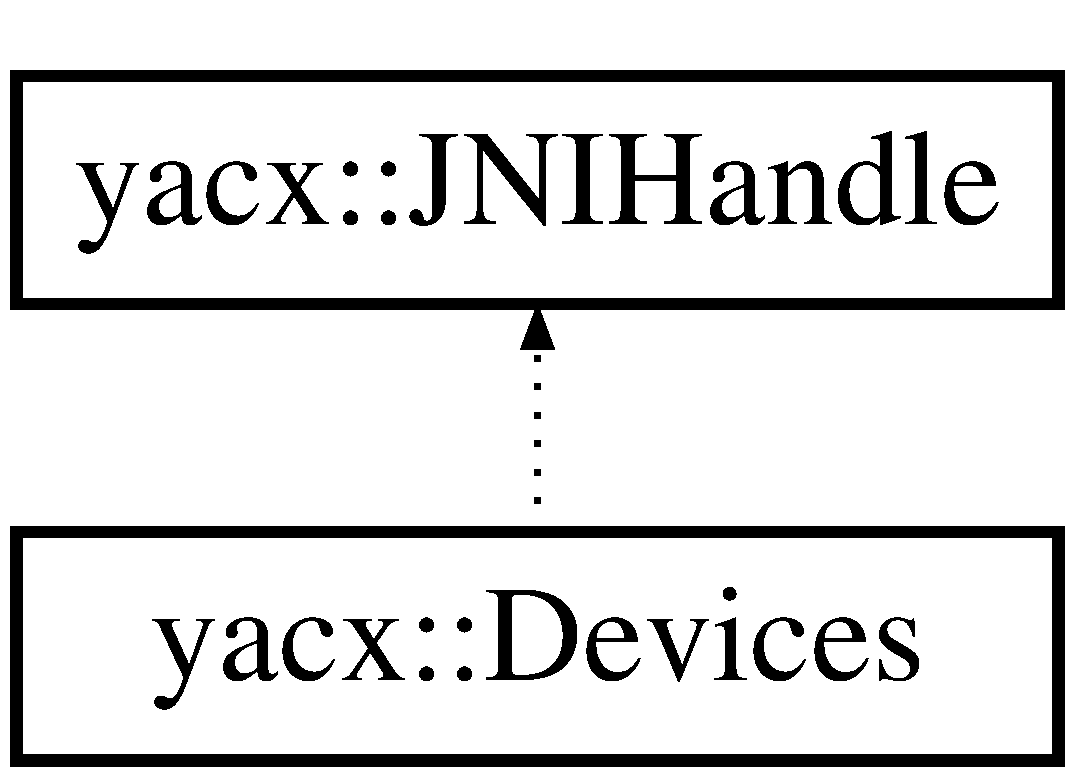
\includegraphics[height=2.000000cm]{classyacx_1_1_devices}
\end{center}
\end{figure}
\subsection*{Static Public Member Functions}
\begin{DoxyCompactItemize}
\item 
static \hyperlink{classyacx_1_1_device}{Device} \& \hyperlink{classyacx_1_1_devices_abaae9839d12e79117e2fb292ee0689fb}{find\+Device} ()
\item 
static \hyperlink{classyacx_1_1_device}{Device} \& \hyperlink{classyacx_1_1_devices_a89eb86ce0ad70dd0390375ee04f549f6}{find\+Device} (std\+::string name)
\item 
static \hyperlink{classyacx_1_1_device}{Device} \& \hyperlink{classyacx_1_1_devices_afbeb807ea9fac2ba0be9c4fa812c5243}{find\+Device\+By\+U\+U\+ID} (std\+::string uuid)
\item 
static std\+::vector$<$ \hyperlink{classyacx_1_1_device}{Device} $>$ \& \hyperlink{classyacx_1_1_devices_aa1a44930c265be1c6593af6c42cd9c12}{find\+Devices} ()
\item 
static std\+::vector$<$ \hyperlink{classyacx_1_1_device}{Device} $\ast$ $>$ \hyperlink{classyacx_1_1_devices_a274f530c0b46a7fcdd13d36b55330541}{find\+Devices} (std\+::function$<$ bool(\hyperlink{classyacx_1_1_device}{Device} \&)$>$ con)
\end{DoxyCompactItemize}


\subsection{Detailed Description}
\begin{Desc}
\item[Examples\+: ]\par
\hyperlink{example_matrix_multiply_8cpp-example}{example\+\_\+matrix\+\_\+multiply.\+cpp}, \hyperlink{example_program_8cpp-example}{example\+\_\+program.\+cpp}, and \hyperlink{example_saxpy_8cpp-example}{example\+\_\+saxpy.\+cpp}.\end{Desc}


\subsection{Member Function Documentation}
\mbox{\Hypertarget{classyacx_1_1_devices_abaae9839d12e79117e2fb292ee0689fb}\label{classyacx_1_1_devices_abaae9839d12e79117e2fb292ee0689fb}} 
\index{yacx\+::\+Devices@{yacx\+::\+Devices}!find\+Device@{find\+Device}}
\index{find\+Device@{find\+Device}!yacx\+::\+Devices@{yacx\+::\+Devices}}
\subsubsection{\texorpdfstring{find\+Device()}{findDevice()}\hspace{0.1cm}{\footnotesize\ttfamily [1/2]}}
{\footnotesize\ttfamily \hyperlink{classyacx_1_1_device}{Device} \& Devices\+::find\+Device (\begin{DoxyParamCaption}{ }\end{DoxyParamCaption})\hspace{0.3cm}{\ttfamily [static]}}

\begin{DoxyReturn}{Returns}
returns a \hyperlink{classyacx_1_1_device}{Device} with the first C\+U\+DA capable device it finds 
\end{DoxyReturn}
\mbox{\Hypertarget{classyacx_1_1_devices_a89eb86ce0ad70dd0390375ee04f549f6}\label{classyacx_1_1_devices_a89eb86ce0ad70dd0390375ee04f549f6}} 
\index{yacx\+::\+Devices@{yacx\+::\+Devices}!find\+Device@{find\+Device}}
\index{find\+Device@{find\+Device}!yacx\+::\+Devices@{yacx\+::\+Devices}}
\subsubsection{\texorpdfstring{find\+Device()}{findDevice()}\hspace{0.1cm}{\footnotesize\ttfamily [2/2]}}
{\footnotesize\ttfamily \hyperlink{classyacx_1_1_device}{Device} \& Devices\+::find\+Device (\begin{DoxyParamCaption}\item[{std\+::string}]{name }\end{DoxyParamCaption})\hspace{0.3cm}{\ttfamily [static]}}

\begin{DoxyReturn}{Returns}
returns a \hyperlink{classyacx_1_1_device}{Device} if a C\+U\+DA capable device with the identifier is available 
\end{DoxyReturn}

\begin{DoxyParams}{Parameters}
{\em name} & Name of the cuda device, e.\+g.\textquotesingle{}Tesla K20c\textquotesingle{} \\
\hline
\end{DoxyParams}
\mbox{\Hypertarget{classyacx_1_1_devices_afbeb807ea9fac2ba0be9c4fa812c5243}\label{classyacx_1_1_devices_afbeb807ea9fac2ba0be9c4fa812c5243}} 
\index{yacx\+::\+Devices@{yacx\+::\+Devices}!find\+Device\+By\+U\+U\+ID@{find\+Device\+By\+U\+U\+ID}}
\index{find\+Device\+By\+U\+U\+ID@{find\+Device\+By\+U\+U\+ID}!yacx\+::\+Devices@{yacx\+::\+Devices}}
\subsubsection{\texorpdfstring{find\+Device\+By\+U\+U\+I\+D()}{findDeviceByUUID()}}
{\footnotesize\ttfamily \hyperlink{classyacx_1_1_device}{Device} \& Devices\+::find\+Device\+By\+U\+U\+ID (\begin{DoxyParamCaption}\item[{std\+::string}]{uuid }\end{DoxyParamCaption})\hspace{0.3cm}{\ttfamily [static]}}

\begin{DoxyReturn}{Returns}
returns a \hyperlink{classyacx_1_1_device}{Device} if a C\+U\+DA capable device with the passed 16-\/byte U\+U\+ID as hexadecimal string 
\end{DoxyReturn}

\begin{DoxyParams}{Parameters}
{\em uuid} & U\+U\+ID of the cuda device \\
\hline
\end{DoxyParams}
\mbox{\Hypertarget{classyacx_1_1_devices_aa1a44930c265be1c6593af6c42cd9c12}\label{classyacx_1_1_devices_aa1a44930c265be1c6593af6c42cd9c12}} 
\index{yacx\+::\+Devices@{yacx\+::\+Devices}!find\+Devices@{find\+Devices}}
\index{find\+Devices@{find\+Devices}!yacx\+::\+Devices@{yacx\+::\+Devices}}
\subsubsection{\texorpdfstring{find\+Devices()}{findDevices()}\hspace{0.1cm}{\footnotesize\ttfamily [1/2]}}
{\footnotesize\ttfamily std\+::vector$<$ \hyperlink{classyacx_1_1_device}{Device} $>$ \& Devices\+::find\+Devices (\begin{DoxyParamCaption}{ }\end{DoxyParamCaption})\hspace{0.3cm}{\ttfamily [static]}}

\begin{DoxyReturn}{Returns}
vector with all C\+U\+D\+A-\/capable devices 
\end{DoxyReturn}
\mbox{\Hypertarget{classyacx_1_1_devices_a274f530c0b46a7fcdd13d36b55330541}\label{classyacx_1_1_devices_a274f530c0b46a7fcdd13d36b55330541}} 
\index{yacx\+::\+Devices@{yacx\+::\+Devices}!find\+Devices@{find\+Devices}}
\index{find\+Devices@{find\+Devices}!yacx\+::\+Devices@{yacx\+::\+Devices}}
\subsubsection{\texorpdfstring{find\+Devices()}{findDevices()}\hspace{0.1cm}{\footnotesize\ttfamily [2/2]}}
{\footnotesize\ttfamily std\+::vector$<$ \hyperlink{classyacx_1_1_device}{Device} $\ast$ $>$ Devices\+::find\+Devices (\begin{DoxyParamCaption}\item[{std\+::function$<$ bool(\hyperlink{classyacx_1_1_device}{Device} \&)$>$}]{con }\end{DoxyParamCaption})\hspace{0.3cm}{\ttfamily [static]}}

filters the devices satisfying passed condition 
\begin{DoxyParams}{Parameters}
{\em con} & condition for devices e.\+g.\textquotesingle{}\mbox{[}\mbox{]}(\hyperlink{classyacx_1_1_device}{Device}\& d)\{return d.\+total\+\_\+memory() $>$= 1024;\}\textquotesingle{} \\
\hline
\end{DoxyParams}
\begin{DoxyReturn}{Returns}
list of devices satisfying passed condition 
\end{DoxyReturn}


The documentation for this class was generated from the following files\+:\begin{DoxyCompactItemize}
\item 
include/yacx/Devices.\+hpp\item 
src/Devices.\+cpp\end{DoxyCompactItemize}

\hypertarget{structyacx_1_1detail_1_1dynop}{}\section{yacx\+:\+:detail\+:\+:dynop Struct Reference}
\label{structyacx_1_1detail_1_1dynop}\index{yacx\+::detail\+::dynop@{yacx\+::detail\+::dynop}}
\subsection*{Public Attributes}
\begin{DoxyCompactItemize}
\item 
\mbox{\Hypertarget{structyacx_1_1detail_1_1dynop_a369931b9091d6f11b403e59edc9deb02}\label{structyacx_1_1detail_1_1dynop_a369931b9091d6f11b403e59edc9deb02}} 
void($\ast$ {\bfseries op} )(void $\ast$$\ast$parameter)
\item 
\mbox{\Hypertarget{structyacx_1_1detail_1_1dynop_ab754a462a362da39f69a710e34851937}\label{structyacx_1_1detail_1_1dynop_ab754a462a362da39f69a710e34851937}} 
void $\ast$ {\bfseries libhandle}
\end{DoxyCompactItemize}


The documentation for this struct was generated from the following file\+:\begin{DoxyCompactItemize}
\item 
include/yacx/cexecutor/Libary\+Loader.\+hpp\end{DoxyCompactItemize}

\hypertarget{structyacx_1_1event_interval}{}\doxysection{yacx\+::event\+Interval Struct Reference}
\label{structyacx_1_1event_interval}\index{yacx::eventInterval@{yacx::eventInterval}}
\doxysubsection*{Public Member Functions}
\begin{DoxyCompactItemize}
\item 
\mbox{\Hypertarget{structyacx_1_1event_interval_a74213451bfa801df9117c6c91bfa9ca8}\label{structyacx_1_1event_interval_a74213451bfa801df9117c6c91bfa9ca8}} 
float {\bfseries elapsed} ()
\end{DoxyCompactItemize}
\doxysubsection*{Public Attributes}
\begin{DoxyCompactItemize}
\item 
\mbox{\Hypertarget{structyacx_1_1event_interval_a2bd8443ac3ab014c362febbb9efd43b1}\label{structyacx_1_1event_interval_a2bd8443ac3ab014c362febbb9efd43b1}} 
C\+Uevent {\bfseries start}
\item 
\mbox{\Hypertarget{structyacx_1_1event_interval_accea7d9c8870ccd71dca60a41f3349e3}\label{structyacx_1_1event_interval_accea7d9c8870ccd71dca60a41f3349e3}} 
C\+Uevent {\bfseries end}
\end{DoxyCompactItemize}


The documentation for this struct was generated from the following files\+:\begin{DoxyCompactItemize}
\item 
include/yacx/Kernel.\+hpp\item 
src/Kernel.\+cpp\end{DoxyCompactItemize}

\hypertarget{classyacx_1_1options_1_1_fast___math}{}\section{yacx\+:\+:options\+:\+:Fast\+\_\+\+Math Class Reference}
\label{classyacx_1_1options_1_1_fast___math}\index{yacx\+::options\+::\+Fast\+\_\+\+Math@{yacx\+::options\+::\+Fast\+\_\+\+Math}}
Inheritance diagram for yacx\+:\+:options\+:\+:Fast\+\_\+\+Math\+:\begin{figure}[H]
\begin{center}
\leavevmode
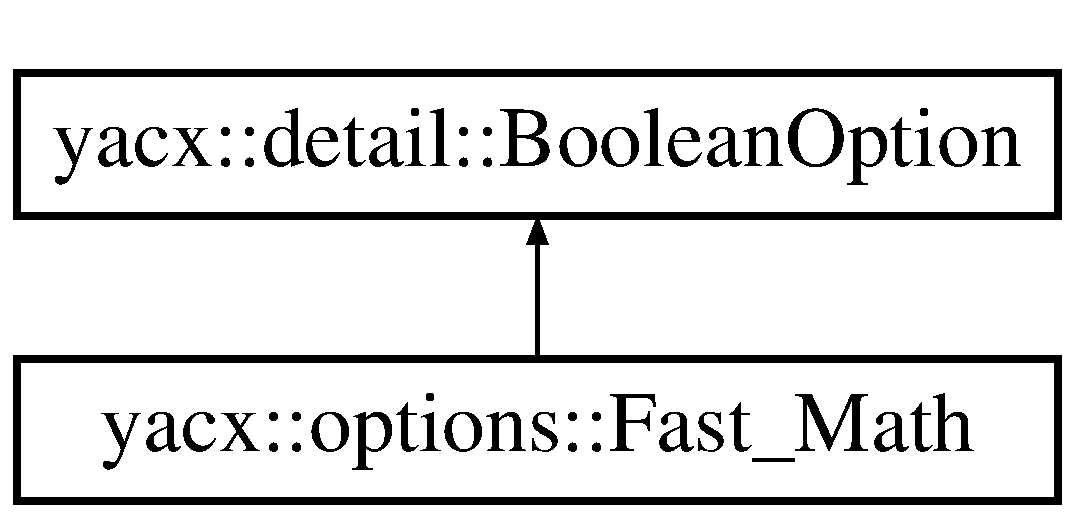
\includegraphics[height=2.000000cm]{classyacx_1_1options_1_1_fast___math}
\end{center}
\end{figure}
\subsection*{Public Member Functions}
\begin{DoxyCompactItemize}
\item 
\mbox{\Hypertarget{classyacx_1_1options_1_1_fast___math_ada740b2423739e7bda34770a529d5d91}\label{classyacx_1_1options_1_1_fast___math_ada740b2423739e7bda34770a529d5d91}} 
auto {\bfseries name} () const
\end{DoxyCompactItemize}


\subsection{Detailed Description}
\begin{Desc}
\item[Examples\+: ]\par
\hyperlink{docs_2options_construct_8cpp-example}{docs/options\+\_\+construct.\+cpp}.\end{Desc}


The documentation for this class was generated from the following file\+:\begin{DoxyCompactItemize}
\item 
include/yacx/Options.\+hpp\end{DoxyCompactItemize}

\hypertarget{classyacx_1_1options_1_1_f_m_a_d}{}\section{yacx\+:\+:options\+:\+:F\+M\+AD Class Reference}
\label{classyacx_1_1options_1_1_f_m_a_d}\index{yacx\+::options\+::\+F\+M\+AD@{yacx\+::options\+::\+F\+M\+AD}}
Inheritance diagram for yacx\+:\+:options\+:\+:F\+M\+AD\+:\begin{figure}[H]
\begin{center}
\leavevmode
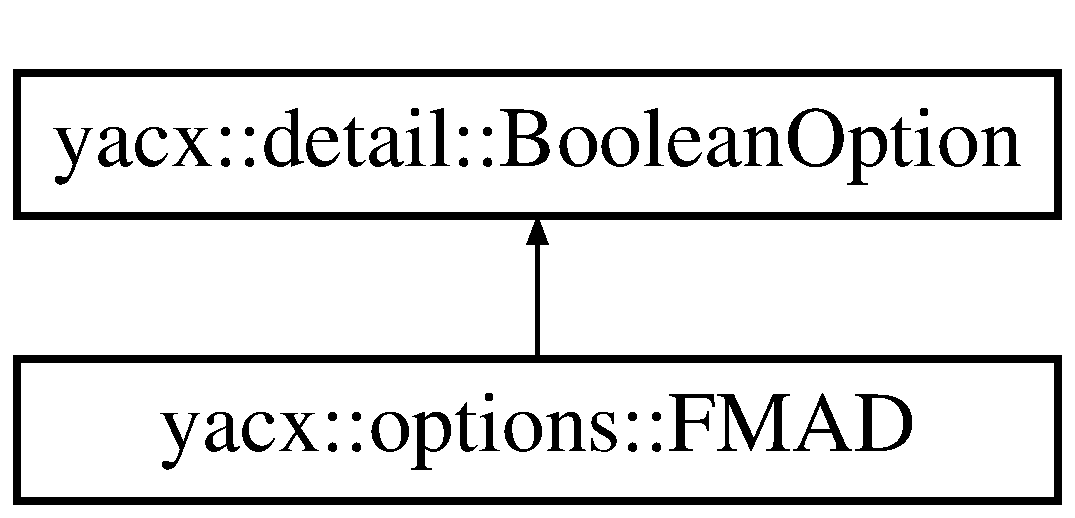
\includegraphics[height=2.000000cm]{classyacx_1_1options_1_1_f_m_a_d}
\end{center}
\end{figure}
\subsection*{Public Member Functions}
\begin{DoxyCompactItemize}
\item 
\mbox{\Hypertarget{classyacx_1_1options_1_1_f_m_a_d_a46c2300af4cd962af3585704094bcebb}\label{classyacx_1_1options_1_1_f_m_a_d_a46c2300af4cd962af3585704094bcebb}} 
auto {\bfseries name} () const
\end{DoxyCompactItemize}


\subsection{Detailed Description}
\begin{Desc}
\item[Examples\+: ]\par
\hyperlink{docs_2options_construct_8cpp-example}{docs/options\+\_\+construct.\+cpp}, and \hyperlink{example_program_8cpp-example}{example\+\_\+program.\+cpp}.\end{Desc}


The documentation for this class was generated from the following file\+:\begin{DoxyCompactItemize}
\item 
include/yacx/Options.\+hpp\end{DoxyCompactItemize}

\hypertarget{classyacx_1_1options_1_1_gpu_architecture}{}\doxysection{yacx\+::options\+::Gpu\+Architecture Class Reference}
\label{classyacx_1_1options_1_1_gpu_architecture}\index{yacx::options::GpuArchitecture@{yacx::options::GpuArchitecture}}
\doxysubsection*{Public Member Functions}
\begin{DoxyCompactItemize}
\item 
\mbox{\Hypertarget{classyacx_1_1options_1_1_gpu_architecture_a0baff902e638ca1173b1dc54801ed22a}\label{classyacx_1_1options_1_1_gpu_architecture_a0baff902e638ca1173b1dc54801ed22a}} 
{\bfseries Gpu\+Architecture} (int major, int minor)
\item 
\mbox{\Hypertarget{classyacx_1_1options_1_1_gpu_architecture_a26c7ac5e84db61aa65563dcd29f376b2}\label{classyacx_1_1options_1_1_gpu_architecture_a26c7ac5e84db61aa65563dcd29f376b2}} 
{\bfseries Gpu\+Architecture} (const \mbox{\hyperlink{classyacx_1_1_device}{yacx\+::\+Device}} \&device)
\item 
\mbox{\Hypertarget{classyacx_1_1options_1_1_gpu_architecture_a2407cc1ae8526a89987a82b5dcc7dda6}\label{classyacx_1_1options_1_1_gpu_architecture_a2407cc1ae8526a89987a82b5dcc7dda6}} 
auto {\bfseries name} () const
\item 
\mbox{\Hypertarget{classyacx_1_1options_1_1_gpu_architecture_aea50b543f6e12e9e32f9a977755269c7}\label{classyacx_1_1options_1_1_gpu_architecture_aea50b543f6e12e9e32f9a977755269c7}} 
auto \& {\bfseries value} () const
\end{DoxyCompactItemize}


\doxysubsection{Detailed Description}
\begin{Desc}
\item[Examples]\par
\mbox{\hyperlink{docs_2options_construct_8cpp-example}{docs/options\+\_\+construct.\+cpp}}, \mbox{\hyperlink{example_matrix_multiply_8cpp-example}{example\+\_\+matrix\+\_\+multiply.\+cpp}}, and \mbox{\hyperlink{example_program_8cpp-example}{example\+\_\+program.\+cpp}}.\end{Desc}


The documentation for this class was generated from the following file\+:\begin{DoxyCompactItemize}
\item 
include/yacx/Options.\+hpp\end{DoxyCompactItemize}

\hypertarget{classyacx_1_1_header}{}\section{yacx\+:\+:Header Class Reference}
\label{classyacx_1_1_header}\index{yacx\+::\+Header@{yacx\+::\+Header}}


Class to help import header files for \hyperlink{classyacx_1_1_source}{Source}.  




{\ttfamily \#include $<$Headers.\+hpp$>$}

\subsection*{Public Member Functions}
\begin{DoxyCompactItemize}
\item 
\hyperlink{classyacx_1_1_header_a359314e42c557b67be2ff790463f4f83}{Header} (const std\+::string \&path)
\item 
\mbox{\Hypertarget{classyacx_1_1_header_a76c4a02acb1d5fcc7689529c555aa578}\label{classyacx_1_1_header_a76c4a02acb1d5fcc7689529c555aa578}} 
const char $\ast$ {\bfseries name} () const
\item 
\mbox{\Hypertarget{classyacx_1_1_header_a4ff84507d1e3af182e612420d0a4f79e}\label{classyacx_1_1_header_a4ff84507d1e3af182e612420d0a4f79e}} 
size\+\_\+t {\bfseries length} () const
\item 
const char $\ast$ \hyperlink{classyacx_1_1_header_a6c16e8736a35b1644dfdf9caebee7ad5}{content} () const
\end{DoxyCompactItemize}


\subsection{Detailed Description}
Class to help import header files for \hyperlink{classyacx_1_1_source}{Source}. \begin{Desc}
\item[Examples\+: ]\par
\hyperlink{docs_2headers_8cpp-example}{docs/headers.\+cpp}, and \hyperlink{example_gauss_8cpp-example}{example\+\_\+gauss.\+cpp}.\end{Desc}


\subsection{Constructor \& Destructor Documentation}
\mbox{\Hypertarget{classyacx_1_1_header_a359314e42c557b67be2ff790463f4f83}\label{classyacx_1_1_header_a359314e42c557b67be2ff790463f4f83}} 
\index{yacx\+::\+Header@{yacx\+::\+Header}!Header@{Header}}
\index{Header@{Header}!yacx\+::\+Header@{yacx\+::\+Header}}
\subsubsection{\texorpdfstring{Header()}{Header()}}
{\footnotesize\ttfamily yacx\+::\+Header\+::\+Header (\begin{DoxyParamCaption}\item[{const std\+::string \&}]{path }\end{DoxyParamCaption})\hspace{0.3cm}{\ttfamily [inline]}, {\ttfamily [explicit]}}


\begin{DoxyParams}{Parameters}
{\em path} & relative path to header file \\
\hline
\end{DoxyParams}


\subsection{Member Function Documentation}
\mbox{\Hypertarget{classyacx_1_1_header_a6c16e8736a35b1644dfdf9caebee7ad5}\label{classyacx_1_1_header_a6c16e8736a35b1644dfdf9caebee7ad5}} 
\index{yacx\+::\+Header@{yacx\+::\+Header}!content@{content}}
\index{content@{content}!yacx\+::\+Header@{yacx\+::\+Header}}
\subsubsection{\texorpdfstring{content()}{content()}}
{\footnotesize\ttfamily const char$\ast$ yacx\+::\+Header\+::content (\begin{DoxyParamCaption}{ }\end{DoxyParamCaption}) const\hspace{0.3cm}{\ttfamily [inline]}}

\begin{DoxyReturn}{Returns}
c-\/style string of header content 
\end{DoxyReturn}


The documentation for this class was generated from the following file\+:\begin{DoxyCompactItemize}
\item 
include/yacx/Headers.\+hpp\end{DoxyCompactItemize}

\hypertarget{classyacx_1_1_headers}{}\section{yacx\+:\+:Headers Class Reference}
\label{classyacx_1_1_headers}\index{yacx\+::\+Headers@{yacx\+::\+Headers}}
Inheritance diagram for yacx\+:\+:Headers\+:\begin{figure}[H]
\begin{center}
\leavevmode
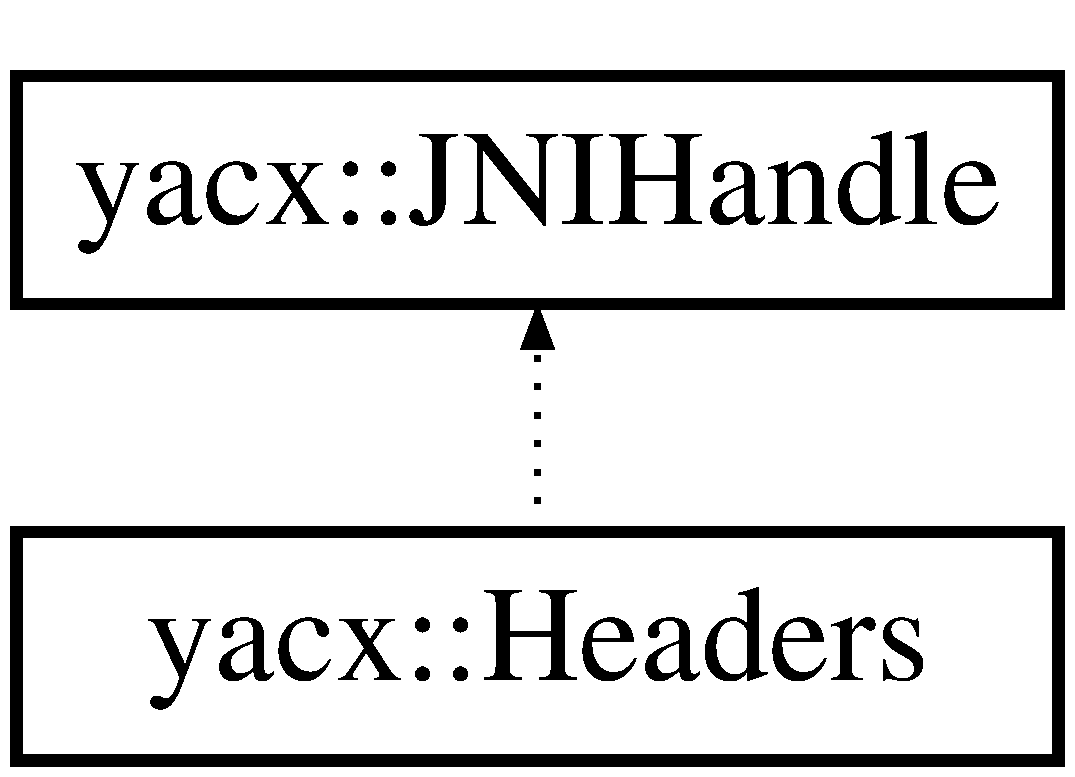
\includegraphics[height=2.000000cm]{classyacx_1_1_headers}
\end{center}
\end{figure}
\subsection*{Public Member Functions}
\begin{DoxyCompactItemize}
\item 
\hyperlink{classyacx_1_1_headers_ae04c7a09aac2e2417c7f5cb3410b011f}{Headers} (const \hyperlink{classyacx_1_1_header}{Header} \&header)
\item 
\hyperlink{classyacx_1_1_headers_af379ab4de8a97b9af8eff850987ce1d5}{Headers} (const std\+::string \&path)
\item 
\hyperlink{classyacx_1_1_headers_a4741fcbd110385f037be9091e20fd4a9}{Headers} (std\+::vector$<$ \hyperlink{classyacx_1_1_header}{Header} $>$ headers)
\item 
{\footnotesize template$<$typename T , typename... TS$>$ }\\\hyperlink{classyacx_1_1_headers_a2c695f86d62e478719878b37027e6cde}{Headers} (const T \&arg, const TS \&... args)
\item 
const char $\ast$$\ast$ \hyperlink{classyacx_1_1_headers_a80a31e958e7b1248bafdef6ce0c30c3c}{content} () const
\item 
const char $\ast$$\ast$ \hyperlink{classyacx_1_1_headers_aacf2017f07c4e9374a95facdf88863d7}{names} () const
\item 
size\+\_\+t \hyperlink{classyacx_1_1_headers_aed5718d17f7ab4e82b830708220fd00e}{num\+Headers} () const
\item 
void \hyperlink{classyacx_1_1_headers_a0428360b3ce224adc3a22bdbd486bfa0}{insert} (std\+::string const \&path)
\item 
void \hyperlink{classyacx_1_1_headers_a43251bcac778655f4b539e4e8f56e672}{insert} (\hyperlink{classyacx_1_1_header}{Header} header)
\end{DoxyCompactItemize}


\subsection{Detailed Description}
\begin{Desc}
\item[Examples\+: ]\par
\hyperlink{docs_2headers_8cpp-example}{docs/headers.\+cpp}, and \hyperlink{example_gauss_8cpp-example}{example\+\_\+gauss.\+cpp}.\end{Desc}


\subsection{Constructor \& Destructor Documentation}
\mbox{\Hypertarget{classyacx_1_1_headers_ae04c7a09aac2e2417c7f5cb3410b011f}\label{classyacx_1_1_headers_ae04c7a09aac2e2417c7f5cb3410b011f}} 
\index{yacx\+::\+Headers@{yacx\+::\+Headers}!Headers@{Headers}}
\index{Headers@{Headers}!yacx\+::\+Headers@{yacx\+::\+Headers}}
\subsubsection{\texorpdfstring{Headers()}{Headers()}\hspace{0.1cm}{\footnotesize\ttfamily [1/4]}}
{\footnotesize\ttfamily Headers\+::\+Headers (\begin{DoxyParamCaption}\item[{const \hyperlink{classyacx_1_1_header}{Header} \&}]{header }\end{DoxyParamCaption})\hspace{0.3cm}{\ttfamily [explicit]}}

constructs \hyperlink{classyacx_1_1_headers}{Headers} with \hyperlink{classyacx_1_1_header}{Header} 
\begin{DoxyParams}{Parameters}
{\em header} & \\
\hline
\end{DoxyParams}
\mbox{\Hypertarget{classyacx_1_1_headers_af379ab4de8a97b9af8eff850987ce1d5}\label{classyacx_1_1_headers_af379ab4de8a97b9af8eff850987ce1d5}} 
\index{yacx\+::\+Headers@{yacx\+::\+Headers}!Headers@{Headers}}
\index{Headers@{Headers}!yacx\+::\+Headers@{yacx\+::\+Headers}}
\subsubsection{\texorpdfstring{Headers()}{Headers()}\hspace{0.1cm}{\footnotesize\ttfamily [2/4]}}
{\footnotesize\ttfamily Headers\+::\+Headers (\begin{DoxyParamCaption}\item[{const std\+::string \&}]{path }\end{DoxyParamCaption})\hspace{0.3cm}{\ttfamily [explicit]}}

constructs \hyperlink{classyacx_1_1_headers}{Headers} with path to header file 
\begin{DoxyParams}{Parameters}
{\em path} & path to header file \\
\hline
\end{DoxyParams}
\mbox{\Hypertarget{classyacx_1_1_headers_a4741fcbd110385f037be9091e20fd4a9}\label{classyacx_1_1_headers_a4741fcbd110385f037be9091e20fd4a9}} 
\index{yacx\+::\+Headers@{yacx\+::\+Headers}!Headers@{Headers}}
\index{Headers@{Headers}!yacx\+::\+Headers@{yacx\+::\+Headers}}
\subsubsection{\texorpdfstring{Headers()}{Headers()}\hspace{0.1cm}{\footnotesize\ttfamily [3/4]}}
{\footnotesize\ttfamily Headers\+::\+Headers (\begin{DoxyParamCaption}\item[{std\+::vector$<$ \hyperlink{classyacx_1_1_header}{Header} $>$}]{headers }\end{DoxyParamCaption})\hspace{0.3cm}{\ttfamily [explicit]}}

constructs a header from a header vector 
\begin{DoxyParams}{Parameters}
{\em headers} & \\
\hline
\end{DoxyParams}
\mbox{\Hypertarget{classyacx_1_1_headers_a2c695f86d62e478719878b37027e6cde}\label{classyacx_1_1_headers_a2c695f86d62e478719878b37027e6cde}} 
\index{yacx\+::\+Headers@{yacx\+::\+Headers}!Headers@{Headers}}
\index{Headers@{Headers}!yacx\+::\+Headers@{yacx\+::\+Headers}}
\subsubsection{\texorpdfstring{Headers()}{Headers()}\hspace{0.1cm}{\footnotesize\ttfamily [4/4]}}
{\footnotesize\ttfamily template$<$typename T , typename... TS$>$ \\
Headers\+::\+Headers (\begin{DoxyParamCaption}\item[{const T \&}]{arg,  }\item[{const TS \&...}]{args }\end{DoxyParamCaption})}

constructs \hyperlink{classyacx_1_1_headers}{Headers} with a multiple \hyperlink{classyacx_1_1_header}{Header} or paths to header files 
\begin{DoxyTemplParams}{Template Parameters}
{\em T} & \hyperlink{classyacx_1_1_header}{Header}, std\+::string or char\mbox{[}\mbox{]} \\
\hline
{\em TS} & \hyperlink{classyacx_1_1_header}{Header}, std\+::string or char\mbox{[}\mbox{]} \\
\hline
\end{DoxyTemplParams}

\begin{DoxyParams}{Parameters}
{\em arg} & \hyperlink{classyacx_1_1_header}{Header} or Path to header file \\
\hline
{\em args} & \hyperlink{classyacx_1_1_header}{Header} or Path to header file \\
\hline
\end{DoxyParams}


\subsection{Member Function Documentation}
\mbox{\Hypertarget{classyacx_1_1_headers_a80a31e958e7b1248bafdef6ce0c30c3c}\label{classyacx_1_1_headers_a80a31e958e7b1248bafdef6ce0c30c3c}} 
\index{yacx\+::\+Headers@{yacx\+::\+Headers}!content@{content}}
\index{content@{content}!yacx\+::\+Headers@{yacx\+::\+Headers}}
\subsubsection{\texorpdfstring{content()}{content()}}
{\footnotesize\ttfamily const char $\ast$$\ast$ Headers\+::content (\begin{DoxyParamCaption}{ }\end{DoxyParamCaption}) const}

\begin{DoxyReturn}{Returns}
c-\/style string array of header file contents 
\end{DoxyReturn}
\mbox{\Hypertarget{classyacx_1_1_headers_a0428360b3ce224adc3a22bdbd486bfa0}\label{classyacx_1_1_headers_a0428360b3ce224adc3a22bdbd486bfa0}} 
\index{yacx\+::\+Headers@{yacx\+::\+Headers}!insert@{insert}}
\index{insert@{insert}!yacx\+::\+Headers@{yacx\+::\+Headers}}
\subsubsection{\texorpdfstring{insert()}{insert()}\hspace{0.1cm}{\footnotesize\ttfamily [1/2]}}
{\footnotesize\ttfamily void yacx\+::\+Headers\+::insert (\begin{DoxyParamCaption}\item[{std\+::string const \&}]{path }\end{DoxyParamCaption})\hspace{0.3cm}{\ttfamily [inline]}}

inserts \hyperlink{classyacx_1_1_header}{Header} 
\begin{DoxyParams}{Parameters}
{\em path} & path to header file \\
\hline
\end{DoxyParams}
\mbox{\Hypertarget{classyacx_1_1_headers_a43251bcac778655f4b539e4e8f56e672}\label{classyacx_1_1_headers_a43251bcac778655f4b539e4e8f56e672}} 
\index{yacx\+::\+Headers@{yacx\+::\+Headers}!insert@{insert}}
\index{insert@{insert}!yacx\+::\+Headers@{yacx\+::\+Headers}}
\subsubsection{\texorpdfstring{insert()}{insert()}\hspace{0.1cm}{\footnotesize\ttfamily [2/2]}}
{\footnotesize\ttfamily void yacx\+::\+Headers\+::insert (\begin{DoxyParamCaption}\item[{\hyperlink{classyacx_1_1_header}{Header}}]{header }\end{DoxyParamCaption})\hspace{0.3cm}{\ttfamily [inline]}}

inserts \hyperlink{classyacx_1_1_header}{Header} 
\begin{DoxyParams}{Parameters}
{\em header} & \\
\hline
\end{DoxyParams}
\mbox{\Hypertarget{classyacx_1_1_headers_aacf2017f07c4e9374a95facdf88863d7}\label{classyacx_1_1_headers_aacf2017f07c4e9374a95facdf88863d7}} 
\index{yacx\+::\+Headers@{yacx\+::\+Headers}!names@{names}}
\index{names@{names}!yacx\+::\+Headers@{yacx\+::\+Headers}}
\subsubsection{\texorpdfstring{names()}{names()}}
{\footnotesize\ttfamily const char $\ast$$\ast$ Headers\+::names (\begin{DoxyParamCaption}{ }\end{DoxyParamCaption}) const}

\begin{DoxyReturn}{Returns}
c-\/style string array of header file names 
\end{DoxyReturn}
\mbox{\Hypertarget{classyacx_1_1_headers_aed5718d17f7ab4e82b830708220fd00e}\label{classyacx_1_1_headers_aed5718d17f7ab4e82b830708220fd00e}} 
\index{yacx\+::\+Headers@{yacx\+::\+Headers}!num\+Headers@{num\+Headers}}
\index{num\+Headers@{num\+Headers}!yacx\+::\+Headers@{yacx\+::\+Headers}}
\subsubsection{\texorpdfstring{num\+Headers()}{numHeaders()}}
{\footnotesize\ttfamily size\+\_\+t yacx\+::\+Headers\+::num\+Headers (\begin{DoxyParamCaption}{ }\end{DoxyParamCaption}) const\hspace{0.3cm}{\ttfamily [inline]}}

\begin{DoxyReturn}{Returns}
number of header files 
\end{DoxyReturn}


The documentation for this class was generated from the following files\+:\begin{DoxyCompactItemize}
\item 
include/yacx/Headers.\+hpp\item 
src/Headers.\+cpp\end{DoxyCompactItemize}

\hypertarget{structyacx_1_1is__header}{}\doxysection{yacx\+::is\+\_\+header$<$ T $>$ Struct Template Reference}
\label{structyacx_1_1is__header}\index{yacx::is\_header$<$ T $>$@{yacx::is\_header$<$ T $>$}}


{\ttfamily \#include $<$Headers.\+hpp$>$}

Inheritance diagram for yacx\+::is\+\_\+header$<$ T $>$\+:\begin{figure}[H]
\begin{center}
\leavevmode
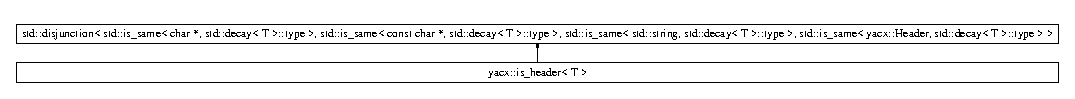
\includegraphics[height=0.886076cm]{structyacx_1_1is__header}
\end{center}
\end{figure}


\doxysubsection{Detailed Description}
\subsubsection*{template$<$typename T$>$\newline
struct yacx\+::is\+\_\+header$<$ T $>$}

checks if type is \mbox{\hyperlink{classyacx_1_1_header}{Header}} or can be casted to \mbox{\hyperlink{classyacx_1_1_header}{Header}} 
\begin{DoxyTemplParams}{Template Parameters}
{\em T} & type \\
\hline
\end{DoxyTemplParams}


The documentation for this struct was generated from the following file\+:\begin{DoxyCompactItemize}
\item 
include/yacx/Headers.\+hpp\end{DoxyCompactItemize}

\hypertarget{structyacx_1_1is__string}{}\doxysection{yacx\+::is\+\_\+string$<$ T $>$ Struct Template Reference}
\label{structyacx_1_1is__string}\index{yacx::is\_string$<$ T $>$@{yacx::is\_string$<$ T $>$}}
Inheritance diagram for yacx\+::is\+\_\+string$<$ T $>$\+:\begin{figure}[H]
\begin{center}
\leavevmode
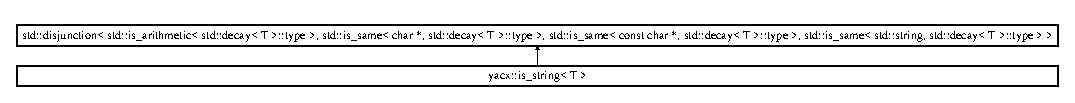
\includegraphics[height=0.929461cm]{structyacx_1_1is__string}
\end{center}
\end{figure}


The documentation for this struct was generated from the following file\+:\begin{DoxyCompactItemize}
\item 
include/yacx/util.\+hpp\end{DoxyCompactItemize}

\hypertarget{classyacx_1_1_j_n_i_handle}{}\doxysection{yacx\+::J\+N\+I\+Handle Class Reference}
\label{classyacx_1_1_j_n_i_handle}\index{yacx::JNIHandle@{yacx::JNIHandle}}
Inheritance diagram for yacx\+::J\+N\+I\+Handle\+:\begin{figure}[H]
\begin{center}
\leavevmode
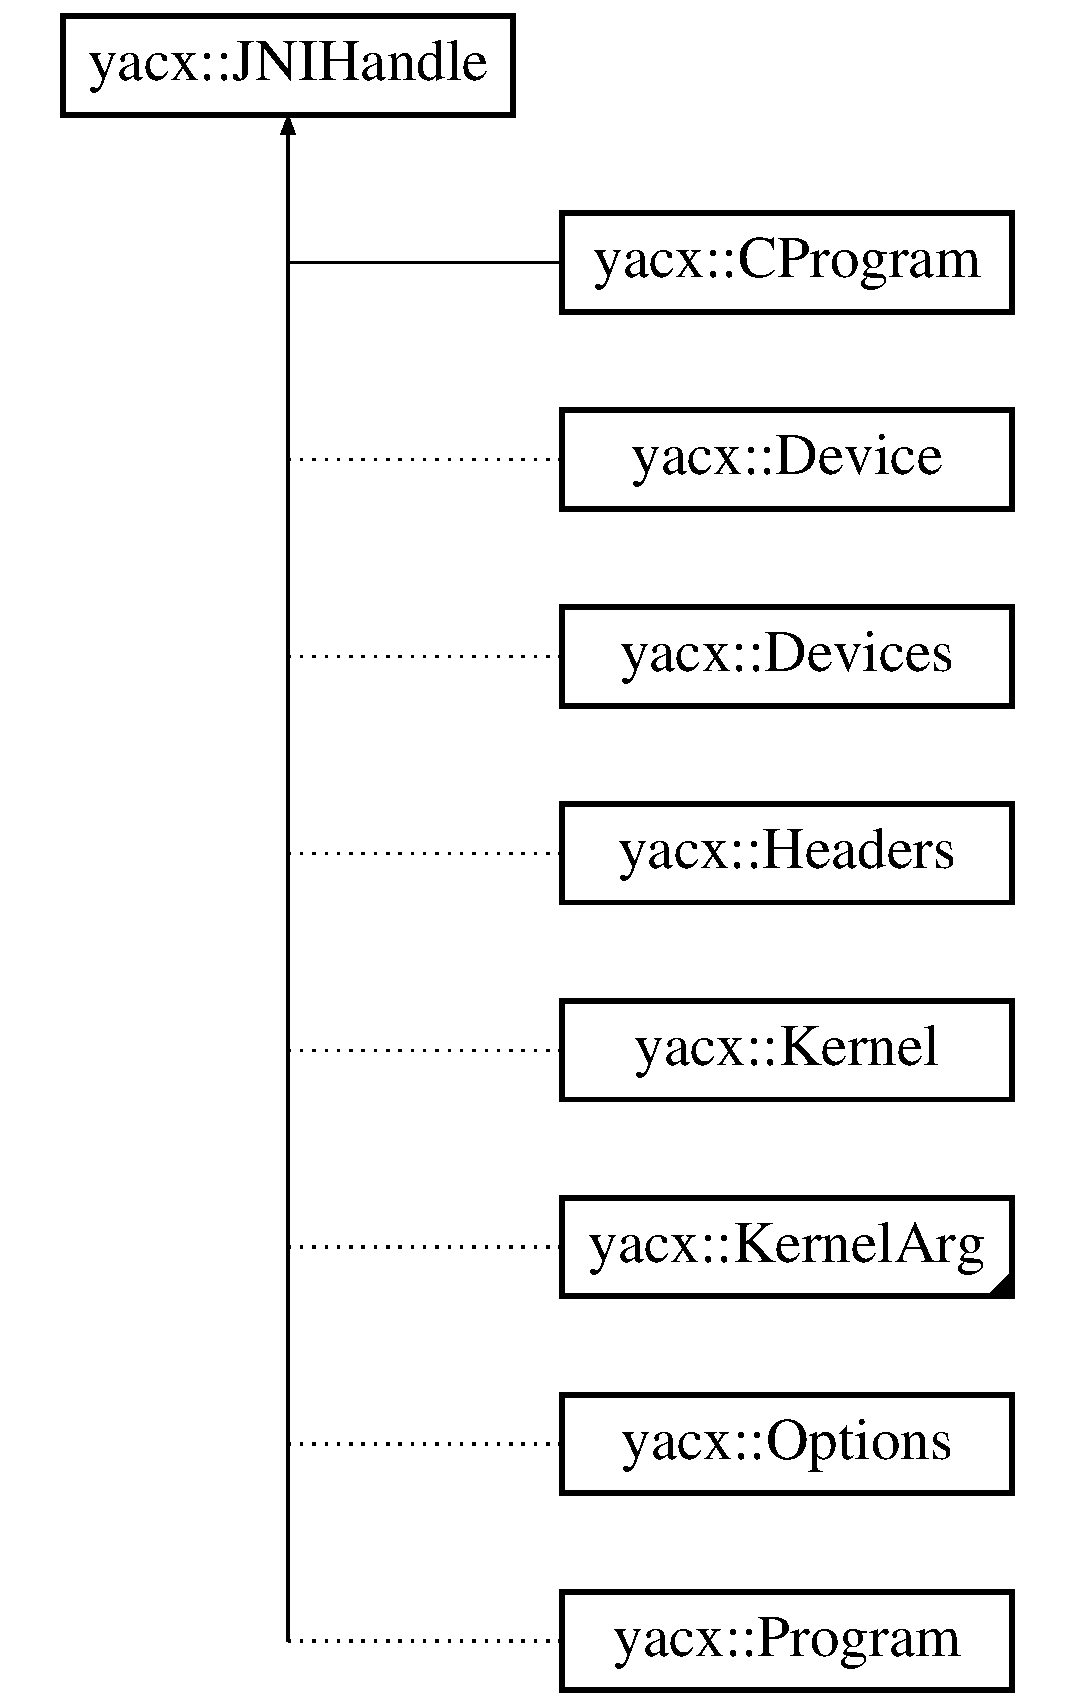
\includegraphics[height=9.000000cm]{classyacx_1_1_j_n_i_handle}
\end{center}
\end{figure}


The documentation for this class was generated from the following file\+:\begin{DoxyCompactItemize}
\item 
include/yacx/J\+N\+I\+Handle.\+hpp\end{DoxyCompactItemize}

\hypertarget{classyacx_1_1_kernel}{}\section{yacx\+:\+:Kernel Class Reference}
\label{classyacx_1_1_kernel}\index{yacx\+::\+Kernel@{yacx\+::\+Kernel}}


Class to help launch and configure a C\+U\+DA kernel.  




{\ttfamily \#include $<$Kernel.\+hpp$>$}

Inheritance diagram for yacx\+:\+:Kernel\+:\begin{figure}[H]
\begin{center}
\leavevmode
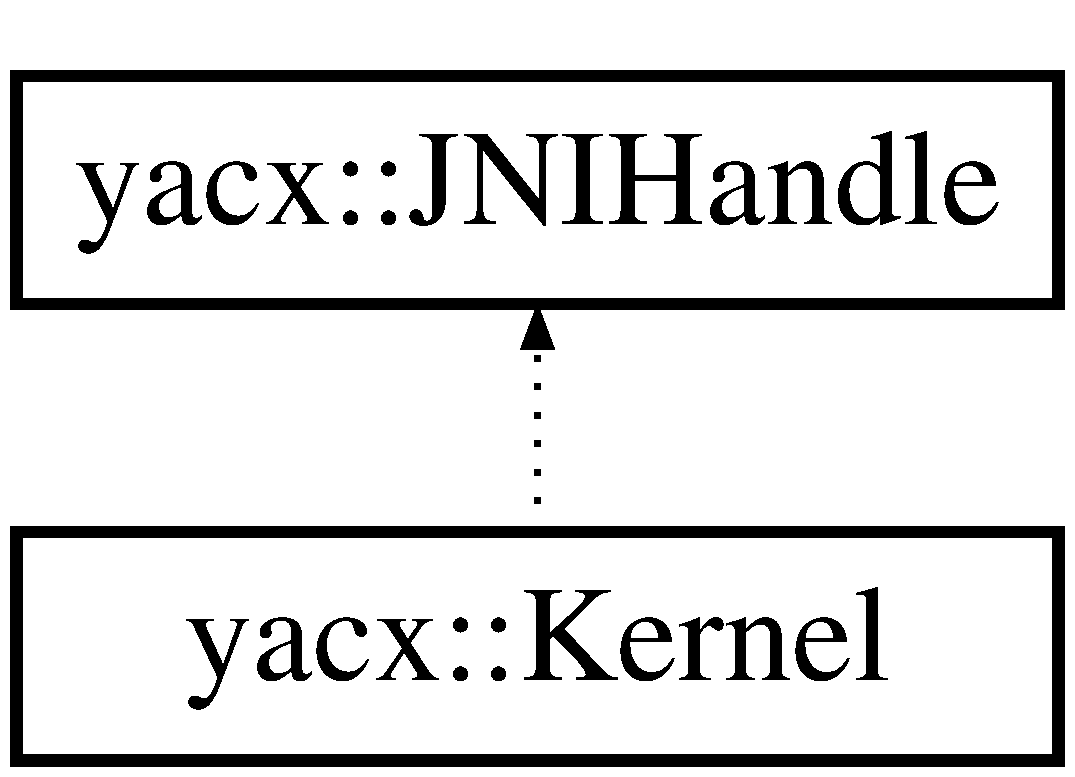
\includegraphics[height=2.000000cm]{classyacx_1_1_kernel}
\end{center}
\end{figure}
\subsection*{Public Member Functions}
\begin{DoxyCompactItemize}
\item 
\hyperlink{classyacx_1_1_kernel_af0bb713a4f07eb8304525731d0d1a9f9}{Kernel} (std\+::shared\+\_\+ptr$<$ char\mbox{[}$\,$\mbox{]}$>$ ptx, std\+::string demangled\+\_\+name)
\item 
\hyperlink{classyacx_1_1_kernel}{Kernel} \& \hyperlink{classyacx_1_1_kernel_abebec8a3f9a5dd82fc5df38304806c9d}{configure} (dim3 grid, dim3 block, unsigned int shared=0)
\item 
\hyperlink{structyacx_1_1_kernel_time_struct}{Kernel\+Time} \hyperlink{classyacx_1_1_kernel_a6daf13c0526e7746e0419697e7f861d7}{launch} (\hyperlink{classyacx_1_1_kernel_args}{Kernel\+Args} args, \hyperlink{classyacx_1_1_device}{Device} \&device=\hyperlink{classyacx_1_1_devices_abaae9839d12e79117e2fb292ee0689fb}{Devices\+::find\+Device}())
\item 
std\+::vector$<$ \hyperlink{structyacx_1_1_kernel_time_struct}{Kernel\+Time} $>$ \hyperlink{classyacx_1_1_kernel_a9fcd39747a74696078246d405e3a671f}{benchmark} (\hyperlink{classyacx_1_1_kernel_args}{Kernel\+Args} args, unsigned int executions, \hyperlink{classyacx_1_1_device}{Device} \&device=\hyperlink{classyacx_1_1_devices_abaae9839d12e79117e2fb292ee0689fb}{Devices\+::find\+Device}())
\end{DoxyCompactItemize}


\subsection{Detailed Description}
Class to help launch and configure a C\+U\+DA kernel. \begin{Desc}
\item[Examples\+: ]\par
\hyperlink{docs_2kernel_launch_8cpp-example}{docs/kernel\+\_\+launch.\+cpp}, \hyperlink{example_gauss_8cpp-example}{example\+\_\+gauss.\+cpp}, \hyperlink{example_matrix_multiply_8cpp-example}{example\+\_\+matrix\+\_\+multiply.\+cpp}, \hyperlink{example_saxpy_8cpp-example}{example\+\_\+saxpy.\+cpp}, and \hyperlink{example_template_8cpp-example}{example\+\_\+template.\+cpp}.\end{Desc}


\subsection{Constructor \& Destructor Documentation}
\mbox{\Hypertarget{classyacx_1_1_kernel_af0bb713a4f07eb8304525731d0d1a9f9}\label{classyacx_1_1_kernel_af0bb713a4f07eb8304525731d0d1a9f9}} 
\index{yacx\+::\+Kernel@{yacx\+::\+Kernel}!Kernel@{Kernel}}
\index{Kernel@{Kernel}!yacx\+::\+Kernel@{yacx\+::\+Kernel}}
\subsubsection{\texorpdfstring{Kernel()}{Kernel()}}
{\footnotesize\ttfamily Kernel\+::\+Kernel (\begin{DoxyParamCaption}\item[{std\+::shared\+\_\+ptr$<$ char\mbox{[}$\,$\mbox{]}$>$}]{ptx,  }\item[{std\+::string}]{demangled\+\_\+name }\end{DoxyParamCaption})}

create a \hyperlink{classyacx_1_1_kernel}{Kernel} based on a templated kernel string 
\begin{DoxyParams}{Parameters}
{\em ptx} & \\
\hline
{\em kernel\+\_\+name} & \\
\hline
{\em demangled\+\_\+name} & \\
\hline
\end{DoxyParams}


\subsection{Member Function Documentation}
\mbox{\Hypertarget{classyacx_1_1_kernel_a9fcd39747a74696078246d405e3a671f}\label{classyacx_1_1_kernel_a9fcd39747a74696078246d405e3a671f}} 
\index{yacx\+::\+Kernel@{yacx\+::\+Kernel}!benchmark@{benchmark}}
\index{benchmark@{benchmark}!yacx\+::\+Kernel@{yacx\+::\+Kernel}}
\subsubsection{\texorpdfstring{benchmark()}{benchmark()}}
{\footnotesize\ttfamily std\+::vector$<$ \hyperlink{structyacx_1_1_kernel_time_struct}{Kernel\+Time} $>$ Kernel\+::benchmark (\begin{DoxyParamCaption}\item[{\hyperlink{classyacx_1_1_kernel_args}{Kernel\+Args}}]{args,  }\item[{unsigned int}]{executions,  }\item[{\hyperlink{classyacx_1_1_device}{Device} \&}]{device = {\ttfamily \hyperlink{classyacx_1_1_devices_abaae9839d12e79117e2fb292ee0689fb}{Devices\+::find\+Device}()} }\end{DoxyParamCaption})}

benchmark a \hyperlink{classyacx_1_1_kernel}{Kernel} 
\begin{DoxyParams}{Parameters}
{\em kernel\+\_\+args} & \\
\hline
{\em number} & of executions \\
\hline
{\em device} & \\
\hline
\end{DoxyParams}
\begin{DoxyReturn}{Returns}
vector of Kernel\+Times for every execution 
\end{DoxyReturn}
\mbox{\Hypertarget{classyacx_1_1_kernel_abebec8a3f9a5dd82fc5df38304806c9d}\label{classyacx_1_1_kernel_abebec8a3f9a5dd82fc5df38304806c9d}} 
\index{yacx\+::\+Kernel@{yacx\+::\+Kernel}!configure@{configure}}
\index{configure@{configure}!yacx\+::\+Kernel@{yacx\+::\+Kernel}}
\subsubsection{\texorpdfstring{configure()}{configure()}}
{\footnotesize\ttfamily \hyperlink{classyacx_1_1_kernel}{Kernel} \& Kernel\+::configure (\begin{DoxyParamCaption}\item[{dim3}]{grid,  }\item[{dim3}]{block,  }\item[{unsigned int}]{shared = {\ttfamily 0} }\end{DoxyParamCaption})}


\begin{DoxyParams}{Parameters}
{\em grid} & vector of grid dimensions \\
\hline
{\em block} & vector of block dimensions \\
\hline
{\em shared} & amount of dynamic shared memory to allocate \\
\hline
\end{DoxyParams}
\begin{DoxyReturn}{Returns}
this (for method chaining) 
\end{DoxyReturn}
\mbox{\Hypertarget{classyacx_1_1_kernel_a6daf13c0526e7746e0419697e7f861d7}\label{classyacx_1_1_kernel_a6daf13c0526e7746e0419697e7f861d7}} 
\index{yacx\+::\+Kernel@{yacx\+::\+Kernel}!launch@{launch}}
\index{launch@{launch}!yacx\+::\+Kernel@{yacx\+::\+Kernel}}
\subsubsection{\texorpdfstring{launch()}{launch()}}
{\footnotesize\ttfamily \hyperlink{structyacx_1_1_kernel_time_struct}{Kernel\+Time} Kernel\+::launch (\begin{DoxyParamCaption}\item[{\hyperlink{classyacx_1_1_kernel_args}{Kernel\+Args}}]{args,  }\item[{\hyperlink{classyacx_1_1_device}{Device} \&}]{device = {\ttfamily \hyperlink{classyacx_1_1_devices_abaae9839d12e79117e2fb292ee0689fb}{Devices\+::find\+Device}()} }\end{DoxyParamCaption})}


\begin{DoxyParams}{Parameters}
{\em kernel\+\_\+args} & \\
\hline
\end{DoxyParams}
\begin{DoxyReturn}{Returns}
Kernel\+Time 
\end{DoxyReturn}


The documentation for this class was generated from the following files\+:\begin{DoxyCompactItemize}
\item 
include/yacx/Kernel.\+hpp\item 
src/Kernel.\+cpp\end{DoxyCompactItemize}

\hypertarget{classyacx_1_1_kernel_arg}{}\section{yacx\+:\+:Kernel\+Arg Class Reference}
\label{classyacx_1_1_kernel_arg}\index{yacx\+::\+Kernel\+Arg@{yacx\+::\+Kernel\+Arg}}
Inheritance diagram for yacx\+:\+:Kernel\+Arg\+:\begin{figure}[H]
\begin{center}
\leavevmode
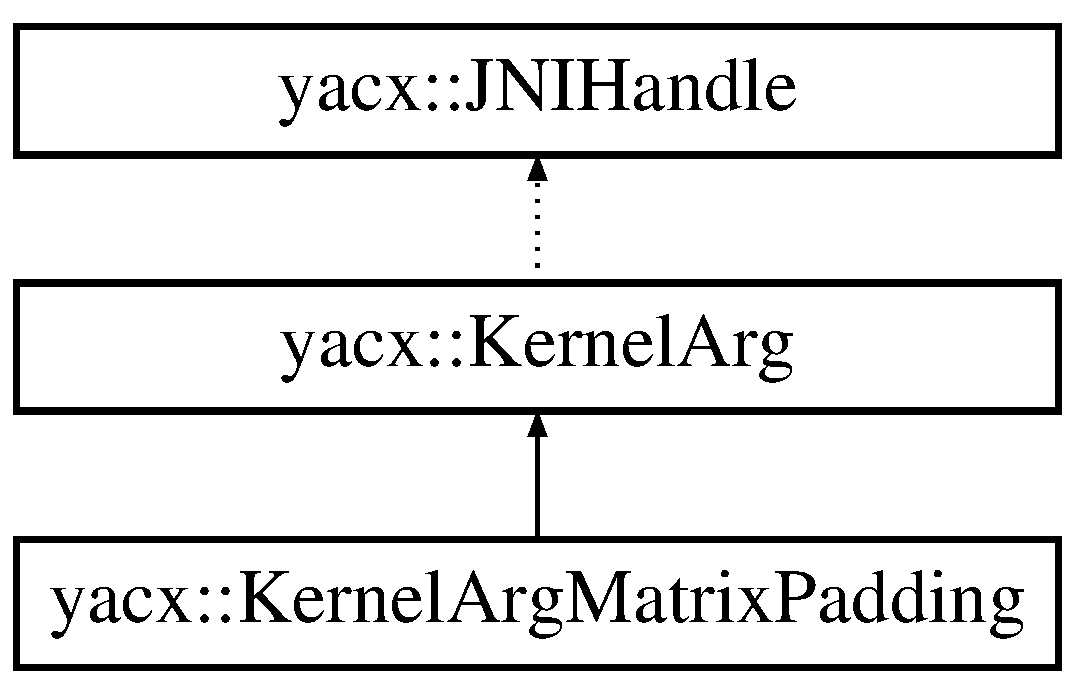
\includegraphics[height=3.000000cm]{classyacx_1_1_kernel_arg}
\end{center}
\end{figure}
\subsection*{Public Member Functions}
\begin{DoxyCompactItemize}
\item 
\hyperlink{classyacx_1_1_kernel_arg_a10f9f7255e69ef20c0cad5ed4e091c94}{Kernel\+Arg} (void $\ast$data, size\+\_\+t size, bool download=false, bool copy=true, bool upload=true)
\begin{DoxyCompactList}\small\item\em A constructor. \end{DoxyCompactList}\item 
\hyperlink{classyacx_1_1_kernel_arg_a52d84ba8210a080a8cb6e38d4b09981b}{Kernel\+Arg} (void $\ast$data)
\item 
const void $\ast$ \hyperlink{classyacx_1_1_kernel_arg_ae2151181887d6023f66c3198f71c4a47}{content} () const
\item 
C\+Udeviceptr \hyperlink{classyacx_1_1_kernel_arg_aac6471e5799fa67a873f8736a9f9b5d5}{deviceptr} ()
\item 
\mbox{\Hypertarget{classyacx_1_1_kernel_arg_a5dfe915de60f093466e9313c136aee4a}\label{classyacx_1_1_kernel_arg_a5dfe915de60f093466e9313c136aee4a}} 
void \hyperlink{classyacx_1_1_kernel_arg_a5dfe915de60f093466e9313c136aee4a}{malloc} ()
\begin{DoxyCompactList}\small\item\em mallocs data on device \end{DoxyCompactList}\item 
void \hyperlink{classyacx_1_1_kernel_arg_a28c10b39d51a27d30e0f3e60b6aea41e}{upload\+Async} (C\+Ustream stream)
\item 
void \hyperlink{classyacx_1_1_kernel_arg_abf4eb27a411c5f7396865398f4082441}{download\+Async} (C\+Ustream stream)
\item 
void \hyperlink{classyacx_1_1_kernel_arg_a0b58bafa9bb3b438a3a9e1f653ac53eb}{download\+Async} (void $\ast$hdata, C\+Ustream stream)
\item 
\mbox{\Hypertarget{classyacx_1_1_kernel_arg_a2cffe32c3423fbbcfa54223103995b97}\label{classyacx_1_1_kernel_arg_a2cffe32c3423fbbcfa54223103995b97}} 
void \hyperlink{classyacx_1_1_kernel_arg_a2cffe32c3423fbbcfa54223103995b97}{free} ()
\begin{DoxyCompactList}\small\item\em frees allocated data on device \end{DoxyCompactList}\item 
\mbox{\Hypertarget{classyacx_1_1_kernel_arg_a728724fe0e5bbbc6de98923dbb11d3b0}\label{classyacx_1_1_kernel_arg_a728724fe0e5bbbc6de98923dbb11d3b0}} 
size\+\_\+t {\bfseries size} () const
\item 
\mbox{\Hypertarget{classyacx_1_1_kernel_arg_a2a1b003ed2124e1a446c6f4317b2217d}\label{classyacx_1_1_kernel_arg_a2a1b003ed2124e1a446c6f4317b2217d}} 
bool {\bfseries is\+Download} () const
\item 
\mbox{\Hypertarget{classyacx_1_1_kernel_arg_abdc0850586cdd62d3c4a86b1de190910}\label{classyacx_1_1_kernel_arg_abdc0850586cdd62d3c4a86b1de190910}} 
void {\bfseries set\+Download} (bool download)
\item 
\mbox{\Hypertarget{classyacx_1_1_kernel_arg_a10e211a6138fe61e256876e97e503a6b}\label{classyacx_1_1_kernel_arg_a10e211a6138fe61e256876e97e503a6b}} 
bool {\bfseries is\+Copy} () const
\item 
\mbox{\Hypertarget{classyacx_1_1_kernel_arg_a46d69a02ec09adbbbcdb536a1ce2a2ba}\label{classyacx_1_1_kernel_arg_a46d69a02ec09adbbbcdb536a1ce2a2ba}} 
void {\bfseries set\+Copy} (bool copy)
\end{DoxyCompactItemize}
\subsection*{Protected Attributes}
\begin{DoxyCompactItemize}
\item 
\mbox{\Hypertarget{classyacx_1_1_kernel_arg_aa5674ed7907ccae1b0af176fbbfa6454}\label{classyacx_1_1_kernel_arg_aa5674ed7907ccae1b0af176fbbfa6454}} 
const void $\ast$ {\bfseries m\+\_\+hdata}
\item 
\mbox{\Hypertarget{classyacx_1_1_kernel_arg_a21c0cabef64800bafe49f588d16beaa6}\label{classyacx_1_1_kernel_arg_a21c0cabef64800bafe49f588d16beaa6}} 
C\+Udeviceptr {\bfseries m\+\_\+ddata}
\item 
\mbox{\Hypertarget{classyacx_1_1_kernel_arg_a6e76bbe8fa15c20702fd7b1d052440fa}\label{classyacx_1_1_kernel_arg_a6e76bbe8fa15c20702fd7b1d052440fa}} 
std\+::shared\+\_\+ptr$<$ \hyperlink{classyacx_1_1detail_1_1_data_copy}{detail\+::\+Data\+Copy} $>$ {\bfseries m\+\_\+data\+Copy}
\end{DoxyCompactItemize}
\subsection*{Friends}
\begin{DoxyCompactItemize}
\item 
\mbox{\Hypertarget{classyacx_1_1_kernel_arg_a487e05f65911a91df819064237f418b8}\label{classyacx_1_1_kernel_arg_a487e05f65911a91df819064237f418b8}} 
class {\bfseries Kernel\+Args}
\end{DoxyCompactItemize}


\subsection{Detailed Description}
\begin{Desc}
\item[Examples\+: ]\par
\hyperlink{docs_2kernel_args_8cpp-example}{docs/kernel\+\_\+args.\+cpp}, \hyperlink{docs_2kernel_launch_8cpp-example}{docs/kernel\+\_\+launch.\+cpp}, \hyperlink{example_gauss_8cpp-example}{example\+\_\+gauss.\+cpp}, \hyperlink{example_matrix_multiply_8cpp-example}{example\+\_\+matrix\+\_\+multiply.\+cpp}, \hyperlink{example_program_8cpp-example}{example\+\_\+program.\+cpp}, \hyperlink{example_saxpy_8cpp-example}{example\+\_\+saxpy.\+cpp}, and \hyperlink{example_template_8cpp-example}{example\+\_\+template.\+cpp}.\end{Desc}


\subsection{Constructor \& Destructor Documentation}
\mbox{\Hypertarget{classyacx_1_1_kernel_arg_a10f9f7255e69ef20c0cad5ed4e091c94}\label{classyacx_1_1_kernel_arg_a10f9f7255e69ef20c0cad5ed4e091c94}} 
\index{yacx\+::\+Kernel\+Arg@{yacx\+::\+Kernel\+Arg}!Kernel\+Arg@{Kernel\+Arg}}
\index{Kernel\+Arg@{Kernel\+Arg}!yacx\+::\+Kernel\+Arg@{yacx\+::\+Kernel\+Arg}}
\subsubsection{\texorpdfstring{Kernel\+Arg()}{KernelArg()}\hspace{0.1cm}{\footnotesize\ttfamily [1/2]}}
{\footnotesize\ttfamily Kernel\+Arg\+::\+Kernel\+Arg (\begin{DoxyParamCaption}\item[{void $\ast$}]{data,  }\item[{size\+\_\+t}]{size,  }\item[{bool}]{download = {\ttfamily false},  }\item[{bool}]{copy = {\ttfamily true},  }\item[{bool}]{upload = {\ttfamily true} }\end{DoxyParamCaption})}



A constructor. 


\begin{DoxyParams}{Parameters}
{\em data} & pointer to argument for kernel function \\
\hline
{\em size} & size of argument in bytes \\
\hline
{\em download} & copy the results from device to host after kernel execution \\
\hline
{\em copy} & copy the results to the device \\
\hline
{\em upload} & allocate the argument on the device (not necessary for basic types, e.\+g. int) \\
\hline
\end{DoxyParams}
\mbox{\Hypertarget{classyacx_1_1_kernel_arg_a52d84ba8210a080a8cb6e38d4b09981b}\label{classyacx_1_1_kernel_arg_a52d84ba8210a080a8cb6e38d4b09981b}} 
\index{yacx\+::\+Kernel\+Arg@{yacx\+::\+Kernel\+Arg}!Kernel\+Arg@{Kernel\+Arg}}
\index{Kernel\+Arg@{Kernel\+Arg}!yacx\+::\+Kernel\+Arg@{yacx\+::\+Kernel\+Arg}}
\subsubsection{\texorpdfstring{Kernel\+Arg()}{KernelArg()}\hspace{0.1cm}{\footnotesize\ttfamily [2/2]}}
{\footnotesize\ttfamily yacx\+::\+Kernel\+Arg\+::\+Kernel\+Arg (\begin{DoxyParamCaption}\item[{void $\ast$}]{data }\end{DoxyParamCaption})\hspace{0.3cm}{\ttfamily [inline]}, {\ttfamily [explicit]}}

A constructor for basic types, e.\+g. int 
\begin{DoxyParams}{Parameters}
{\em data} & pointer to argument for kernel function \\
\hline
\end{DoxyParams}


\subsection{Member Function Documentation}
\mbox{\Hypertarget{classyacx_1_1_kernel_arg_ae2151181887d6023f66c3198f71c4a47}\label{classyacx_1_1_kernel_arg_ae2151181887d6023f66c3198f71c4a47}} 
\index{yacx\+::\+Kernel\+Arg@{yacx\+::\+Kernel\+Arg}!content@{content}}
\index{content@{content}!yacx\+::\+Kernel\+Arg@{yacx\+::\+Kernel\+Arg}}
\subsubsection{\texorpdfstring{content()}{content()}}
{\footnotesize\ttfamily const void $\ast$ Kernel\+Arg\+::content (\begin{DoxyParamCaption}{ }\end{DoxyParamCaption}) const}

\begin{DoxyReturn}{Returns}
pointer to host data 
\end{DoxyReturn}
\mbox{\Hypertarget{classyacx_1_1_kernel_arg_aac6471e5799fa67a873f8736a9f9b5d5}\label{classyacx_1_1_kernel_arg_aac6471e5799fa67a873f8736a9f9b5d5}} 
\index{yacx\+::\+Kernel\+Arg@{yacx\+::\+Kernel\+Arg}!deviceptr@{deviceptr}}
\index{deviceptr@{deviceptr}!yacx\+::\+Kernel\+Arg@{yacx\+::\+Kernel\+Arg}}
\subsubsection{\texorpdfstring{deviceptr()}{deviceptr()}}
{\footnotesize\ttfamily C\+Udeviceptr yacx\+::\+Kernel\+Arg\+::deviceptr (\begin{DoxyParamCaption}{ }\end{DoxyParamCaption})\hspace{0.3cm}{\ttfamily [inline]}}

\begin{DoxyReturn}{Returns}
pointer to device data 
\end{DoxyReturn}
\mbox{\Hypertarget{classyacx_1_1_kernel_arg_abf4eb27a411c5f7396865398f4082441}\label{classyacx_1_1_kernel_arg_abf4eb27a411c5f7396865398f4082441}} 
\index{yacx\+::\+Kernel\+Arg@{yacx\+::\+Kernel\+Arg}!download\+Async@{download\+Async}}
\index{download\+Async@{download\+Async}!yacx\+::\+Kernel\+Arg@{yacx\+::\+Kernel\+Arg}}
\subsubsection{\texorpdfstring{download\+Async()}{downloadAsync()}\hspace{0.1cm}{\footnotesize\ttfamily [1/2]}}
{\footnotesize\ttfamily void yacx\+::\+Kernel\+Arg\+::download\+Async (\begin{DoxyParamCaption}\item[{C\+Ustream}]{stream }\end{DoxyParamCaption})\hspace{0.3cm}{\ttfamily [inline]}}

downloads data to host 
\begin{DoxyParams}{Parameters}
{\em stream} & to enqueue operations \\
\hline
\end{DoxyParams}
\mbox{\Hypertarget{classyacx_1_1_kernel_arg_a0b58bafa9bb3b438a3a9e1f653ac53eb}\label{classyacx_1_1_kernel_arg_a0b58bafa9bb3b438a3a9e1f653ac53eb}} 
\index{yacx\+::\+Kernel\+Arg@{yacx\+::\+Kernel\+Arg}!download\+Async@{download\+Async}}
\index{download\+Async@{download\+Async}!yacx\+::\+Kernel\+Arg@{yacx\+::\+Kernel\+Arg}}
\subsubsection{\texorpdfstring{download\+Async()}{downloadAsync()}\hspace{0.1cm}{\footnotesize\ttfamily [2/2]}}
{\footnotesize\ttfamily void Kernel\+Arg\+::download\+Async (\begin{DoxyParamCaption}\item[{void $\ast$}]{hdata,  }\item[{C\+Ustream}]{stream }\end{DoxyParamCaption})}

downloads data to host 
\begin{DoxyParams}{Parameters}
{\em hdata} & pointer to host memory for the downloaded data \\
\hline
{\em stream} & to enqueue operations \\
\hline
\end{DoxyParams}
\mbox{\Hypertarget{classyacx_1_1_kernel_arg_a28c10b39d51a27d30e0f3e60b6aea41e}\label{classyacx_1_1_kernel_arg_a28c10b39d51a27d30e0f3e60b6aea41e}} 
\index{yacx\+::\+Kernel\+Arg@{yacx\+::\+Kernel\+Arg}!upload\+Async@{upload\+Async}}
\index{upload\+Async@{upload\+Async}!yacx\+::\+Kernel\+Arg@{yacx\+::\+Kernel\+Arg}}
\subsubsection{\texorpdfstring{upload\+Async()}{uploadAsync()}}
{\footnotesize\ttfamily void Kernel\+Arg\+::upload\+Async (\begin{DoxyParamCaption}\item[{C\+Ustream}]{stream }\end{DoxyParamCaption})}

uploads data to device 
\begin{DoxyParams}{Parameters}
{\em stream} & to enqueue operations \\
\hline
\end{DoxyParams}


The documentation for this class was generated from the following files\+:\begin{DoxyCompactItemize}
\item 
include/yacx/Kernel\+Args.\+hpp\item 
src/Kernel\+Arg.\+cpp\end{DoxyCompactItemize}

\hypertarget{classyacx_1_1_kernel_arg_matrix_padding}{}\section{yacx\+:\+:Kernel\+Arg\+Matrix\+Padding Class Reference}
\label{classyacx_1_1_kernel_arg_matrix_padding}\index{yacx\+::\+Kernel\+Arg\+Matrix\+Padding@{yacx\+::\+Kernel\+Arg\+Matrix\+Padding}}
Inheritance diagram for yacx\+:\+:Kernel\+Arg\+Matrix\+Padding\+:\begin{figure}[H]
\begin{center}
\leavevmode
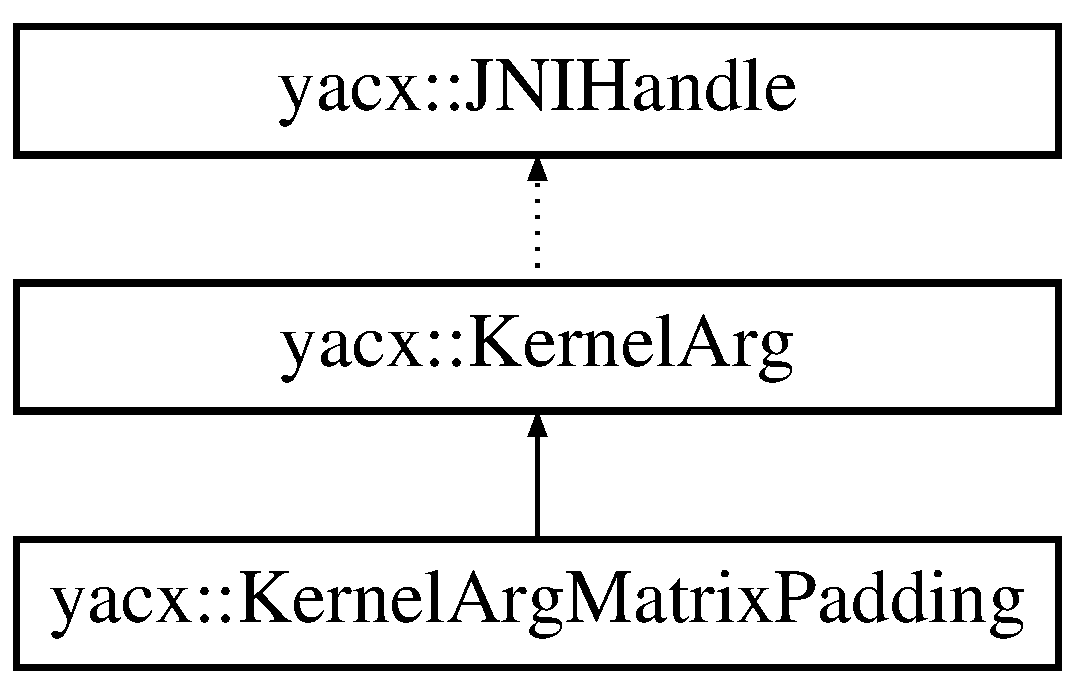
\includegraphics[height=3.000000cm]{classyacx_1_1_kernel_arg_matrix_padding}
\end{center}
\end{figure}
\subsection*{Public Member Functions}
\begin{DoxyCompactItemize}
\item 
\hyperlink{classyacx_1_1_kernel_arg_matrix_padding_ae1deb41319073ffa43589668baa7de63}{Kernel\+Arg\+Matrix\+Padding} (void $\ast$data, size\+\_\+t size, bool download, int element\+Size, unsigned int padding\+Value, int src\+\_\+rows, int src\+\_\+columns, int dst\+\_\+rows, int dst\+\_\+columns)
\begin{DoxyCompactList}\small\item\em A constructor. \end{DoxyCompactList}\end{DoxyCompactItemize}
\subsection*{Additional Inherited Members}


\subsection{Constructor \& Destructor Documentation}
\mbox{\Hypertarget{classyacx_1_1_kernel_arg_matrix_padding_ae1deb41319073ffa43589668baa7de63}\label{classyacx_1_1_kernel_arg_matrix_padding_ae1deb41319073ffa43589668baa7de63}} 
\index{yacx\+::\+Kernel\+Arg\+Matrix\+Padding@{yacx\+::\+Kernel\+Arg\+Matrix\+Padding}!Kernel\+Arg\+Matrix\+Padding@{Kernel\+Arg\+Matrix\+Padding}}
\index{Kernel\+Arg\+Matrix\+Padding@{Kernel\+Arg\+Matrix\+Padding}!yacx\+::\+Kernel\+Arg\+Matrix\+Padding@{yacx\+::\+Kernel\+Arg\+Matrix\+Padding}}
\subsubsection{\texorpdfstring{Kernel\+Arg\+Matrix\+Padding()}{KernelArgMatrixPadding()}}
{\footnotesize\ttfamily Kernel\+Arg\+Matrix\+Padding\+::\+Kernel\+Arg\+Matrix\+Padding (\begin{DoxyParamCaption}\item[{void $\ast$}]{data,  }\item[{size\+\_\+t}]{size,  }\item[{bool}]{download,  }\item[{int}]{element\+Size,  }\item[{unsigned int}]{padding\+Value,  }\item[{int}]{src\+\_\+rows,  }\item[{int}]{src\+\_\+columns,  }\item[{int}]{dst\+\_\+rows,  }\item[{int}]{dst\+\_\+columns }\end{DoxyParamCaption})}



A constructor. 


\begin{DoxyParams}{Parameters}
{\em data} & pointer to argument for kernel function \\
\hline
{\em size} & size of argument in bytes \\
\hline
{\em download} & copy the results from device to host after kernel execution types, e.\+g. int) \\
\hline
{\em element\+Size} & size of each element of the matrix in bytes \\
\hline
{\em padding\+Value} & value to fill up additional rows and columns \\
\hline
{\em src\+\_\+rows} & number of rows of current matrix without padding \\
\hline
{\em src\+\_\+columns} & number of columns of currentmatrix without padding \\
\hline
{\em dst\+\_\+rows} & number of rows for new matrix with padding \\
\hline
{\em dst\+\_\+columns} & number of columns for new matrix with padding \\
\hline
\end{DoxyParams}


The documentation for this class was generated from the following files\+:\begin{DoxyCompactItemize}
\item 
include/yacx/Kernel\+Args.\+hpp\item 
src/Kernel\+Arg.\+cpp\end{DoxyCompactItemize}

\hypertarget{classyacx_1_1_kernel_args}{}\doxysection{yacx\+::Kernel\+Args Class Reference}
\label{classyacx_1_1_kernel_args}\index{yacx::KernelArgs@{yacx::KernelArgs}}
\doxysubsection*{Public Member Functions}
\begin{DoxyCompactItemize}
\item 
\mbox{\Hypertarget{classyacx_1_1_kernel_args_a856a48b3aca3da86e811bc25bdd9b6e5}\label{classyacx_1_1_kernel_args_a856a48b3aca3da86e811bc25bdd9b6e5}} 
{\bfseries Kernel\+Args} (std\+::vector$<$ \mbox{\hyperlink{classyacx_1_1_kernel_arg}{Kernel\+Arg}} $>$ args)
\item 
\mbox{\Hypertarget{classyacx_1_1_kernel_args_a82b803d06c23a66348ee393d6b9ca5af}\label{classyacx_1_1_kernel_args_a82b803d06c23a66348ee393d6b9ca5af}} 
void {\bfseries malloc} ()
\item 
\mbox{\Hypertarget{classyacx_1_1_kernel_args_ada0a5d61939cab45bee8fe1e58dbef98}\label{classyacx_1_1_kernel_args_ada0a5d61939cab45bee8fe1e58dbef98}} 
void {\bfseries upload\+Async} (C\+Ustream stream)
\item 
\mbox{\Hypertarget{classyacx_1_1_kernel_args_a7b94f1458c8dab73e0bfe16b62d713fe}\label{classyacx_1_1_kernel_args_a7b94f1458c8dab73e0bfe16b62d713fe}} 
void {\bfseries download\+Async} (C\+Ustream stream)
\item 
\mbox{\Hypertarget{classyacx_1_1_kernel_args_a8dccbadb58686321512b2bd3c3522ff6}\label{classyacx_1_1_kernel_args_a8dccbadb58686321512b2bd3c3522ff6}} 
void {\bfseries download\+Async} (void $\ast$hdata, C\+Ustream stream)
\item 
\mbox{\Hypertarget{classyacx_1_1_kernel_args_a5580224556d8d76afe6c2cec07e177ee}\label{classyacx_1_1_kernel_args_a5580224556d8d76afe6c2cec07e177ee}} 
void {\bfseries free} ()
\item 
\mbox{\Hypertarget{classyacx_1_1_kernel_args_a8ddd9bf188f56658770e01c26a4f0251}\label{classyacx_1_1_kernel_args_a8ddd9bf188f56658770e01c26a4f0251}} 
const void $\ast$$\ast$ {\bfseries content} ()
\item 
\mbox{\Hypertarget{classyacx_1_1_kernel_args_a757cb6668ff92b1b320999a1482a9068}\label{classyacx_1_1_kernel_args_a757cb6668ff92b1b320999a1482a9068}} 
size\+\_\+t {\bfseries size} (arg\+\_\+type=arg\+\_\+type\+::\+T\+O\+T\+AL) const
\item 
\mbox{\Hypertarget{classyacx_1_1_kernel_args_a4b912ace428307a447bcdd54ceb70e22}\label{classyacx_1_1_kernel_args_a4b912ace428307a447bcdd54ceb70e22}} 
size\+\_\+t {\bfseries max\+Output\+Size} () const
\end{DoxyCompactItemize}


The documentation for this class was generated from the following files\+:\begin{DoxyCompactItemize}
\item 
include/yacx/Kernel\+Args.\+hpp\item 
src/Kernel\+Args.\+cpp\end{DoxyCompactItemize}

\hypertarget{structyacx_1_1_kernel_time_struct}{}\section{yacx\+:\+:Kernel\+Time\+Struct Struct Reference}
\label{structyacx_1_1_kernel_time_struct}\index{yacx\+::\+Kernel\+Time\+Struct@{yacx\+::\+Kernel\+Time\+Struct}}
\subsection*{Public Member Functions}
\begin{DoxyCompactItemize}
\item 
\mbox{\Hypertarget{structyacx_1_1_kernel_time_struct_acdb42af03a3c9859563a69b7bb4a62a6}\label{structyacx_1_1_kernel_time_struct_acdb42af03a3c9859563a69b7bb4a62a6}} 
float {\bfseries effective\+\_\+bandwidth\+\_\+up} ()
\item 
\mbox{\Hypertarget{structyacx_1_1_kernel_time_struct_ab6f0280dba6045874d86f697f4235cc7}\label{structyacx_1_1_kernel_time_struct_ab6f0280dba6045874d86f697f4235cc7}} 
float {\bfseries effective\+\_\+bandwidth\+\_\+down} ()
\item 
\mbox{\Hypertarget{structyacx_1_1_kernel_time_struct_ab73a6a24b874988c34210c826555b465}\label{structyacx_1_1_kernel_time_struct_ab73a6a24b874988c34210c826555b465}} 
float {\bfseries effective\+\_\+bandwidth\+\_\+launch} ()
\end{DoxyCompactItemize}
\subsection*{Public Attributes}
\begin{DoxyCompactItemize}
\item 
\mbox{\Hypertarget{structyacx_1_1_kernel_time_struct_ae1060dc716dcc7c0d48e78f6abe2bb84}\label{structyacx_1_1_kernel_time_struct_ae1060dc716dcc7c0d48e78f6abe2bb84}} 
float {\bfseries upload} \{0\}
\item 
\mbox{\Hypertarget{structyacx_1_1_kernel_time_struct_a90956df8695c7e9b4e7981f4de3088d5}\label{structyacx_1_1_kernel_time_struct_a90956df8695c7e9b4e7981f4de3088d5}} 
float {\bfseries download} \{0\}
\item 
\mbox{\Hypertarget{structyacx_1_1_kernel_time_struct_a8fe519321682fd961f6f8aa5b3f5aa77}\label{structyacx_1_1_kernel_time_struct_a8fe519321682fd961f6f8aa5b3f5aa77}} 
float {\bfseries launch} \{0\}
\item 
\mbox{\Hypertarget{structyacx_1_1_kernel_time_struct_a6b3c2af20a12bfb4ac20c98b6c82e4a7}\label{structyacx_1_1_kernel_time_struct_a6b3c2af20a12bfb4ac20c98b6c82e4a7}} 
float {\bfseries total} \{0\}
\item 
\mbox{\Hypertarget{structyacx_1_1_kernel_time_struct_a34852ae7e8720b538267ec8435ef1d12}\label{structyacx_1_1_kernel_time_struct_a34852ae7e8720b538267ec8435ef1d12}} 
size\+\_\+t {\bfseries size\+\_\+download} \{0\}
\item 
\mbox{\Hypertarget{structyacx_1_1_kernel_time_struct_a08641e2c4607eacf1ac9514a098831d1}\label{structyacx_1_1_kernel_time_struct_a08641e2c4607eacf1ac9514a098831d1}} 
size\+\_\+t {\bfseries size\+\_\+upload} \{0\}
\item 
\mbox{\Hypertarget{structyacx_1_1_kernel_time_struct_afdc3c835baec675e2381d86bd422adde}\label{structyacx_1_1_kernel_time_struct_afdc3c835baec675e2381d86bd422adde}} 
size\+\_\+t {\bfseries size\+\_\+total} \{0\}
\end{DoxyCompactItemize}
\subsection*{Friends}
\begin{DoxyCompactItemize}
\item 
\mbox{\Hypertarget{structyacx_1_1_kernel_time_struct_a3788fbdefa74595d7932753f01973b1c}\label{structyacx_1_1_kernel_time_struct_a3788fbdefa74595d7932753f01973b1c}} 
std\+::ostream \& {\bfseries operator$<$$<$} (std\+::ostream \&os, const struct \hyperlink{structyacx_1_1_kernel_time_struct}{Kernel\+Time\+Struct} \&time)
\end{DoxyCompactItemize}


\subsection{Detailed Description}
\begin{Desc}
\item[Examples\+: ]\par
\hyperlink{example_matrix_multiply_8cpp-example}{example\+\_\+matrix\+\_\+multiply.\+cpp}, and \hyperlink{example_saxpy_8cpp-example}{example\+\_\+saxpy.\+cpp}.\end{Desc}


The documentation for this struct was generated from the following file\+:\begin{DoxyCompactItemize}
\item 
include/yacx/Kernel\+Time.\+hpp\end{DoxyCompactItemize}

\hypertarget{classyacx_1_1log__null__sink}{}\doxysection{yacx\+::log\+\_\+null\+\_\+sink Class Reference}
\label{classyacx_1_1log__null__sink}\index{yacx::log\_null\_sink@{yacx::log\_null\_sink}}


Class to discard logging requests of insufficient severity.  


\doxysubsection*{Public Member Functions}
\begin{DoxyCompactItemize}
\item 
\mbox{\Hypertarget{classyacx_1_1log__null__sink_adbd781925f06305ee955960f7cf11001}\label{classyacx_1_1log__null__sink_adbd781925f06305ee955960f7cf11001}} 
{\footnotesize template$<$typename T $>$ }\\\mbox{\hyperlink{classyacx_1_1log__null__sink}{log\+\_\+null\+\_\+sink}} \& {\bfseries operator$<$$<$} (T const \&value)
\end{DoxyCompactItemize}


\doxysubsection{Detailed Description}
Class to discard logging requests of insufficient severity. 

The documentation for this class was generated from the following file\+:\begin{DoxyCompactItemize}
\item 
include/yacx/Logger.\+hpp\end{DoxyCompactItemize}

\hypertarget{classyacx_1_1_logger}{}\section{yacx\+:\+:Logger Class Reference}
\label{classyacx_1_1_logger}\index{yacx\+::\+Logger@{yacx\+::\+Logger}}


Class to log events of varying severity.  




{\ttfamily \#include $<$Logger.\+hpp$>$}

\subsection*{Public Member Functions}
\begin{DoxyCompactItemize}
\item 
\mbox{\Hypertarget{classyacx_1_1_logger_a5f9e5ace3cf80d8b6f70589e1c6b2170}\label{classyacx_1_1_logger_a5f9e5ace3cf80d8b6f70589e1c6b2170}} 
{\bfseries Logger} (\hyperlink{classyacx_1_1_logger}{Logger} const \&)=delete
\item 
\mbox{\Hypertarget{classyacx_1_1_logger_a69515e5c573ddeaa46a5eab4f15dc09c}\label{classyacx_1_1_logger_a69515e5c573ddeaa46a5eab4f15dc09c}} 
\hyperlink{classyacx_1_1_logger}{Logger} \& {\bfseries operator=} (\hyperlink{classyacx_1_1_logger}{Logger} const \&)=delete
\item 
void \hyperlink{classyacx_1_1_logger_af33e8d52379eb2147a0b2ff51f7839c4}{set\+\_\+loglimit} (const loglevel limit)
\item 
void \hyperlink{classyacx_1_1_logger_a3da3e41f4cb2ddec4c63b8225548ac89}{set\+\_\+cout} (bool flag)
\item 
void \hyperlink{classyacx_1_1_logger_adafa134c34c18199c05e49d6ef5dd260}{set\+\_\+cerr} (bool flag)
\item 
void \hyperlink{classyacx_1_1_logger_a88b7b8dd9e533198ca879d3e7c0af5f0}{set\+\_\+logfile} (const std\+::string \&file)
\item 
{\footnotesize template$<$typename T $>$ }\\void \hyperlink{classyacx_1_1_logger_ae415e11962c5d6b3604a6aa4cf198dca}{print} (T const \&value)
\item 
\hyperlink{classyacx_1_1_logger}{Logger} \& \hyperlink{classyacx_1_1_logger_ac659e0b4e6d1777bc2538c03d17b5791}{prepare} (loglevel severity, std\+::string src\+\_\+file, int src\+\_\+line)
\item 
\mbox{\Hypertarget{classyacx_1_1_logger_afc231a3ebcb40673eac5b456464b562d}\label{classyacx_1_1_logger_afc231a3ebcb40673eac5b456464b562d}} 
{\footnotesize template$<$typename T $>$ }\\\hyperlink{classyacx_1_1_logger}{Logger} \& {\bfseries operator$<$$<$} (T const \&value)
\end{DoxyCompactItemize}
\subsection*{Static Public Member Functions}
\begin{DoxyCompactItemize}
\item 
\mbox{\Hypertarget{classyacx_1_1_logger_a021052d3d6ff65d9a20364e8bc174a0d}\label{classyacx_1_1_logger_a021052d3d6ff65d9a20364e8bc174a0d}} 
static \hyperlink{classyacx_1_1_logger}{Logger} \& \hyperlink{classyacx_1_1_logger_a021052d3d6ff65d9a20364e8bc174a0d}{get\+Instance} ()
\begin{DoxyCompactList}\small\item\em returns the logger instance. \end{DoxyCompactList}\end{DoxyCompactItemize}
\subsection*{Public Attributes}
\begin{DoxyCompactItemize}
\item 
\mbox{\Hypertarget{classyacx_1_1_logger_a14442f8e8d10038337e0cbab670e751b}\label{classyacx_1_1_logger_a14442f8e8d10038337e0cbab670e751b}} 
loglevel {\bfseries limit} = loglevel\+::\+W\+A\+R\+N\+I\+NG
\end{DoxyCompactItemize}


\subsection{Detailed Description}
Class to log events of varying severity. 

\subsection{Member Function Documentation}
\mbox{\Hypertarget{classyacx_1_1_logger_ac659e0b4e6d1777bc2538c03d17b5791}\label{classyacx_1_1_logger_ac659e0b4e6d1777bc2538c03d17b5791}} 
\index{yacx\+::\+Logger@{yacx\+::\+Logger}!prepare@{prepare}}
\index{prepare@{prepare}!yacx\+::\+Logger@{yacx\+::\+Logger}}
\subsubsection{\texorpdfstring{prepare()}{prepare()}}
{\footnotesize\ttfamily \hyperlink{classyacx_1_1_logger}{Logger}\& yacx\+::\+Logger\+::prepare (\begin{DoxyParamCaption}\item[{loglevel}]{severity,  }\item[{std\+::string}]{src\+\_\+file,  }\item[{int}]{src\+\_\+line }\end{DoxyParamCaption})\hspace{0.3cm}{\ttfamily [inline]}}

Prints a prefix to all appropriate logging outputs. Should not be discarded to prevent malformed logging output. 
\begin{DoxyParams}{Parameters}
{\em severity} & The severity of the current logging reason. \\
\hline
{\em src\+\_\+file} & The source file where the logging request was issued. \\
\hline
{\em src\+\_\+line} & The source line where the logging request was issued. \\
\hline
\end{DoxyParams}
\mbox{\Hypertarget{classyacx_1_1_logger_ae415e11962c5d6b3604a6aa4cf198dca}\label{classyacx_1_1_logger_ae415e11962c5d6b3604a6aa4cf198dca}} 
\index{yacx\+::\+Logger@{yacx\+::\+Logger}!print@{print}}
\index{print@{print}!yacx\+::\+Logger@{yacx\+::\+Logger}}
\subsubsection{\texorpdfstring{print()}{print()}}
{\footnotesize\ttfamily template$<$typename T $>$ \\
void yacx\+::\+Logger\+::print (\begin{DoxyParamCaption}\item[{T const \&}]{value }\end{DoxyParamCaption})\hspace{0.3cm}{\ttfamily [inline]}}

Prints to all appropriate logging outputs. 
\begin{DoxyParams}{Parameters}
{\em value} & value to be printed. \\
\hline
\end{DoxyParams}
\mbox{\Hypertarget{classyacx_1_1_logger_adafa134c34c18199c05e49d6ef5dd260}\label{classyacx_1_1_logger_adafa134c34c18199c05e49d6ef5dd260}} 
\index{yacx\+::\+Logger@{yacx\+::\+Logger}!set\+\_\+cerr@{set\+\_\+cerr}}
\index{set\+\_\+cerr@{set\+\_\+cerr}!yacx\+::\+Logger@{yacx\+::\+Logger}}
\subsubsection{\texorpdfstring{set\+\_\+cerr()}{set\_cerr()}}
{\footnotesize\ttfamily void yacx\+::\+Logger\+::set\+\_\+cerr (\begin{DoxyParamCaption}\item[{bool}]{flag }\end{DoxyParamCaption})\hspace{0.3cm}{\ttfamily [inline]}}

set/unset cerr as a logging output. 
\begin{DoxyParams}{Parameters}
{\em flag} & flag that determines if cerr has to be logged to. \\
\hline
\end{DoxyParams}
\mbox{\Hypertarget{classyacx_1_1_logger_a3da3e41f4cb2ddec4c63b8225548ac89}\label{classyacx_1_1_logger_a3da3e41f4cb2ddec4c63b8225548ac89}} 
\index{yacx\+::\+Logger@{yacx\+::\+Logger}!set\+\_\+cout@{set\+\_\+cout}}
\index{set\+\_\+cout@{set\+\_\+cout}!yacx\+::\+Logger@{yacx\+::\+Logger}}
\subsubsection{\texorpdfstring{set\+\_\+cout()}{set\_cout()}}
{\footnotesize\ttfamily void yacx\+::\+Logger\+::set\+\_\+cout (\begin{DoxyParamCaption}\item[{bool}]{flag }\end{DoxyParamCaption})\hspace{0.3cm}{\ttfamily [inline]}}

set/unset cout as a logging output. 
\begin{DoxyParams}{Parameters}
{\em flag} & flag that determines if cout has to be logged to. \\
\hline
\end{DoxyParams}
\mbox{\Hypertarget{classyacx_1_1_logger_a88b7b8dd9e533198ca879d3e7c0af5f0}\label{classyacx_1_1_logger_a88b7b8dd9e533198ca879d3e7c0af5f0}} 
\index{yacx\+::\+Logger@{yacx\+::\+Logger}!set\+\_\+logfile@{set\+\_\+logfile}}
\index{set\+\_\+logfile@{set\+\_\+logfile}!yacx\+::\+Logger@{yacx\+::\+Logger}}
\subsubsection{\texorpdfstring{set\+\_\+logfile()}{set\_logfile()}}
{\footnotesize\ttfamily void yacx\+::\+Logger\+::set\+\_\+logfile (\begin{DoxyParamCaption}\item[{const std\+::string \&}]{file }\end{DoxyParamCaption})\hspace{0.3cm}{\ttfamily [inline]}}

sets a logfile. 
\begin{DoxyParams}{Parameters}
{\em file} & The filename of the new logfile. \\
\hline
\end{DoxyParams}
\mbox{\Hypertarget{classyacx_1_1_logger_af33e8d52379eb2147a0b2ff51f7839c4}\label{classyacx_1_1_logger_af33e8d52379eb2147a0b2ff51f7839c4}} 
\index{yacx\+::\+Logger@{yacx\+::\+Logger}!set\+\_\+loglimit@{set\+\_\+loglimit}}
\index{set\+\_\+loglimit@{set\+\_\+loglimit}!yacx\+::\+Logger@{yacx\+::\+Logger}}
\subsubsection{\texorpdfstring{set\+\_\+loglimit()}{set\_loglimit()}}
{\footnotesize\ttfamily void yacx\+::\+Logger\+::set\+\_\+loglimit (\begin{DoxyParamCaption}\item[{const loglevel}]{limit }\end{DoxyParamCaption})\hspace{0.3cm}{\ttfamily [inline]}}

set the loglimit 
\begin{DoxyParams}{Parameters}
{\em limit} & new limit for logging. \\
\hline
\end{DoxyParams}


The documentation for this class was generated from the following file\+:\begin{DoxyCompactItemize}
\item 
include/yacx/Logger.\+hpp\end{DoxyCompactItemize}

\hypertarget{classyacx_1_1nvidia_exception}{}\doxysection{yacx\+::nvidia\+Exception Class Reference}
\label{classyacx_1_1nvidia_exception}\index{yacx::nvidiaException@{yacx::nvidiaException}}


superclass of \mbox{\hyperlink{classyacx_1_1nvrtc_result_exception}{nvrtc\+Result\+Exception}} and cuda\+Result\+Exception  




{\ttfamily \#include $<$Exception.\+hpp$>$}

Inheritance diagram for yacx\+::nvidia\+Exception\+:\begin{figure}[H]
\begin{center}
\leavevmode
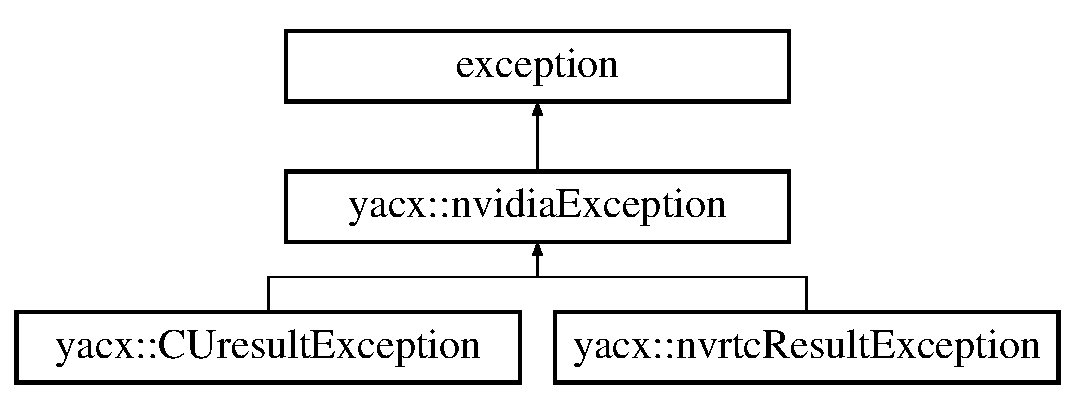
\includegraphics[height=3.000000cm]{classyacx_1_1nvidia_exception}
\end{center}
\end{figure}
\doxysubsection*{Public Member Functions}
\begin{DoxyCompactItemize}
\item 
\mbox{\Hypertarget{classyacx_1_1nvidia_exception_a7fc190c89e3aaac0e5da617fdaf96952}\label{classyacx_1_1nvidia_exception_a7fc190c89e3aaac0e5da617fdaf96952}} 
const char $\ast$ {\bfseries what} () const  throw ()
\end{DoxyCompactItemize}
\doxysubsection*{Protected Attributes}
\begin{DoxyCompactItemize}
\item 
\mbox{\Hypertarget{classyacx_1_1nvidia_exception_a41db782b93c6999a0fd4e6a3b438ae59}\label{classyacx_1_1nvidia_exception_a41db782b93c6999a0fd4e6a3b438ae59}} 
std\+::string {\bfseries error}
\end{DoxyCompactItemize}


\doxysubsection{Detailed Description}
superclass of \mbox{\hyperlink{classyacx_1_1nvrtc_result_exception}{nvrtc\+Result\+Exception}} and cuda\+Result\+Exception 


\begin{DoxyTemplParams}{Template Parameters}
{\em error} & descripton of error \\
\hline
\end{DoxyTemplParams}


The documentation for this class was generated from the following file\+:\begin{DoxyCompactItemize}
\item 
include/yacx/Exception.\+hpp\end{DoxyCompactItemize}

\hypertarget{classyacx_1_1nvrtc_result_exception}{}\section{yacx\+:\+:nvrtc\+Result\+Exception Class Reference}
\label{classyacx_1_1nvrtc_result_exception}\index{yacx\+::nvrtc\+Result\+Exception@{yacx\+::nvrtc\+Result\+Exception}}


Exception class for N\+V\+R\+TC errors.  




{\ttfamily \#include $<$Exception.\+hpp$>$}

Inheritance diagram for yacx\+:\+:nvrtc\+Result\+Exception\+:\begin{figure}[H]
\begin{center}
\leavevmode
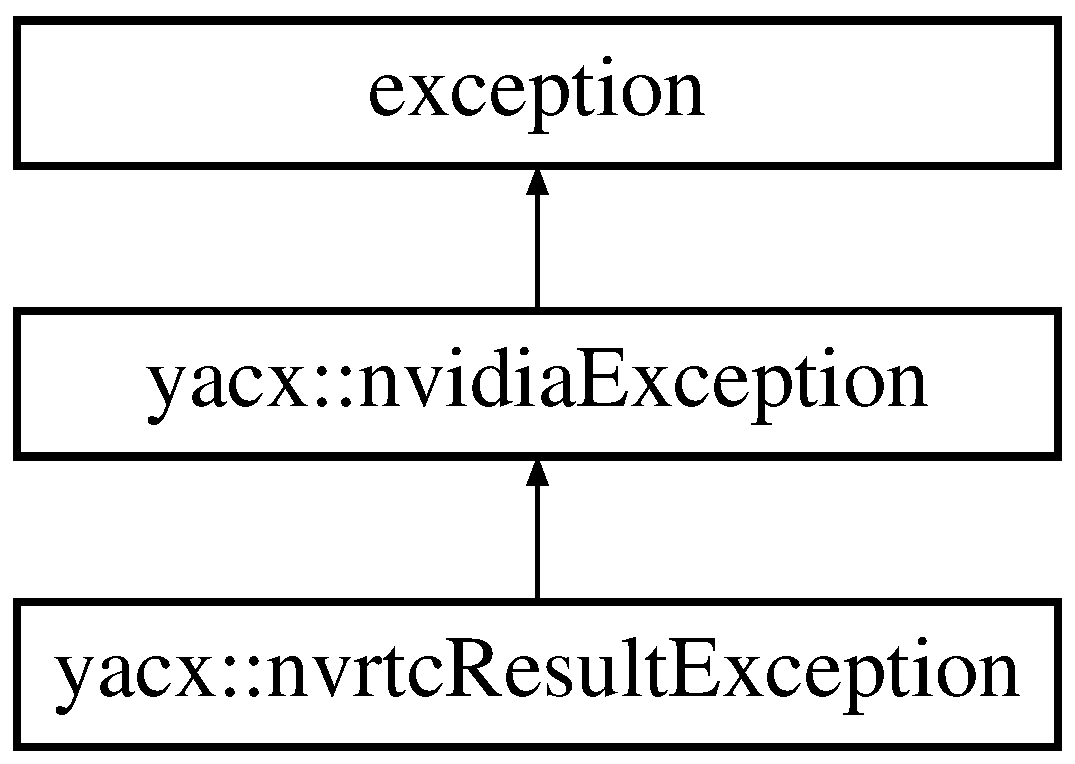
\includegraphics[height=3.000000cm]{classyacx_1_1nvrtc_result_exception}
\end{center}
\end{figure}
\subsection*{Public Member Functions}
\begin{DoxyCompactItemize}
\item 
\mbox{\Hypertarget{classyacx_1_1nvrtc_result_exception_ae054b99ae7de3bb3d2e3b3829a620f6b}\label{classyacx_1_1nvrtc_result_exception_ae054b99ae7de3bb3d2e3b3829a620f6b}} 
{\bfseries nvrtc\+Result\+Exception} (nvrtc\+Result type, std\+::string error)
\end{DoxyCompactItemize}
\subsection*{Public Attributes}
\begin{DoxyCompactItemize}
\item 
\mbox{\Hypertarget{classyacx_1_1nvrtc_result_exception_a613f542dabe2270f6731ff6babfed47e}\label{classyacx_1_1nvrtc_result_exception_a613f542dabe2270f6731ff6babfed47e}} 
nvrtc\+Result {\bfseries type}
\end{DoxyCompactItemize}
\subsection*{Additional Inherited Members}


\subsection{Detailed Description}
Exception class for N\+V\+R\+TC errors. 


\begin{DoxyTemplParams}{Template Parameters}
{\em type} & Name and type of the N\+V\+R\+TC Error, e.\+g. {\ttfamily N\+V\+R\+T\+C\+\_\+\+E\+R\+R\+O\+R\+\_\+\+O\+U\+T\+\_\+\+O\+F\+\_\+\+M\+E\+M\+O\+RY} \\
\hline
{\em error} & description of the N\+V\+R\+TC Error \\
\hline
\end{DoxyTemplParams}
\begin{Desc}
\item[Examples\+: ]\par
\hyperlink{docs_2nvrtcexception_8cpp-example}{docs/nvrtcexception.\+cpp}.\end{Desc}


The documentation for this class was generated from the following file\+:\begin{DoxyCompactItemize}
\item 
include/yacx/Exception.\+hpp\end{DoxyCompactItemize}

\hypertarget{structyacx_1_1detail_1_1opfn}{}\doxysection{yacx\+::detail\+::opfn Struct Reference}
\label{structyacx_1_1detail_1_1opfn}\index{yacx::detail::opfn@{yacx::detail::opfn}}
\doxysubsection*{Public Attributes}
\begin{DoxyCompactItemize}
\item 
\mbox{\Hypertarget{structyacx_1_1detail_1_1opfn_a515ca6f9478e17083fe63dd7e53f57b7}\label{structyacx_1_1detail_1_1opfn_a515ca6f9478e17083fe63dd7e53f57b7}} 
void($\ast$ {\bfseries op} )(void $\ast$$\ast$parameter)
\end{DoxyCompactItemize}


The documentation for this struct was generated from the following file\+:\begin{DoxyCompactItemize}
\item 
include/yacx/cexecutor/Libary\+Loader.\+hpp\end{DoxyCompactItemize}

\hypertarget{classyacx_1_1_options}{}\section{yacx\+:\+:Options Class Reference}
\label{classyacx_1_1_options}\index{yacx\+::\+Options@{yacx\+::\+Options}}


\hyperlink{classyacx_1_1_options}{Options} for compiling a \hyperlink{classyacx_1_1_program}{Program}.  




{\ttfamily \#include $<$Options.\+hpp$>$}

Inheritance diagram for yacx\+:\+:Options\+:\begin{figure}[H]
\begin{center}
\leavevmode
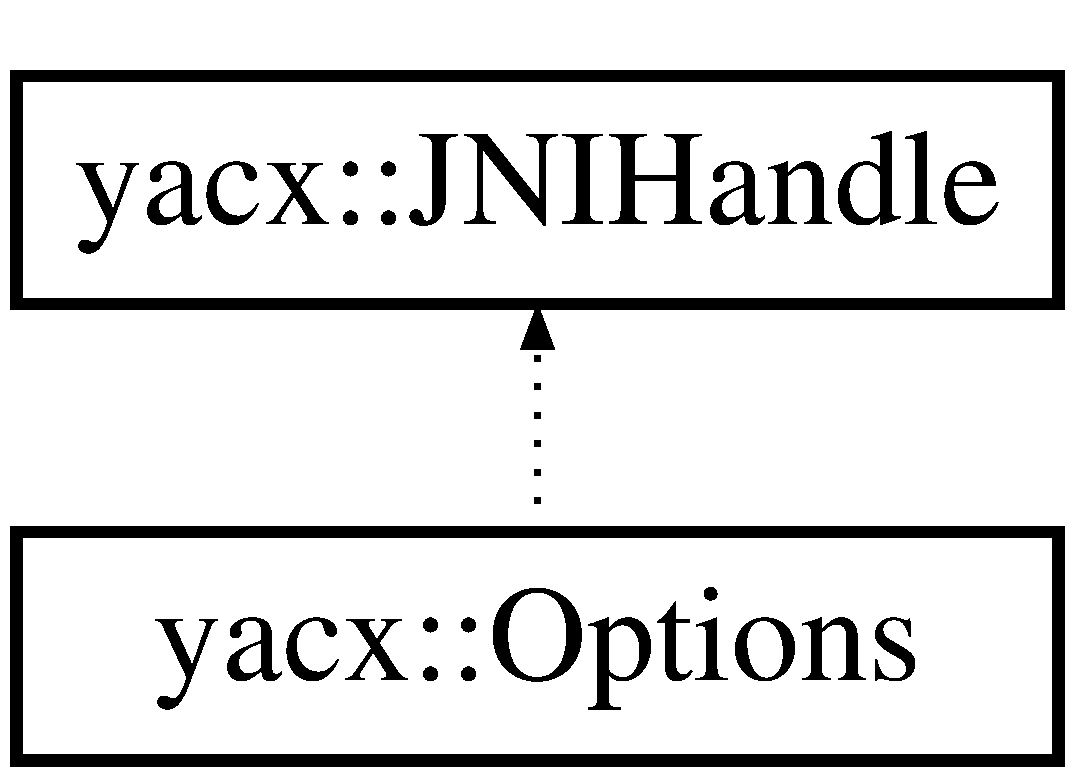
\includegraphics[height=2.000000cm]{classyacx_1_1_options}
\end{center}
\end{figure}
\subsection*{Public Member Functions}
\begin{DoxyCompactItemize}
\item 
\mbox{\Hypertarget{classyacx_1_1_options_aa5138fe978ac803061ced24c9c8134ee}\label{classyacx_1_1_options_aa5138fe978ac803061ced24c9c8134ee}} 
\hyperlink{classyacx_1_1_options_aa5138fe978ac803061ced24c9c8134ee}{Options} ()
\begin{DoxyCompactList}\small\item\em empty \hyperlink{classyacx_1_1_options}{Options} constructor \end{DoxyCompactList}\item 
{\footnotesize template$<$typename T $>$ }\\\hyperlink{classyacx_1_1_options_a73264e0171ac65cdbfb490cdf2b31b58}{Options} (const T \&t)
\item 
{\footnotesize template$<$typename T , typename... TS$>$ }\\\hyperlink{classyacx_1_1_options_a50cf08d2d6c3923123c493df1f0946a7}{Options} (const T \&t, const TS \&... ts)
\item 
void \hyperlink{classyacx_1_1_options_a717bfff574dc2134fae4a0b3ffc9d656}{insert} (const std\+::string \&op)
\item 
void \hyperlink{classyacx_1_1_options_acd9d1aeff97ef155aee30fd3803b0a2a}{insert} (const std\+::string \&name, const std\+::string \&value)
\item 
{\footnotesize template$<$typename T $>$ }\\void \hyperlink{classyacx_1_1_options_a9a8dba0730ac3c5b3bf48bf0889429de}{insert\+Options} (const T \&t)
\item 
{\footnotesize template$<$typename T , typename... TS$>$ }\\void \hyperlink{classyacx_1_1_options_ae24ed09191356cae7c23d55df7f73897}{insert\+Options} (const T \&t, const TS \&... ts)
\item 
const char $\ast$$\ast$ \hyperlink{classyacx_1_1_options_addb823fd1b5f5af2b7c4073bac8ec70b}{content} () const
\item 
auto \hyperlink{classyacx_1_1_options_af68aa0dd2e790d60e75822d8fb7aa4ee}{num\+Options} () const
\end{DoxyCompactItemize}


\subsection{Detailed Description}
\hyperlink{classyacx_1_1_options}{Options} for compiling a \hyperlink{classyacx_1_1_program}{Program}. \begin{Desc}
\item[Examples\+: ]\par
\hyperlink{example_gauss_8cpp-example}{example\+\_\+gauss.\+cpp}, \hyperlink{example_matrix_multiply_8cpp-example}{example\+\_\+matrix\+\_\+multiply.\+cpp}, \hyperlink{example_program_8cpp-example}{example\+\_\+program.\+cpp}, and \hyperlink{example_template_8cpp-example}{example\+\_\+template.\+cpp}.\end{Desc}


\subsection{Constructor \& Destructor Documentation}
\mbox{\Hypertarget{classyacx_1_1_options_a73264e0171ac65cdbfb490cdf2b31b58}\label{classyacx_1_1_options_a73264e0171ac65cdbfb490cdf2b31b58}} 
\index{yacx\+::\+Options@{yacx\+::\+Options}!Options@{Options}}
\index{Options@{Options}!yacx\+::\+Options@{yacx\+::\+Options}}
\subsubsection{\texorpdfstring{Options()}{Options()}\hspace{0.1cm}{\footnotesize\ttfamily [1/2]}}
{\footnotesize\ttfamily template$<$typename T $>$ \\
yacx\+::\+Options\+::\+Options (\begin{DoxyParamCaption}\item[{const T \&}]{t }\end{DoxyParamCaption})}

construct \hyperlink{classyacx_1_1_options}{Options} with one Option 
\begin{DoxyTemplParams}{Template Parameters}
{\em T} & optiontype, e.\+g. F\+M\+AD \\
\hline
\end{DoxyTemplParams}

\begin{DoxyParams}{Parameters}
{\em t} & option \\
\hline
\end{DoxyParams}
\mbox{\Hypertarget{classyacx_1_1_options_a50cf08d2d6c3923123c493df1f0946a7}\label{classyacx_1_1_options_a50cf08d2d6c3923123c493df1f0946a7}} 
\index{yacx\+::\+Options@{yacx\+::\+Options}!Options@{Options}}
\index{Options@{Options}!yacx\+::\+Options@{yacx\+::\+Options}}
\subsubsection{\texorpdfstring{Options()}{Options()}\hspace{0.1cm}{\footnotesize\ttfamily [2/2]}}
{\footnotesize\ttfamily template$<$typename T , typename... TS$>$ \\
yacx\+::\+Options\+::\+Options (\begin{DoxyParamCaption}\item[{const T \&}]{t,  }\item[{const TS \&...}]{ts }\end{DoxyParamCaption})}

construct \hyperlink{classyacx_1_1_options}{Options} with multiple Option 
\begin{DoxyTemplParams}{Template Parameters}
{\em T} & optiontype, e.\+g. F\+M\+AD \\
\hline
{\em TS} & Option \\
\hline
\end{DoxyTemplParams}

\begin{DoxyParams}{Parameters}
{\em t} & optiontype, e.\+g. F\+M\+AD \\
\hline
{\em ts} & Option \\
\hline
\end{DoxyParams}


\subsection{Member Function Documentation}
\mbox{\Hypertarget{classyacx_1_1_options_addb823fd1b5f5af2b7c4073bac8ec70b}\label{classyacx_1_1_options_addb823fd1b5f5af2b7c4073bac8ec70b}} 
\index{yacx\+::\+Options@{yacx\+::\+Options}!content@{content}}
\index{content@{content}!yacx\+::\+Options@{yacx\+::\+Options}}
\subsubsection{\texorpdfstring{content()}{content()}}
{\footnotesize\ttfamily const char $\ast$$\ast$ Options\+::content (\begin{DoxyParamCaption}{ }\end{DoxyParamCaption}) const}

\begin{DoxyReturn}{Returns}
c-\/style string array with all options 
\end{DoxyReturn}
\mbox{\Hypertarget{classyacx_1_1_options_a717bfff574dc2134fae4a0b3ffc9d656}\label{classyacx_1_1_options_a717bfff574dc2134fae4a0b3ffc9d656}} 
\index{yacx\+::\+Options@{yacx\+::\+Options}!insert@{insert}}
\index{insert@{insert}!yacx\+::\+Options@{yacx\+::\+Options}}
\subsubsection{\texorpdfstring{insert()}{insert()}\hspace{0.1cm}{\footnotesize\ttfamily [1/2]}}
{\footnotesize\ttfamily void Options\+::insert (\begin{DoxyParamCaption}\item[{const std\+::string \&}]{op }\end{DoxyParamCaption})}

insert Option 
\begin{DoxyParams}{Parameters}
{\em op} & e.\+g. \char`\"{}-\/-\/device-\/debug\char`\"{} \\
\hline
\end{DoxyParams}
\mbox{\Hypertarget{classyacx_1_1_options_acd9d1aeff97ef155aee30fd3803b0a2a}\label{classyacx_1_1_options_acd9d1aeff97ef155aee30fd3803b0a2a}} 
\index{yacx\+::\+Options@{yacx\+::\+Options}!insert@{insert}}
\index{insert@{insert}!yacx\+::\+Options@{yacx\+::\+Options}}
\subsubsection{\texorpdfstring{insert()}{insert()}\hspace{0.1cm}{\footnotesize\ttfamily [2/2]}}
{\footnotesize\ttfamily void Options\+::insert (\begin{DoxyParamCaption}\item[{const std\+::string \&}]{name,  }\item[{const std\+::string \&}]{value }\end{DoxyParamCaption})}

insert Option 
\begin{DoxyParams}{Parameters}
{\em name} & e.\+g. \char`\"{}-\/-\/fmad\char`\"{} \\
\hline
{\em value} & e.\+g. \char`\"{}false\char`\"{} \\
\hline
\end{DoxyParams}
\mbox{\Hypertarget{classyacx_1_1_options_a9a8dba0730ac3c5b3bf48bf0889429de}\label{classyacx_1_1_options_a9a8dba0730ac3c5b3bf48bf0889429de}} 
\index{yacx\+::\+Options@{yacx\+::\+Options}!insert\+Options@{insert\+Options}}
\index{insert\+Options@{insert\+Options}!yacx\+::\+Options@{yacx\+::\+Options}}
\subsubsection{\texorpdfstring{insert\+Options()}{insertOptions()}\hspace{0.1cm}{\footnotesize\ttfamily [1/2]}}
{\footnotesize\ttfamily template$<$typename T $>$ \\
void yacx\+::\+Options\+::insert\+Options (\begin{DoxyParamCaption}\item[{const T \&}]{t }\end{DoxyParamCaption})}

insert Option 
\begin{DoxyTemplParams}{Template Parameters}
{\em T} & optiontype, e.\+g. F\+M\+AD \\
\hline
\end{DoxyTemplParams}

\begin{DoxyParams}{Parameters}
{\em t} & Option \\
\hline
\end{DoxyParams}
\mbox{\Hypertarget{classyacx_1_1_options_ae24ed09191356cae7c23d55df7f73897}\label{classyacx_1_1_options_ae24ed09191356cae7c23d55df7f73897}} 
\index{yacx\+::\+Options@{yacx\+::\+Options}!insert\+Options@{insert\+Options}}
\index{insert\+Options@{insert\+Options}!yacx\+::\+Options@{yacx\+::\+Options}}
\subsubsection{\texorpdfstring{insert\+Options()}{insertOptions()}\hspace{0.1cm}{\footnotesize\ttfamily [2/2]}}
{\footnotesize\ttfamily template$<$typename T , typename... TS$>$ \\
void yacx\+::\+Options\+::insert\+Options (\begin{DoxyParamCaption}\item[{const T \&}]{t,  }\item[{const TS \&...}]{ts }\end{DoxyParamCaption})}

insert multiple \hyperlink{classyacx_1_1_options}{Options} with multiple Option 
\begin{DoxyTemplParams}{Template Parameters}
{\em T} & optiontype, e.\+g. F\+M\+AD \\
\hline
{\em TS} & Option \\
\hline
\end{DoxyTemplParams}

\begin{DoxyParams}{Parameters}
{\em t} & optiontype, e.\+g. F\+M\+AD \\
\hline
{\em ts} & Option \\
\hline
\end{DoxyParams}
\mbox{\Hypertarget{classyacx_1_1_options_af68aa0dd2e790d60e75822d8fb7aa4ee}\label{classyacx_1_1_options_af68aa0dd2e790d60e75822d8fb7aa4ee}} 
\index{yacx\+::\+Options@{yacx\+::\+Options}!num\+Options@{num\+Options}}
\index{num\+Options@{num\+Options}!yacx\+::\+Options@{yacx\+::\+Options}}
\subsubsection{\texorpdfstring{num\+Options()}{numOptions()}}
{\footnotesize\ttfamily auto yacx\+::\+Options\+::num\+Options (\begin{DoxyParamCaption}{ }\end{DoxyParamCaption}) const\hspace{0.3cm}{\ttfamily [inline]}}

\begin{DoxyReturn}{Returns}
number of \hyperlink{classyacx_1_1_options}{Options} 
\end{DoxyReturn}


The documentation for this class was generated from the following files\+:\begin{DoxyCompactItemize}
\item 
include/yacx/Options.\+hpp\item 
src/Options.\+cpp\end{DoxyCompactItemize}

\hypertarget{classyacx_1_1_program}{}\section{yacx\+:\+:Program Class Reference}
\label{classyacx_1_1_program}\index{yacx\+::\+Program@{yacx\+::\+Program}}


Class to instantiate and compile \hyperlink{classyacx_1_1_source}{Source} (kernel strings)  




{\ttfamily \#include $<$Program.\+hpp$>$}

Inheritance diagram for yacx\+:\+:Program\+:\begin{figure}[H]
\begin{center}
\leavevmode
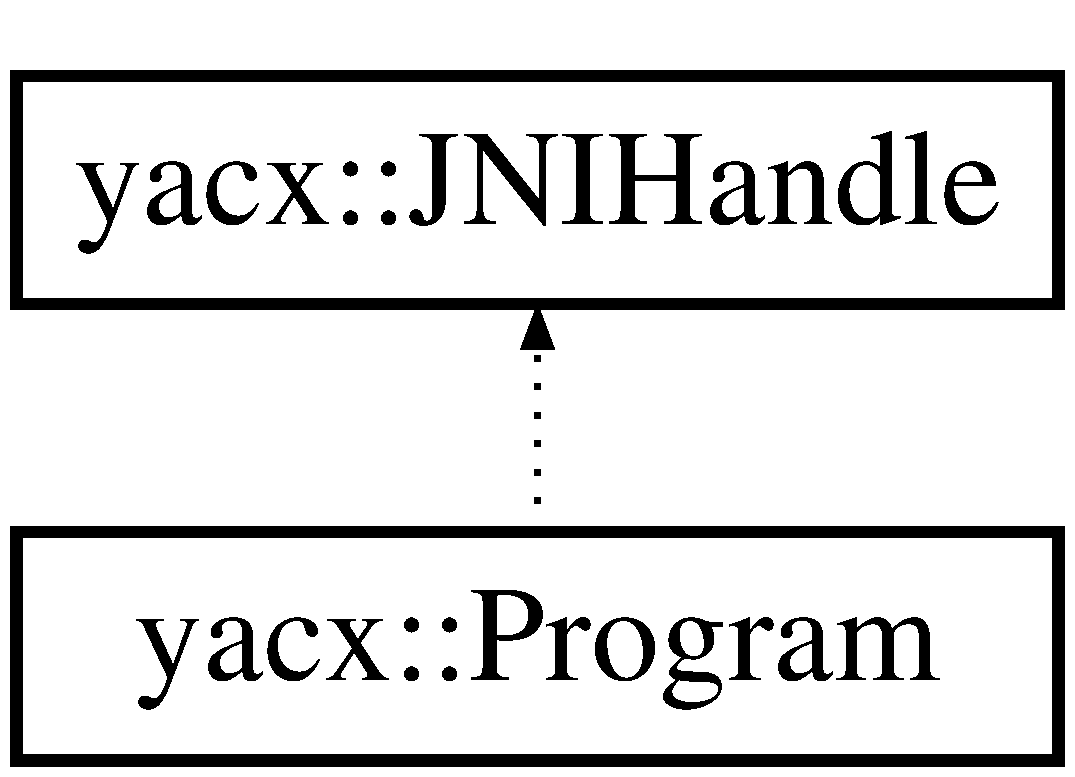
\includegraphics[height=2.000000cm]{classyacx_1_1_program}
\end{center}
\end{figure}
\subsection*{Public Member Functions}
\begin{DoxyCompactItemize}
\item 
\hyperlink{classyacx_1_1_program_a70cf98f664408ede2787e4505365a82a}{Program} (std\+::string kernel\+\_\+name, std\+::shared\+\_\+ptr$<$ nvrtc\+Program $>$ prog)
\item 
{\footnotesize template$<$typename T $>$ }\\\hyperlink{classyacx_1_1_program}{Program} \& \hyperlink{classyacx_1_1_program_a220a1c9deb8d04152e3118530dd79d1f}{instantiate} (T type)
\item 
{\footnotesize template$<$typename T , typename... TS$>$ }\\\hyperlink{classyacx_1_1_program}{Program} \& \hyperlink{classyacx_1_1_program_ad1800bf0daf8b64c357606a26b6e254d}{instantiate} (T type, T\+S... types)
\item 
\hyperlink{classyacx_1_1_kernel}{Kernel} \hyperlink{classyacx_1_1_program_a2834c7f32be3bba037352a5a5e5114d3}{compile} (const \hyperlink{classyacx_1_1_options}{Options} \&options=\hyperlink{classyacx_1_1_options}{Options}())
\item 
std\+::string \hyperlink{classyacx_1_1_program_a0d9e7de768dcbfb251b83737bcaec772}{log} () const
\end{DoxyCompactItemize}


\subsection{Detailed Description}
Class to instantiate and compile \hyperlink{classyacx_1_1_source}{Source} (kernel strings) 

\subsection{Constructor \& Destructor Documentation}
\mbox{\Hypertarget{classyacx_1_1_program_a70cf98f664408ede2787e4505365a82a}\label{classyacx_1_1_program_a70cf98f664408ede2787e4505365a82a}} 
\index{yacx\+::\+Program@{yacx\+::\+Program}!Program@{Program}}
\index{Program@{Program}!yacx\+::\+Program@{yacx\+::\+Program}}
\subsubsection{\texorpdfstring{Program()}{Program()}}
{\footnotesize\ttfamily Program\+::\+Program (\begin{DoxyParamCaption}\item[{std\+::string}]{kernel\+\_\+name,  }\item[{std\+::shared\+\_\+ptr$<$ nvrtc\+Program $>$}]{prog }\end{DoxyParamCaption})}


\begin{DoxyParams}{Parameters}
{\em function\+\_\+name} & function name in kernel string \\
\hline
{\em prog} & \\
\hline
\end{DoxyParams}


\subsection{Member Function Documentation}
\mbox{\Hypertarget{classyacx_1_1_program_a2834c7f32be3bba037352a5a5e5114d3}\label{classyacx_1_1_program_a2834c7f32be3bba037352a5a5e5114d3}} 
\index{yacx\+::\+Program@{yacx\+::\+Program}!compile@{compile}}
\index{compile@{compile}!yacx\+::\+Program@{yacx\+::\+Program}}
\subsubsection{\texorpdfstring{compile()}{compile()}}
{\footnotesize\ttfamily \hyperlink{classyacx_1_1_kernel}{Kernel} Program\+::compile (\begin{DoxyParamCaption}\item[{const \hyperlink{classyacx_1_1_options}{Options} \&}]{options = {\ttfamily \hyperlink{classyacx_1_1_options}{Options}()} }\end{DoxyParamCaption})}

compile \hyperlink{classyacx_1_1_program}{Program} to \hyperlink{classyacx_1_1_kernel}{Kernel} 
\begin{DoxyParams}{Parameters}
{\em options} & see \href{https://docs.nvidia.com/cuda/nvrtc/index.html#group__options}{\tt N\+V\+R\+TC documentation} for supported \hyperlink{classyacx_1_1_options}{Options} \\
\hline
\end{DoxyParams}
\begin{DoxyReturn}{Returns}
a compiled \hyperlink{classyacx_1_1_kernel}{Kernel} 
\end{DoxyReturn}
\mbox{\Hypertarget{classyacx_1_1_program_a220a1c9deb8d04152e3118530dd79d1f}\label{classyacx_1_1_program_a220a1c9deb8d04152e3118530dd79d1f}} 
\index{yacx\+::\+Program@{yacx\+::\+Program}!instantiate@{instantiate}}
\index{instantiate@{instantiate}!yacx\+::\+Program@{yacx\+::\+Program}}
\subsubsection{\texorpdfstring{instantiate()}{instantiate()}\hspace{0.1cm}{\footnotesize\ttfamily [1/2]}}
{\footnotesize\ttfamily template$<$typename T $>$ \\
\hyperlink{classyacx_1_1_program}{Program} \& yacx\+::\+Program\+::instantiate (\begin{DoxyParamCaption}\item[{T}]{type }\end{DoxyParamCaption})}

instantiate template parameter 
\begin{DoxyTemplParams}{Template Parameters}
{\em T} & \\
\hline
\end{DoxyTemplParams}

\begin{DoxyParams}{Parameters}
{\em type} & \\
\hline
\end{DoxyParams}
\begin{DoxyReturn}{Returns}

\end{DoxyReturn}
\mbox{\Hypertarget{classyacx_1_1_program_ad1800bf0daf8b64c357606a26b6e254d}\label{classyacx_1_1_program_ad1800bf0daf8b64c357606a26b6e254d}} 
\index{yacx\+::\+Program@{yacx\+::\+Program}!instantiate@{instantiate}}
\index{instantiate@{instantiate}!yacx\+::\+Program@{yacx\+::\+Program}}
\subsubsection{\texorpdfstring{instantiate()}{instantiate()}\hspace{0.1cm}{\footnotesize\ttfamily [2/2]}}
{\footnotesize\ttfamily template$<$typename T , typename... TS$>$ \\
\hyperlink{classyacx_1_1_program}{Program} \& yacx\+::\+Program\+::instantiate (\begin{DoxyParamCaption}\item[{T}]{type,  }\item[{T\+S...}]{types }\end{DoxyParamCaption})}

instantiate template parameters 
\begin{DoxyTemplParams}{Template Parameters}
{\em T} & \\
\hline
{\em TS} & \\
\hline
\end{DoxyTemplParams}

\begin{DoxyParams}{Parameters}
{\em type} & \\
\hline
{\em types} & \\
\hline
\end{DoxyParams}
\begin{DoxyReturn}{Returns}

\end{DoxyReturn}
\mbox{\Hypertarget{classyacx_1_1_program_a0d9e7de768dcbfb251b83737bcaec772}\label{classyacx_1_1_program_a0d9e7de768dcbfb251b83737bcaec772}} 
\index{yacx\+::\+Program@{yacx\+::\+Program}!log@{log}}
\index{log@{log}!yacx\+::\+Program@{yacx\+::\+Program}}
\subsubsection{\texorpdfstring{log()}{log()}}
{\footnotesize\ttfamily std\+::string yacx\+::\+Program\+::log (\begin{DoxyParamCaption}{ }\end{DoxyParamCaption}) const\hspace{0.3cm}{\ttfamily [inline]}}

\begin{DoxyReturn}{Returns}
log of compilation 
\end{DoxyReturn}


The documentation for this class was generated from the following files\+:\begin{DoxyCompactItemize}
\item 
include/yacx/Program.\+hpp\item 
src/Program.\+cpp\end{DoxyCompactItemize}

\hypertarget{class_program_arg}{}\section{Program\+Arg Class Reference}
\label{class_program_arg}\index{Program\+Arg@{Program\+Arg}}


Class to help launch Kernel with given arguments Arguments are automatically uploaded and downloaded.  




\subsection{Detailed Description}
Class to help launch Kernel with given arguments Arguments are automatically uploaded and downloaded. 

The documentation for this class was generated from the following file\+:\begin{DoxyCompactItemize}
\item 
include/yacx/Kernel\+Args.\+hpp\end{DoxyCompactItemize}

\hypertarget{classyacx_1_1_source}{}\section{yacx\+:\+:Source Class Reference}
\label{classyacx_1_1_source}\index{yacx\+::\+Source@{yacx\+::\+Source}}


Class to wrap kernel strings.  




{\ttfamily \#include $<$Source.\+hpp$>$}

\subsection*{Public Member Functions}
\begin{DoxyCompactItemize}
\item 
\hyperlink{classyacx_1_1_source_ab38b16f1049de5ba1c5c1ccf1a890ece}{Source} (std\+::string kernel\+\_\+string, \hyperlink{classyacx_1_1_headers}{Headers} headers=\hyperlink{classyacx_1_1_headers}{Headers}())
\item 
\hyperlink{classyacx_1_1_program}{Program} \hyperlink{classyacx_1_1_source_a2d95fc130b3c3d6a2a1f20097d5a278f}{program} (const std\+::string \&kernel\+\_\+name)
\end{DoxyCompactItemize}


\subsection{Detailed Description}
Class to wrap kernel strings. \begin{Desc}
\item[Examples\+: ]\par
\hyperlink{docs_2headers_8cpp-example}{docs/headers.\+cpp}, \hyperlink{docs_2kernel_launch_8cpp-example}{docs/kernel\+\_\+launch.\+cpp}, \hyperlink{example_gauss_8cpp-example}{example\+\_\+gauss.\+cpp}, \hyperlink{example_matrix_multiply_8cpp-example}{example\+\_\+matrix\+\_\+multiply.\+cpp}, \hyperlink{example_program_8cpp-example}{example\+\_\+program.\+cpp}, \hyperlink{example_saxpy_8cpp-example}{example\+\_\+saxpy.\+cpp}, and \hyperlink{example_template_8cpp-example}{example\+\_\+template.\+cpp}.\end{Desc}


\subsection{Constructor \& Destructor Documentation}
\mbox{\Hypertarget{classyacx_1_1_source_ab38b16f1049de5ba1c5c1ccf1a890ece}\label{classyacx_1_1_source_ab38b16f1049de5ba1c5c1ccf1a890ece}} 
\index{yacx\+::\+Source@{yacx\+::\+Source}!Source@{Source}}
\index{Source@{Source}!yacx\+::\+Source@{yacx\+::\+Source}}
\subsubsection{\texorpdfstring{Source()}{Source()}}
{\footnotesize\ttfamily Source\+::\+Source (\begin{DoxyParamCaption}\item[{std\+::string}]{kernel\+\_\+string,  }\item[{\hyperlink{classyacx_1_1_headers}{Headers}}]{headers = {\ttfamily \hyperlink{classyacx_1_1_headers}{Headers}()} }\end{DoxyParamCaption})\hspace{0.3cm}{\ttfamily [explicit]}}


\begin{DoxyParams}{Parameters}
{\em kernel\+\_\+string} & \\
\hline
{\em headers} & \hyperlink{classyacx_1_1_headers}{Headers} needed to compile the kernel string \\
\hline
\end{DoxyParams}


\subsection{Member Function Documentation}
\mbox{\Hypertarget{classyacx_1_1_source_a2d95fc130b3c3d6a2a1f20097d5a278f}\label{classyacx_1_1_source_a2d95fc130b3c3d6a2a1f20097d5a278f}} 
\index{yacx\+::\+Source@{yacx\+::\+Source}!program@{program}}
\index{program@{program}!yacx\+::\+Source@{yacx\+::\+Source}}
\subsubsection{\texorpdfstring{program()}{program()}}
{\footnotesize\ttfamily \hyperlink{classyacx_1_1_program}{Program} Source\+::program (\begin{DoxyParamCaption}\item[{const std\+::string \&}]{kernel\+\_\+name }\end{DoxyParamCaption})}

create a \hyperlink{classyacx_1_1_program}{Program} 
\begin{DoxyParams}{Parameters}
{\em function\+\_\+name} & kernel name in kernel string \\
\hline
\end{DoxyParams}
\begin{DoxyReturn}{Returns}
a \hyperlink{classyacx_1_1_program}{Program} 
\end{DoxyReturn}


The documentation for this class was generated from the following files\+:\begin{DoxyCompactItemize}
\item 
include/yacx/Source.\+hpp\item 
src/Source.\+cpp\end{DoxyCompactItemize}

\chapter{File Documentation}
\hypertarget{main_8hpp}{}\section{include/yacx/main.hpp File Reference}
\label{main_8hpp}\index{include/yacx/main.\+hpp@{include/yacx/main.\+hpp}}


C++ bindings to easily compile and execute C\+U\+DA kernels.  


{\ttfamily \#include \char`\"{}yacx/\+Devices.\+hpp\char`\"{}}\newline
{\ttfamily \#include \char`\"{}yacx/\+Exception.\+hpp\char`\"{}}\newline
{\ttfamily \#include \char`\"{}yacx/\+Headers.\+hpp\char`\"{}}\newline
{\ttfamily \#include \char`\"{}yacx/\+Kernel.\+hpp\char`\"{}}\newline
{\ttfamily \#include \char`\"{}yacx/\+Kernel\+Args.\+hpp\char`\"{}}\newline
{\ttfamily \#include \char`\"{}yacx/\+Kernel\+Time.\+hpp\char`\"{}}\newline
{\ttfamily \#include \char`\"{}yacx/\+Logger.\+hpp\char`\"{}}\newline
{\ttfamily \#include \char`\"{}yacx/\+Options.\+hpp\char`\"{}}\newline
{\ttfamily \#include \char`\"{}yacx/\+Program.\+hpp\char`\"{}}\newline
{\ttfamily \#include \char`\"{}yacx/\+Source.\+hpp\char`\"{}}\newline
{\ttfamily \#include \char`\"{}yacx/util.\+hpp\char`\"{}}\newline
{\ttfamily \#include $<$vector\+\_\+types.\+h$>$}\newline


\subsection{Detailed Description}
C++ bindings to easily compile and execute C\+U\+DA kernels. 

\begin{DoxyAuthor}{Author}
Jona Abdinghoff
\end{DoxyAuthor}
\begin{DoxyVersion}{Version}
0.\+6.\+2 
\end{DoxyVersion}

\chapter{Example Documentation}
\hypertarget{_2home_2runner_2work_2yacx_2yacx_2include_2yacx_2_exception_8hpp-example}{}\section{/home/runner/work/yacx/yacx/include/yacx/\+Exception.\+hpp}
docs/cudaexeption.\+cpp


\begin{DoxyCodeInclude}
\textcolor{preprocessor}{#pragma once}

\textcolor{preprocessor}{#include <cstdio>}
\textcolor{preprocessor}{#include <exception>}
\textcolor{preprocessor}{#include <memory>}
\textcolor{preprocessor}{#include <string>}
\textcolor{preprocessor}{#include <vector>}

\textcolor{preprocessor}{#include <cuda.h>}
\textcolor{preprocessor}{#include <nvrtc.h>}
\textcolor{preprocessor}{#include <vector\_types.h>} \textcolor{comment}{// z.B. für dim3}

\textcolor{preprocessor}{#include "yacx/Logger.hpp"} \textcolor{comment}{//um den logger benutzen zu können}

\textcolor{keyword}{namespace }\hyperlink{namespaceyacx}{yacx} \{

\textcolor{keyword}{namespace }detail \{

\textcolor{keywordtype}{unsigned} \textcolor{keywordtype}{int} askTerminalSize();

\textcolor{keyword}{template} <\textcolor{keyword}{class} Container>
\textcolor{keywordtype}{void} split(\textcolor{keyword}{const} std::string &str, Container &cont, \textcolor{keywordtype}{char} delim = \textcolor{charliteral}{' '});

std::string descriptionFkt(\textcolor{keyword}{const} std::string &desc);

std::string whichError(\textcolor{keyword}{const} CUresult &error);

std::string whichError(\textcolor{keyword}{const} nvrtcResult &error);

\} \textcolor{comment}{// namespace detail}

\textcolor{keyword}{class }nvidiaException : \textcolor{keyword}{public} std::exception \{
 \textcolor{keyword}{protected}:
  std::string error;

 \textcolor{keyword}{public}:
  \textcolor{keyword}{const} \textcolor{keywordtype}{char} *what() \textcolor{keyword}{const} \textcolor{keywordflow}{throw}() \{ \textcolor{keywordflow}{return} error.c\_str(); \}
\};

\textcolor{keyword}{class }nvrtcResultException : \textcolor{keyword}{public} nvidiaException \{
 \textcolor{keyword}{public}:
  nvrtcResult type;
  nvrtcResultException(nvrtcResult type, std::string error) \{
    this->type = type;
    this->error = error;
    Logger(loglevel::WARNING)
        << \textcolor{stringliteral}{"nvrtcResultException "} << (int)type
        << \textcolor{stringliteral}{" with description: "} << this->error.c\_str() << \textcolor{stringliteral}{" created."};
  \}
\};

\textcolor{keyword}{class }CUresultException : \textcolor{keyword}{public} nvidiaException \{
 \textcolor{keyword}{public}:
  CUresult type;
  CUresultException(CUresult type, std::string error) \{
    this->type = type;
    this->error = error;
    Logger(loglevel::WARNING)
        << \textcolor{stringliteral}{"CUresultException "} << (int)type
        << \textcolor{stringliteral}{" with description: "} << this->error.c\_str() << \textcolor{stringliteral}{" created."};
  \}
\};

\textcolor{preprocessor}{#define NVRTC\_SAFE\_CALL(error)                                                 \(\backslash\)}
\textcolor{preprocessor}{  \_\_checkNvrtcResultError(error, \_\_FILE\_\_, \_\_LINE\_\_);}
\textcolor{keyword}{inline} \textcolor{keywordtype}{void} \_\_checkNvrtcResultError(\textcolor{keyword}{const} nvrtcResult error, \textcolor{keyword}{const} \textcolor{keywordtype}{char} *file,
                                    \textcolor{keyword}{const} \textcolor{keywordtype}{int} line) \{
  \textcolor{keywordflow}{if} (NVRTC\_SUCCESS != error) \{
    \textcolor{comment}{// create string for exception}
    std::string exception =
        nvrtcGetErrorString(error); \textcolor{comment}{// method to get the error name from NVIDIA}
    exception = exception + \textcolor{stringliteral}{"\(\backslash\)n->occoured in file <"} + file + \textcolor{stringliteral}{" in line "} +
                std::to\_string(line) + \textcolor{stringliteral}{"\(\backslash\)n\(\backslash\)n"};
    \textcolor{keywordflow}{throw} nvrtcResultException(error, exception);
  \}
\}

\textcolor{preprocessor}{#define NVRTC\_SAFE\_CALL\_LOG(error, m\_log)                                      \(\backslash\)}
\textcolor{preprocessor}{  \_\_checkNvrtcResultError\_LOG(error, m\_log, \_\_FILE\_\_, \_\_LINE\_\_);}
\textcolor{keyword}{inline} \textcolor{keywordtype}{void} \_\_checkNvrtcResultError\_LOG(\textcolor{keyword}{const} nvrtcResult error,
                                        std::\_\_cxx11::basic\_string<char> m\_log,
                                        \textcolor{keyword}{const} \textcolor{keywordtype}{char} *file, \textcolor{keyword}{const} \textcolor{keywordtype}{int} line) \{
  \textcolor{keywordflow}{if} (NVRTC\_SUCCESS != error) \{
    \textcolor{comment}{// create string for exception}
    std::string exception =
        nvrtcGetErrorString(error); \textcolor{comment}{// method to get the error name from NVIDIA}
    exception = exception + \textcolor{stringliteral}{"\(\backslash\)n->occoured in file <"} + file + \textcolor{stringliteral}{" in line "} +
                std::to\_string(line) + \textcolor{stringliteral}{"\(\backslash\)n m\_log: "} + m\_log + \textcolor{stringliteral}{"\(\backslash\)n\(\backslash\)n"};
    \textcolor{keywordflow}{throw} nvrtcResultException(error, exception);
  \}
\}

\textcolor{preprocessor}{#define CUDA\_SAFE\_CALL(error)                                                  \(\backslash\)}
\textcolor{preprocessor}{  yacx::\_\_checkCUresultError(error, \_\_FILE\_\_, \_\_LINE\_\_);}
\textcolor{keyword}{inline} \textcolor{keywordtype}{void} \_\_checkCUresultError(\textcolor{keyword}{const} CUresult error, \textcolor{keyword}{const} \textcolor{keywordtype}{char} *file,
                                 \textcolor{keyword}{const} \textcolor{keywordtype}{int} line) \{
  \textcolor{keywordflow}{if} (CUDA\_SUCCESS != error) \{
    \textcolor{comment}{// create string for exception}
    \textcolor{keyword}{const} \textcolor{keywordtype}{char} *name;
    cuGetErrorName(error, &name); \textcolor{comment}{// method to get the error name from NVIDIA}
    \textcolor{keyword}{const} \textcolor{keywordtype}{char} *description;
    cuGetErrorString(
        error, &description); \textcolor{comment}{// method to get the error description from NVIDIA}
    std::string exception = name;
    exception = exception + \textcolor{stringliteral}{"\(\backslash\)n->occoured in file <"} + file + \textcolor{stringliteral}{" in line "} +
                std::to\_string(line) + \textcolor{stringliteral}{"\(\backslash\)n"} + \textcolor{stringliteral}{"  ->"} + description +
                \textcolor{stringliteral}{"\(\backslash\)n"}
                \textcolor{stringliteral}{"  ->"} +
                detail::whichError(error).c\_str() + \textcolor{stringliteral}{"\(\backslash\)n\(\backslash\)n"};
    \textcolor{comment}{// choose which error to throw}
    \textcolor{keywordflow}{throw} CUresultException(error, exception);
  \}
\}

\} \textcolor{comment}{// namespace yacx}
\end{DoxyCodeInclude}
 
\hypertarget{docs_2cudaexeption_8cpp-example}{}\doxysection{docs/cudaexeption.\+cpp}

\begin{DoxyCodeInclude}{0}
\DoxyCodeLine{\textcolor{preprocessor}{\#include "yacx/Exception.hpp"}}
\DoxyCodeLine{}
\DoxyCodeLine{\textcolor{keyword}{using} \mbox{\hyperlink{classyacx_1_1_c_uresult_exception}{yacx::CUresultException}};}
\DoxyCodeLine{}
\DoxyCodeLine{\textcolor{keywordtype}{int} nBytes = 10;}
\DoxyCodeLine{CUdeviceptr d\_A;}
\DoxyCodeLine{\textcolor{keywordflow}{try} \{}
\DoxyCodeLine{  checkCUresultError(cuMemAlloc(\&d\_A, (\textcolor{keywordtype}{unsigned} \textcolor{keywordtype}{int})nBytes));}
\DoxyCodeLine{\} \textcolor{keywordflow}{catch} (CUresultException<(CUresult)1> \&e) \{ \textcolor{comment}{// CUDA\_ERROR\_INVALID\_VALUE}}
\DoxyCodeLine{  std::cout << \textcolor{stringliteral}{"Wrong Exception caught"} << std::endl;}
\DoxyCodeLine{  std::cout << e.what() << std::endl;}
\DoxyCodeLine{\} \textcolor{keywordflow}{catch} (CUresultException<CUDA\_ERROR\_NOT\_INITIALIZED> \&e) \{}
\DoxyCodeLine{  std::cout << \textcolor{stringliteral}{"Correct Exception caught"} << std::endl;}
\DoxyCodeLine{  std::cout << e.what() << std::endl;}
\DoxyCodeLine{\} \textcolor{keywordflow}{catch} (std::exception \&e) \{}
\DoxyCodeLine{  \textcolor{comment}{// Other errors}}
\DoxyCodeLine{  std::cout << \textcolor{stringliteral}{"other Error\(\backslash\)n"};}
\DoxyCodeLine{  std::cout << e.what() << std::endl;}
\DoxyCodeLine{\}}
\end{DoxyCodeInclude}
 
\hypertarget{docs_2headers_8cpp-example}{}\doxysection{docs/headers.\+cpp}

\begin{DoxyCodeInclude}{0}
\DoxyCodeLine{\textcolor{preprocessor}{\#include "yacx/Header.hpp"}}
\DoxyCodeLine{\textcolor{preprocessor}{\#include "yacx/Headers.hpp"}}
\DoxyCodeLine{\textcolor{preprocessor}{\#include "yacx/Source.hpp"}}
\DoxyCodeLine{\textcolor{preprocessor}{\#include "kernels/gauss.h"}}
\DoxyCodeLine{}
\DoxyCodeLine{\textcolor{keyword}{using} \mbox{\hyperlink{classyacx_1_1_source}{yacx::Source}}, \mbox{\hyperlink{classyacx_1_1_headers}{yacx::Headers}}, \mbox{\hyperlink{classyacx_1_1_header}{yacx::Header}};}
\DoxyCodeLine{}
\DoxyCodeLine{Headers headers;}
\DoxyCodeLine{headers.insert(Header\{\textcolor{stringliteral}{"kernels/gauss.h"}\});}
\DoxyCodeLine{Source source\{load(\textcolor{stringliteral}{"kernels/gauss.cu"}), headers\};}
\DoxyCodeLine{}
\DoxyCodeLine{\textcolor{comment}{// Alternatively if you only use one header}}
\DoxyCodeLine{}
\DoxyCodeLine{Source source\{load(\textcolor{stringliteral}{"kernels/gauss.cu"}), Headers\{\textcolor{stringliteral}{"kernels/gauss.h"}\}\};}
\end{DoxyCodeInclude}
 
\hypertarget{docs_2kernel_args_8cpp-example}{}\section{docs/kernel\+\_\+args.\+cpp}
Will execute the Kernel with {\ttfamily add(1, 2, 3, 4, result)}; and the result will be downloaded from device to host


\begin{DoxyCodeInclude}
\textcolor{preprocessor}{#include "yacx/Kernel.hpp"}
\textcolor{preprocessor}{#include "yacx/KernelArgs.hpp"}
\textcolor{preprocessor}{#include "yacx/Program.hpp"}
\textcolor{preprocessor}{#include "yacx/Source.hpp"}

\textcolor{preprocessor}{#include <vector\_types.h>}

\textcolor{keyword}{using} \hyperlink{classyacx_1_1_kernel_arg}{yacx::KernelArg};

\textcolor{keywordtype}{int} a = 1;
\textcolor{keywordtype}{int} b = 2;
\textcolor{keywordtype}{int} c = 3;
\textcolor{keywordtype}{int} d = 4;
\textcolor{keywordtype}{int} result = 0;

std::vector<KernelArg> args;
args.emplace\_back(KernelArg\{&a\});
args.emplace\_back(KernelArg\{&b\});
args.emplace\_back(KernelArg\{&c\});
args.emplace\_back(KernelArg\{&d\});
args.emplace\_back(KernelArg\{&result, \textcolor{keyword}{sizeof}(int), \textcolor{keyword}{true}\});

dim3 grid(1);
dim3 block(1);
source.program(\textcolor{stringliteral}{"add"}).compile().configure(grid, block).launch(args);
\end{DoxyCodeInclude}
 
\hypertarget{docs_2kernel_launch_8cpp-example}{}\section{docs/kernel\+\_\+launch.\+cpp}

\begin{DoxyCodeInclude}
\textcolor{preprocessor}{#include "\hyperlink{main_8hpp}{yacx/main.hpp}"}

\textcolor{keyword}{using} \hyperlink{classyacx_1_1_source}{yacx::Source}, yacx::KernelArg, yacx::Kernel,
    yacx::Device;

Source source\{
    \textcolor{stringliteral}{"extern \(\backslash\)"C\(\backslash\)" \_\_global\_\_\(\backslash\)n"}
    \textcolor{stringliteral}{"void saxpy(float a, float *x, float *y, float *out, size\_t n) \{\(\backslash\)n"}
    \textcolor{stringliteral}{"  size\_t tid = blockIdx.x * blockDim.x + threadIdx.x;\(\backslash\)n"}
    \textcolor{stringliteral}{"  if (tid < n) \{\(\backslash\)n"}
    \textcolor{stringliteral}{"    out[tid] = a * x[tid] + y[tid];\(\backslash\)n"}
    \textcolor{stringliteral}{"  \}\(\backslash\)n"}
    \textcolor{stringliteral}{"\}"}\};

std::vector<KernelArg> args;
args.emplace\_back(KernelArg\{&a\});
args.emplace\_back(KernelArg\{hX.data(), bufferSize\});
args.emplace\_back(KernelArg\{hY.data(), bufferSize\});
args.emplace\_back(KernelArg\{hOut.data(), bufferSize, \textcolor{keyword}{true}, \textcolor{keyword}{false}\});
args.emplace\_back(KernelArg\{&N\});

dim3 grid(NUM\_BLOCKS);
dim3 block(NUM\_THREADS);

Program program = source.program(\textcolor{stringliteral}{"saxpy"});
Kernel kernel = program.compile();
kernel.configure(grid, block);
kernel.launch(args);

\textcolor{comment}{// Alternatively method chaining}

source.program(\textcolor{stringliteral}{"saxpy"})
      .compile()
      .configure(grid, block)
      .launch(args);
\end{DoxyCodeInclude}
 
\hypertarget{docs_2nvrtcexception_8cpp-example}{}\doxysection{docs/nvrtcexception.\+cpp}

\begin{DoxyCodeInclude}{0}
\DoxyCodeLine{\textcolor{preprocessor}{\#include "yacx/Exception.hpp"}}
\DoxyCodeLine{\textcolor{preprocessor}{\#include <nvrtc.h>}}
\DoxyCodeLine{}
\DoxyCodeLine{\textcolor{keyword}{using} \mbox{\hyperlink{classyacx_1_1nvrtc_result_exception}{yacx::nvrtcResultException}};}
\DoxyCodeLine{}
\DoxyCodeLine{\textcolor{keywordflow}{try} \{}
\DoxyCodeLine{  NVRTC\_SAFE\_CALL(nvrtcCompileProgram(\textcolor{keyword}{nullptr}, 0, NULL));}
\DoxyCodeLine{\} \textcolor{keywordflow}{catch} (nvrtcResultException<(nvrtcResult)1> \&e) \{}
\DoxyCodeLine{  std::cout << \textcolor{stringliteral}{"Wrong Exception caught"} << std::endl;}
\DoxyCodeLine{  std::cout << e.what() << std::endl;}
\DoxyCodeLine{\} \textcolor{keywordflow}{catch} (nvrtcResultException<NVRTC\_ERROR\_COMPILATION> \&e) \{}
\DoxyCodeLine{  std::cout << \textcolor{stringliteral}{"Correct Exception caught"} << std::endl;}
\DoxyCodeLine{  std::cout << e.what() << std::endl;}
\DoxyCodeLine{\} \textcolor{keywordflow}{catch} (std::exception \&e) \{}
\DoxyCodeLine{  \textcolor{comment}{// Other errors}}
\DoxyCodeLine{  std::cout << \textcolor{stringliteral}{"other Error\(\backslash\)n"};}
\DoxyCodeLine{  std::cout << e.what() << std::endl;}
\DoxyCodeLine{\}}
\end{DoxyCodeInclude}
 
\hypertarget{docs_2options_construct_8cpp-example}{}\section{docs/options\+\_\+construct.\+cpp}

\begin{DoxyCodeInclude}
\textcolor{preprocessor}{#include "yacx/Device.hpp"}
\textcolor{preprocessor}{#include "yacx/Options.hpp"}

Device device;
Options options\{\hyperlink{classyacx_1_1options_1_1_gpu_architecture}{yacx::options::GpuArchitecture}(device),
                \hyperlink{classyacx_1_1options_1_1_f_m_a_d}{yacx::options::FMAD}(\textcolor{keyword}{false})\};
options.insertOption(\hyperlink{classyacx_1_1options_1_1_fast___math}{yacx::options::Fast\_Math}\{\textcolor{keyword}{true}\});
options.insert(\textcolor{stringliteral}{"--std"}, \textcolor{stringliteral}{"c++14"});
\end{DoxyCodeInclude}
 
\hypertarget{example_gauss_8cpp-example}{}\section{example\+\_\+gauss.\+cpp}

\begin{DoxyCodeInclude}
\textcolor{preprocessor}{#include "kernels/gauss.h"}
\textcolor{preprocessor}{#include "\hyperlink{main_8hpp}{yacx/main.hpp}"}

\textcolor{preprocessor}{#include <cmath>}
\textcolor{preprocessor}{#include <cstdio>}
\textcolor{preprocessor}{#include <fstream>}
\textcolor{preprocessor}{#include <iomanip>}
\textcolor{preprocessor}{#include <iostream>}

\textcolor{preprocessor}{#define NUM\_THREADS 16}
\textcolor{preprocessor}{#define NUM\_BLOCKS 32}

\textcolor{keyword}{using} \hyperlink{classyacx_1_1_source}{yacx::Source}, yacx::KernelArg, yacx::Kernel, yacx::Options, yacx::load,
    yacx::type\_of, yacx::Headers, yacx::Header;

\textcolor{keywordtype}{void} writePPM(Pixel *pixels, \textcolor{keyword}{const} \textcolor{keywordtype}{char} *filename, \textcolor{keywordtype}{int} width, \textcolor{keywordtype}{int} height) \{
  std::ofstream outputFile(filename, std::ios::binary);

  \textcolor{comment}{// write header:}
  outputFile << \textcolor{stringliteral}{"P6\(\backslash\)n"} << width << \textcolor{stringliteral}{" "} << height << \textcolor{stringliteral}{"\(\backslash\)n255\(\backslash\)n"};

  outputFile.write(reinterpret\_cast<const char *>(pixels),
                   \textcolor{keyword}{sizeof}(Pixel) * width * height);
\}

\textcolor{comment}{// Pointer returned must be explicitly freed!}
Pixel *readPPM(\textcolor{keyword}{const} \textcolor{keywordtype}{char} *filename, \textcolor{keywordtype}{int} *width, \textcolor{keywordtype}{int} *height) \{
  std::ifstream inputFile(filename, std::ios::binary);

  \textcolor{comment}{// parse harder}
  \textcolor{comment}{// first line: P6\(\backslash\)n}
  inputFile.ignore(2, \textcolor{charliteral}{'\(\backslash\)n'}); \textcolor{comment}{// ignore P6}
  \textcolor{comment}{// possible comments:}
  \textcolor{keywordflow}{while} (inputFile.peek() == \textcolor{charliteral}{'#'}) \{
    inputFile.ignore(1024, \textcolor{charliteral}{'\(\backslash\)n'});
  \} \textcolor{comment}{// skip comment}
  \textcolor{comment}{// next line: width\_height\(\backslash\)n}
  inputFile >> (*width);
  inputFile.ignore(1, \textcolor{charliteral}{' '}); \textcolor{comment}{// ignore space}
  inputFile >> (*height);
  inputFile.ignore(1, \textcolor{charliteral}{'\(\backslash\)n'}); \textcolor{comment}{// ignore newline}
  \textcolor{comment}{// possible comments:}
  \textcolor{keywordflow}{while} (inputFile.peek() == \textcolor{charliteral}{'#'}) \{
    inputFile.ignore(1024, \textcolor{charliteral}{'\(\backslash\)n'});
  \} \textcolor{comment}{// skip comment}
  \textcolor{comment}{// last header line: 255\(\backslash\)n:}
  inputFile.ignore(3, \textcolor{charliteral}{'\(\backslash\)n'}); \textcolor{comment}{// ignore 255 and newline}

  Pixel *data = \textcolor{keyword}{new} Pixel[(*width) * (*height)];

  inputFile.read(reinterpret\_cast<char *>(data),
                 \textcolor{keyword}{sizeof}(Pixel) * (*width) * (*height));

  \textcolor{keywordflow}{return} data;
\}

\textcolor{keywordtype}{void} calculateWeights(\textcolor{keywordtype}{float} weights[5][5]) \{
  \textcolor{keywordtype}{float} sigma = 1.0;
  \textcolor{keywordtype}{float} r, s = 2.0 * sigma * sigma;

  \textcolor{comment}{// sum is for normalization}
  \textcolor{keywordtype}{float} sum = 0.0;

  \textcolor{comment}{// generate weights for 5x5 kernel}
  \textcolor{keywordflow}{for} (\textcolor{keywordtype}{int} x = -2; x <= 2; x++) \{
    \textcolor{keywordflow}{for} (\textcolor{keywordtype}{int} y = -2; y <= 2; y++) \{
      r = x * x + y * y;
      weights[x + 2][y + 2] = exp(-(r / s)) / (M\_PI * s);
      sum += weights[x + 2][y + 2];
    \}
  \}

  \textcolor{comment}{// normalize the weights}
  \textcolor{keywordflow}{for} (\textcolor{keywordtype}{int} i = 0; i < 5; ++i) \{
    \textcolor{keywordflow}{for} (\textcolor{keywordtype}{int} j = 0; j < 5; ++j) \{
      weights[i][j] /= sum;
    \}
  \}
\}

\textcolor{keywordtype}{int} main(\textcolor{keywordtype}{int} argc, \textcolor{keywordtype}{char} **argv) \{
  \textcolor{keyword}{const} \textcolor{keywordtype}{char} *inFilename = (argc > 1) ? argv[1] : \textcolor{stringliteral}{"kernels/lena.ppm"};
  \textcolor{keyword}{const} \textcolor{keywordtype}{char} *outFilename = (argc > 2) ? argv[2] : \textcolor{stringliteral}{"kernels/output.ppm"};

  \textcolor{keywordtype}{float} weights[5][5];
  calculateWeights(weights);
  \textcolor{keywordtype}{int} width;
  \textcolor{keywordtype}{int} height;

  Pixel *image = readPPM(inFilename, &width, &height);

  \textcolor{keywordflow}{try} \{
    Headers headers;
    headers.insert(Header\{\textcolor{stringliteral}{"kernels/gauss.h"}\});
    Source source\{load(\textcolor{stringliteral}{"kernels/gauss.cu"}), headers\};

    \textcolor{keywordtype}{size\_t} size\_pixel = height * width * \textcolor{keyword}{sizeof}(Pixel);
    \textcolor{keywordtype}{size\_t} size\_weights = 5 * 5 * \textcolor{keyword}{sizeof}(float);

    std::vector<KernelArg> args;
    args.emplace\_back(KernelArg\{image, size\_pixel, \textcolor{keyword}{true}\});
    args.emplace\_back(KernelArg\{weights, size\_weights\});
    args.emplace\_back(KernelArg\{&width\});
    args.emplace\_back(KernelArg\{&height\});

    dim3 block;
    dim3 grid(width, height);
    source.program(\textcolor{stringliteral}{"gaussFilterKernel"})
        .compile()
        .configure(grid, block)
        .launch(args);
  \} \textcolor{keywordflow}{catch} (\textcolor{keyword}{const} std::exception &e) \{
    std::cerr << \textcolor{stringliteral}{"Error:\(\backslash\)n"} << e.what() << std::endl;
  \}

  writePPM(image, outFilename, width, height);
  free(image);

  \textcolor{keywordflow}{return} 0;
\}
\end{DoxyCodeInclude}
 
\hypertarget{example_matrix_multiply_8cpp-example}{}\section{example\+\_\+matrix\+\_\+multiply.\+cpp}

\begin{DoxyCodeInclude}
\textcolor{preprocessor}{#include "\hyperlink{main_8hpp}{yacx/main.hpp}"}

\textcolor{preprocessor}{#include <algorithm>}
\textcolor{preprocessor}{#include <array>}
\textcolor{preprocessor}{#include <cstdio>}
\textcolor{preprocessor}{#include <ctime>}
\textcolor{preprocessor}{#include <functional>}
\textcolor{preprocessor}{#include <iostream>}
\textcolor{preprocessor}{#include <iterator>}
\textcolor{preprocessor}{#include <random>}
\textcolor{preprocessor}{#include <string>}

\textcolor{keyword}{using} \hyperlink{classyacx_1_1_source}{yacx::Source}, yacx::KernelArg, yacx::Kernel, yacx::Options, yacx::Device,
    yacx::load, yacx::KernelTime, yacx::Devices;

\textcolor{keywordtype}{void} compare(\textcolor{keywordtype}{float} *lhs, \textcolor{keywordtype}{float} *rhs, \textcolor{keywordtype}{int} width) \{
  \textcolor{keywordtype}{int} errors = 0;
  \textcolor{keywordflow}{for} (\textcolor{keywordtype}{int} i\{0\}; i < width; i += 1) \{
    \textcolor{comment}{// printf("[%d] expected %f : actually %f\(\backslash\)n", i, lhs[i], rhs[i]);}
    \textcolor{keywordflow}{if} ((lhs[i] - rhs[i]) != 0) \{
      errors += 1;
    \}
  \}
  \textcolor{keywordflow}{if} (errors > 0)
    printf(\textcolor{stringliteral}{"\(\backslash\)u001b[31m%d errors occured, out of %d values.\(\backslash\)u001b[0m\(\backslash\)n"}, errors,
           width);
  \textcolor{keywordflow}{else}
    printf(\textcolor{stringliteral}{"\(\backslash\)u001b[32mno errors occured.\(\backslash\)u001b[0m\(\backslash\)n"});
\}

std::function<bool(const float &, const float &)> comparator =
    [](\textcolor{keyword}{const} \textcolor{keywordtype}{float} &left, \textcolor{keyword}{const} \textcolor{keywordtype}{float} &right) \{
      \textcolor{comment}{// double epsilon\{1.0E-8\};}
      \textcolor{keywordtype}{double} epsilon\{1\};
      \textcolor{keywordflow}{return} (abs(left - right) < epsilon);
    \};

\textcolor{keyword}{template} <\textcolor{keyword}{class} Iter>
\textcolor{keywordtype}{void} fill(Iter start, Iter end, \textcolor{keywordtype}{int} min = 0, \textcolor{keywordtype}{int} max = 100) \{
  \textcolor{keyword}{static} std::random\_device rd;
  \textcolor{keyword}{static} std::mt19937 mte(rd());

  std::uniform\_int\_distribution<int> dist(min, max);

  std::generate(start, end, [&]() \{ \textcolor{keywordflow}{return} dist(mte); \});
\}

\textcolor{keywordtype}{void} MatrixMulSeq(\textcolor{keyword}{const} \textcolor{keywordtype}{float} *M, \textcolor{keyword}{const} \textcolor{keywordtype}{float} *N, \textcolor{keywordtype}{float} *P, \textcolor{keywordtype}{size\_t} width) \{
  \textcolor{keywordtype}{size\_t} Col, Row, k;
  \textcolor{keywordflow}{for} (Col = 0; Col < width; ++Col)
    \textcolor{keywordflow}{for} (Row = 0; Row < width; ++Row) \{
      \textcolor{keywordtype}{float} sum = 0;
      \textcolor{keywordflow}{for} (k = 0; k < width; k += 1) \{
        sum += M[Row * width + k] * N[k * width + Col];
      \}
      P[Row * width + Col] = sum;
    \}
\}

\textcolor{keywordtype}{int} main() \{
  std::clock\_t start;

  \textcolor{keywordtype}{bool} equalMultiply1, equalMultiply1unfolded, equalMultiply2,
      equalMultiplyNaive;

  \textcolor{keyword}{const} \textcolor{keywordtype}{size\_t} WIDTH\{1024\};
  \textcolor{keyword}{const} \textcolor{keywordtype}{size\_t} BLOCK\_SIZE\{16\};
  \textcolor{keyword}{const} \textcolor{keywordtype}{size\_t} GRANULARITY\{4\};
  \textcolor{keyword}{const} \textcolor{keywordtype}{size\_t} matrix\_size\{WIDTH * WIDTH * \textcolor{keyword}{sizeof}(float)\};
  static\_assert(WIDTH % BLOCK\_SIZE == 0);
  static\_assert(BLOCK\_SIZE % GRANULARITY == 0);
  \textcolor{comment}{// problem with WIDTH > 500}
  \textcolor{comment}{// std::array<float, WIDTH * WIDTH> M, N, P\_cuda, P\_seq;}
  \textcolor{keywordtype}{float} *M = \textcolor{keyword}{new} \textcolor{keywordtype}{float}[WIDTH * WIDTH];
  \textcolor{keywordtype}{float} *N = \textcolor{keyword}{new} \textcolor{keywordtype}{float}[WIDTH * WIDTH];
  \textcolor{keywordtype}{float} *P\_seq = \textcolor{keyword}{new} \textcolor{keywordtype}{float}[WIDTH * WIDTH];
  \textcolor{keywordtype}{float} *P\_cuda = \textcolor{keyword}{new} \textcolor{keywordtype}{float}[WIDTH * WIDTH];

  KernelTime time;

  \textcolor{comment}{// Fill arrays with random values}
  \textcolor{comment}{// fill(N.begin(), N.end());}
  \textcolor{comment}{// fill(M.begin(), M.end());}
  fill(M, M + (WIDTH * WIDTH));
  fill(N, N + (WIDTH * WIDTH));

  \textcolor{keywordflow}{try} \{
    \textcolor{comment}{// Select Device}
    Device dev = Devices::findDevice();
    std::cout << \textcolor{stringliteral}{"===================================\(\backslash\)n"};
    std::cout << \textcolor{stringliteral}{"Selected "} << dev.name() << \textcolor{stringliteral}{" with "}
              << (dev.total\_memory() / 1024) / 1024 << \textcolor{stringliteral}{"mb VRAM\(\backslash\)n"};
    std::cout << \textcolor{stringliteral}{"Kernel Arguments total size: "}
              << ((matrix\_size * 3 + \textcolor{keyword}{sizeof}(size\_t)) / 1024) << \textcolor{stringliteral}{"kb\(\backslash\)n\(\backslash\)n"};
    std::cout << \textcolor{stringliteral}{"Theoretical Bandwith:        "}
              << yacx::theoretical\_bandwidth(dev) << \textcolor{stringliteral}{" GB/s\(\backslash\)n"};

    \textcolor{comment}{// Set kernel string and compile options}

    Source source\{load(\textcolor{stringliteral}{"kernels/matrixMult.cu"})\};
    Options options;
    options.insert(\textcolor{stringliteral}{"--std"}, \textcolor{stringliteral}{"c++14"});
    options.insert(\textcolor{stringliteral}{"--device-debug"});
    options.insertOptions(\hyperlink{classyacx_1_1options_1_1_gpu_architecture}{yacx::options::GpuArchitecture}\{dev\});

    \textcolor{comment}{// Set arguments}

    std::vector<KernelArg> args;
    \textcolor{comment}{// args.emplace\_back(KernelArg\{M.data(), matrix\_size\});}
    \textcolor{comment}{// args.emplace\_back(KernelArg\{N.data(), matrix\_size\});}
    \textcolor{comment}{// args.emplace\_back(KernelArg\{P\_cuda.data(), matrix\_size, true, false\});}
    args.emplace\_back(KernelArg\{M, matrix\_size\});
    args.emplace\_back(KernelArg\{N, matrix\_size\});
    args.emplace\_back(KernelArg\{P\_cuda, matrix\_size, \textcolor{keyword}{true}, \textcolor{keyword}{false}\});
    args.emplace\_back(KernelArg\{\textcolor{keyword}{const\_cast<}\textcolor{keywordtype}{size\_t} *\textcolor{keyword}{>}(&WIDTH)\});

    \textcolor{comment}{// Compile Kernels}

    dim3 grid(WIDTH, WIDTH);
    dim3 block(1, 1);
    Kernel kernelNaive = source.program(\textcolor{stringliteral}{"MatrixMultyNaive"})
                             .compile(options)
                             .configure(grid, block);

    block.x = BLOCK\_SIZE;
    block.y = BLOCK\_SIZE / GRANULARITY;
    grid.x = WIDTH / block.x;
    grid.y = WIDTH / GRANULARITY / block.y;
    \textcolor{comment}{//    std::cout << "get\_global\_size(0): " << block.x * grid.x << std::endl;}
    \textcolor{comment}{//    std::cout << "get\_global\_size(1): " << block.y * grid.y << std::endl;}
    \textcolor{comment}{//    std::cout << "get\_local\_size(0): " << block.x << std::endl;}
    \textcolor{comment}{//    std::cout << "get\_local\_size(1): " << block.y << std::endl;}
    Kernel kernel1 = source.program(\textcolor{stringliteral}{"MatrixMulty1"})
                         .instantiate(BLOCK\_SIZE, GRANULARITY)
                         .compile(options)
                         .configure(grid, block);

    block.x = BLOCK\_SIZE;
    block.y = BLOCK\_SIZE / 4;
    grid.x = WIDTH / block.x;
    grid.y = WIDTH / 4 / block.y;
    Kernel kernel1\_1 = source.program(\textcolor{stringliteral}{"MatrixMulty1unfolded"})
                           .instantiate(BLOCK\_SIZE)
                           .compile(options)
                           .configure(grid, block);

    block.x = BLOCK\_SIZE;
    block.y = BLOCK\_SIZE;
    grid.x = WIDTH / BLOCK\_SIZE;
    grid.y = WIDTH / BLOCK\_SIZE;
    Kernel kernel2 = source.program(\textcolor{stringliteral}{"MatrixMulty2"})
                         .instantiate(BLOCK\_SIZE)
                         .compile(options)
                         .configure(grid, block);

    \textcolor{comment}{// Launch kernels}

    \textcolor{comment}{// CPU single threaded matrix multiplication}
    start = std::clock();
    \textcolor{comment}{// MatrixMulSeq(M.data(), N.data(), P\_seq.data(), WIDTH);}
    MatrixMulSeq(M, N, P\_seq, WIDTH);
    std::cout << \textcolor{stringliteral}{"Time"} << yacx::gColorBrightYellow << \textcolor{stringliteral}{"[CPU single threaded]"}
              << yacx::gColorReset << \textcolor{stringliteral}{":   "}
              << (std::clock() - start) / (\textcolor{keywordtype}{double})(CLOCKS\_PER\_SEC / 1000)
              << \textcolor{stringliteral}{" ms"} << std::endl;

    time = kernelNaive.launch(args, dev);
    std::cout << \textcolor{stringliteral}{"Time"} << yacx::gColorBrightYellow << \textcolor{stringliteral}{"[MatrixMultyNaive]"}
              << yacx::gColorReset << \textcolor{stringliteral}{":      "} << time.total << \textcolor{stringliteral}{" ms\(\backslash\)n"};

    std::cout << \textcolor{stringliteral}{"Effective Bandwith:          "}
              << time.effective\_bandwidth\_launch() << \textcolor{stringliteral}{" GB/s\(\backslash\)n"};

    equalMultiplyNaive =
        std::equal(P\_cuda, P\_cuda + (WIDTH * WIDTH), P\_seq, comparator);
    \textcolor{keywordflow}{if} (!equalMultiplyNaive)
      compare(P\_seq, P\_cuda, WIDTH * WIDTH);

    \textcolor{keywordflow}{if} (BLOCK\_SIZE % 4 == 0) \{
      time = kernel1\_1.launch(args, dev);
      std::cout << \textcolor{stringliteral}{"Time"} << yacx::gColorBrightYellow
                << \textcolor{stringliteral}{"[MatrixMulty1unfolded]"} << yacx::gColorReset << \textcolor{stringliteral}{":  "}
                << time.total << \textcolor{stringliteral}{" ms\(\backslash\)n"};

      std::cout << \textcolor{stringliteral}{"Effective Bandwith:          "}
                << time.effective\_bandwidth\_launch() << \textcolor{stringliteral}{" GB/s\(\backslash\)n"};
      equalMultiply1unfolded =
          std::equal(P\_cuda, P\_cuda + (WIDTH * WIDTH), P\_seq, comparator);
      \textcolor{keywordflow}{if} (!equalMultiply1unfolded)
        compare(P\_seq, P\_cuda, WIDTH * WIDTH);
    \} \textcolor{keywordflow}{else} \{
      equalMultiply1unfolded = \textcolor{keyword}{true};
    \}

    time = kernel1.launch(args, dev);
    std::cout << \textcolor{stringliteral}{"Time"} << yacx::gColorBrightYellow << \textcolor{stringliteral}{"[MatrixMulty1]"}
              << yacx::gColorReset << \textcolor{stringliteral}{":          "} << time.total << \textcolor{stringliteral}{" ms\(\backslash\)n"};

    std::cout << \textcolor{stringliteral}{"Effective Bandwith:          "}
              << time.effective\_bandwidth\_launch() << \textcolor{stringliteral}{" GB/s\(\backslash\)n"};
    equalMultiply1 =
        std::equal(P\_cuda, P\_cuda + (WIDTH * WIDTH), P\_seq, comparator);
    \textcolor{keywordflow}{if} (!equalMultiply1)
      compare(P\_seq, P\_cuda, WIDTH * WIDTH);

    time = kernel2.launch(args, dev);
    std::cout << \textcolor{stringliteral}{"Time"} << yacx::gColorBrightYellow << \textcolor{stringliteral}{"[MatrixMulty2]"}
              << yacx::gColorReset << \textcolor{stringliteral}{":          "} << time.total << \textcolor{stringliteral}{" ms\(\backslash\)n"};

    std::cout << \textcolor{stringliteral}{"Effective Bandwith:          "}
              << time.effective\_bandwidth\_launch() << \textcolor{stringliteral}{" GB/s\(\backslash\)n\(\backslash\)n"};
    equalMultiply2 =
        std::equal(P\_cuda, P\_cuda + (WIDTH * WIDTH), P\_seq, comparator);
    \textcolor{keywordflow}{if} (!equalMultiply2)
      compare(P\_seq, P\_cuda, WIDTH * WIDTH);

  \} \textcolor{keywordflow}{catch} (\textcolor{keyword}{const} std::exception &e) \{
    std::cerr << e.what() << std::endl;
    exit(1);
  \}

  \textcolor{keywordflow}{if} (equalMultiplyNaive && equalMultiply1 && equalMultiply1unfolded &&
      equalMultiply2) \{
    std::cout << yacx::gColorBrightGreen
              << \textcolor{stringliteral}{"Everything was correctly calculated!"} << yacx::gColorReset;
  \} \textcolor{keywordflow}{else} \{
    std::cout << yacx::gColorBrightRed;
  \}
  \textcolor{keywordflow}{if} (!equalMultiplyNaive) \{
    std::cout << \textcolor{stringliteral}{"Naive went wrong ;\_;\(\backslash\)n"};
  \}
  \textcolor{keywordflow}{if} (!equalMultiply1) \{
    std::cout << \textcolor{stringliteral}{"Multy1 went wrong ;\_;\(\backslash\)n"};
  \}
  \textcolor{keywordflow}{if} (!equalMultiply1unfolded) \{
    std::cout << \textcolor{stringliteral}{"Multy1unfolded went wrong ;\_;\(\backslash\)n"};
  \}
  \textcolor{keywordflow}{if} (!equalMultiply2) \{
    std::cout << \textcolor{stringliteral}{"Multy2 went wrong ;\_;\(\backslash\)n"};
  \}

  std::cout << yacx::gColorReset
            << \textcolor{stringliteral}{"==================================="} << std::endl;

  \textcolor{comment}{// Free resources}
  \textcolor{keyword}{delete}[] M;
  \textcolor{keyword}{delete}[] N;
  \textcolor{keyword}{delete}[] P\_seq;
  \textcolor{keyword}{delete}[] P\_cuda;

  \textcolor{keywordflow}{return} 0;
\}
\end{DoxyCodeInclude}
 
\hypertarget{example_program_8cpp-example}{}\doxysection{example\+\_\+program.\+cpp}

\begin{DoxyCodeInclude}{0}
\DoxyCodeLine{\textcolor{preprocessor}{\#include "\mbox{\hyperlink{main_8hpp}{yacx/main.hpp}}"}}
\DoxyCodeLine{\textcolor{preprocessor}{\#include <algorithm>}}
\DoxyCodeLine{\textcolor{preprocessor}{\#include <experimental/iterator>}}
\DoxyCodeLine{\textcolor{preprocessor}{\#include <vector>}}
\DoxyCodeLine{}
\DoxyCodeLine{\textcolor{keyword}{using} \mbox{\hyperlink{classyacx_1_1_source}{yacx::Source}}, \mbox{\hyperlink{classyacx_1_1_kernel_arg}{yacx::KernelArg}}, \mbox{\hyperlink{classyacx_1_1_options}{yacx::Options}}, \mbox{\hyperlink{classyacx_1_1_device}{yacx::Device}}, yacx::type\_of,}
\DoxyCodeLine{    \mbox{\hyperlink{classyacx_1_1_devices}{yacx::Devices}};}
\DoxyCodeLine{\textcolor{keywordtype}{int} main(\textcolor{keywordtype}{int} argc, \textcolor{keywordtype}{char} \textcolor{keyword}{const} *\textcolor{keyword}{const} *\textcolor{keyword}{const} argv) \{}
\DoxyCodeLine{  yacx::handle\_logging\_args(argc, argv);}
\DoxyCodeLine{  \textcolor{keyword}{const} \textcolor{keywordtype}{int} data\{1\};}
\DoxyCodeLine{  \textcolor{keyword}{const} \textcolor{keywordtype}{int} times\{4\};}
\DoxyCodeLine{  \textcolor{keyword}{const} \textcolor{keywordtype}{size\_t} size\{32\};}
\DoxyCodeLine{}
\DoxyCodeLine{  static\_assert(!(size \% times));}
\DoxyCodeLine{}
\DoxyCodeLine{  std::vector<int> v;}
\DoxyCodeLine{  v.resize(size);}
\DoxyCodeLine{  std::fill(v.begin(), v.end(), 0);}
\DoxyCodeLine{}
\DoxyCodeLine{  \textcolor{keywordflow}{try} \{}
\DoxyCodeLine{    Device device = Devices::findDevice();}
\DoxyCodeLine{    Options options\{\mbox{\hyperlink{classyacx_1_1options_1_1_gpu_architecture}{yacx::options::GpuArchitecture}}(device),}
\DoxyCodeLine{                    \mbox{\hyperlink{classyacx_1_1options_1_1_f_m_a_d}{yacx::options::FMAD}}(\textcolor{keyword}{false})\};}
\DoxyCodeLine{    options.insert(\textcolor{stringliteral}{"-\/-\/std"}, \textcolor{stringliteral}{"c++14"});}
\DoxyCodeLine{    Source source\{\textcolor{stringliteral}{"template<typename type, int size>\(\backslash\)n"}}
\DoxyCodeLine{                  \textcolor{stringliteral}{"\_\_global\_\_ void my\_kernel(type* c, type val) \{\(\backslash\)n"}}
\DoxyCodeLine{                  \textcolor{stringliteral}{"    auto idx\{blockIdx.x * blockDim.x + threadIdx.x\};\(\backslash\)n"}}
\DoxyCodeLine{                  \textcolor{stringliteral}{"\(\backslash\)n"}}
\DoxyCodeLine{                  \textcolor{stringliteral}{"    \#pragma unroll(size)\(\backslash\)n"}}
\DoxyCodeLine{                  \textcolor{stringliteral}{"    for (auto i\{0\}; i < size; ++i) \{\(\backslash\)n"}}
\DoxyCodeLine{                  \textcolor{stringliteral}{"        c[i] = idx + val;\(\backslash\)n"}}
\DoxyCodeLine{                  \textcolor{stringliteral}{"    \}\(\backslash\)n"}}
\DoxyCodeLine{                  \textcolor{stringliteral}{"\}"}\};}
\DoxyCodeLine{}
\DoxyCodeLine{    std::vector<KernelArg> args;}
\DoxyCodeLine{    args.emplace\_back(KernelArg\{v.data(), \textcolor{keyword}{sizeof}(\textcolor{keywordtype}{int}) * v.size(), \textcolor{keyword}{true}\});}
\DoxyCodeLine{    args.emplace\_back(KernelArg\{\textcolor{keyword}{const\_cast<}\textcolor{keywordtype}{int} *\textcolor{keyword}{>}(\&data)\});}
\DoxyCodeLine{}
\DoxyCodeLine{    dim3 grid(v.size() / times);}
\DoxyCodeLine{    dim3 block(1);}
\DoxyCodeLine{    source.program(\textcolor{stringliteral}{"my\_kernel"})}
\DoxyCodeLine{        .instantiate(type\_of(data), times)}
\DoxyCodeLine{        .compile(options)}
\DoxyCodeLine{        .configure(grid, block)}
\DoxyCodeLine{        .launch(args, device);}
\DoxyCodeLine{  \} \textcolor{keywordflow}{catch} (\textcolor{keyword}{const} std::exception \&e) \{}
\DoxyCodeLine{    std::cerr << e.what() << std::endl;}
\DoxyCodeLine{    exit(1);}
\DoxyCodeLine{  \}}
\DoxyCodeLine{}
\DoxyCodeLine{  std::cout << \textcolor{charliteral}{'\(\backslash\)n'};}
\DoxyCodeLine{  std::copy(v.begin(), v.end(),}
\DoxyCodeLine{            std::experimental::make\_ostream\_joiner(std::cout, \textcolor{stringliteral}{", "}));}
\DoxyCodeLine{  std::cout << std::endl;}
\DoxyCodeLine{}
\DoxyCodeLine{  \textcolor{comment}{// 1, 1, 1, 1, 2, 2, 2, 2, 3, 3, 3, 3, 4, 4, 4, 4, 5, 5, 5, 5, 6, 6, 6, 6, 7,}}
\DoxyCodeLine{  \textcolor{comment}{// 7, 7, 7, 8, 8, 8, 8}}
\DoxyCodeLine{}
\DoxyCodeLine{  \textcolor{keywordflow}{return} 0;}
\DoxyCodeLine{\}}
\end{DoxyCodeInclude}
 
\hypertarget{example_saxpy_8cpp-example}{}\doxysection{example\+\_\+saxpy.\+cpp}

\begin{DoxyCodeInclude}{0}
\DoxyCodeLine{\textcolor{preprocessor}{\#include "\mbox{\hyperlink{main_8hpp}{yacx/main.hpp}}"}}
\DoxyCodeLine{\textcolor{preprocessor}{\#include <stdlib.h>}}
\DoxyCodeLine{}
\DoxyCodeLine{\textcolor{preprocessor}{\#define NUM\_THREADS 512}}
\DoxyCodeLine{\textcolor{preprocessor}{\#define NUM\_BLOCKS 1024}}
\DoxyCodeLine{}
\DoxyCodeLine{\textcolor{keyword}{using} \mbox{\hyperlink{classyacx_1_1_source}{yacx::Source}}, \mbox{\hyperlink{classyacx_1_1_kernel_arg}{yacx::KernelArg}}, \mbox{\hyperlink{structyacx_1_1_kernel_time_struct}{yacx::KernelTime}}, \mbox{\hyperlink{classyacx_1_1_kernel}{yacx::Kernel}},}
\DoxyCodeLine{    \mbox{\hyperlink{classyacx_1_1_device}{yacx::Device}}, \mbox{\hyperlink{classyacx_1_1_devices}{yacx::Devices}}, yacx::load, yacx::type\_of;}
\DoxyCodeLine{}
\DoxyCodeLine{\textcolor{keywordtype}{int} main() \{}
\DoxyCodeLine{  \textcolor{keyword}{const} \textcolor{keywordtype}{float} DELTA\{0.01f\};}
\DoxyCodeLine{  \textcolor{keyword}{const} \textcolor{keywordtype}{size\_t} N\{NUM\_THREADS * NUM\_BLOCKS\};}
\DoxyCodeLine{  \textcolor{keywordtype}{size\_t} bufferSize\{N * \textcolor{keyword}{sizeof}(float)\};}
\DoxyCodeLine{  \textcolor{keywordtype}{float} a\{5.1f\};}
\DoxyCodeLine{  std::array<float, N> hX, hY, hOut;}
\DoxyCodeLine{  \textcolor{keywordflow}{for} (\textcolor{keywordtype}{size\_t} i\{0\}; i < N; ++i) \{}
\DoxyCodeLine{    hX.at(i) = \textcolor{keyword}{static\_cast<}\textcolor{keywordtype}{float}\textcolor{keyword}{>}(i * 0.01);}
\DoxyCodeLine{    hY.at(i) = \textcolor{keyword}{static\_cast<}\textcolor{keywordtype}{float}\textcolor{keyword}{>}(i * 0.02);}
\DoxyCodeLine{  \}}
\DoxyCodeLine{  KernelTime time;}
\DoxyCodeLine{}
\DoxyCodeLine{  \textcolor{keywordflow}{try} \{}
\DoxyCodeLine{    Device dev = Devices::findDevice();}
\DoxyCodeLine{    Source source\{}
\DoxyCodeLine{        \textcolor{stringliteral}{"extern \(\backslash\)"C\(\backslash\)" \_\_global\_\_\(\backslash\)n"}}
\DoxyCodeLine{        \textcolor{stringliteral}{"void saxpy(float a, float *x, float *y, float *out, size\_t n) \{\(\backslash\)n"}}
\DoxyCodeLine{        \textcolor{stringliteral}{"  size\_t tid = blockIdx.x * blockDim.x + threadIdx.x;\(\backslash\)n"}}
\DoxyCodeLine{        \textcolor{stringliteral}{"  if (tid < n) \{\(\backslash\)n"}}
\DoxyCodeLine{        \textcolor{stringliteral}{"    out[tid] = a * x[tid] + y[tid];\(\backslash\)n"}}
\DoxyCodeLine{        \textcolor{stringliteral}{"  \}\(\backslash\)n"}}
\DoxyCodeLine{        \textcolor{stringliteral}{"\}"}\};}
\DoxyCodeLine{}
\DoxyCodeLine{    std::vector<KernelArg> args;}
\DoxyCodeLine{    args.emplace\_back(KernelArg\{\&a\});}
\DoxyCodeLine{    args.emplace\_back(KernelArg\{hX.data(), bufferSize\});}
\DoxyCodeLine{    args.emplace\_back(KernelArg\{hY.data(), bufferSize\});}
\DoxyCodeLine{    args.emplace\_back(KernelArg\{hOut.data(), bufferSize, \textcolor{keyword}{true}, \textcolor{keyword}{false}\});}
\DoxyCodeLine{    args.emplace\_back(KernelArg\{\textcolor{keyword}{const\_cast<}\textcolor{keywordtype}{size\_t} *\textcolor{keyword}{>}(\&N)\});}
\DoxyCodeLine{}
\DoxyCodeLine{    std::cout << \textcolor{stringliteral}{"Selected "} << dev.name() << \textcolor{stringliteral}{" with "}}
\DoxyCodeLine{              << (dev.total\_memory() / 1024) / 1024 << \textcolor{stringliteral}{"mb"} << std::endl;}
\DoxyCodeLine{    std::cout << \textcolor{stringliteral}{"Arguments have a combined size of "}}
\DoxyCodeLine{              << ((bufferSize * 3 + 2 * \textcolor{keyword}{sizeof}(int)) / 1024) << \textcolor{stringliteral}{"kb"}}
\DoxyCodeLine{              << std::endl;}
\DoxyCodeLine{}
\DoxyCodeLine{    dim3 grid(NUM\_BLOCKS);}
\DoxyCodeLine{    dim3 block(NUM\_THREADS);}
\DoxyCodeLine{    time = source.program(\textcolor{stringliteral}{"saxpy"})}
\DoxyCodeLine{               .compile()}
\DoxyCodeLine{               .configure(grid, block)}
\DoxyCodeLine{               .launch(args, dev);}
\DoxyCodeLine{}
\DoxyCodeLine{    std::cout << \textcolor{stringliteral}{"Theoretical Bandwith:        "}}
\DoxyCodeLine{              << yacx::theoretical\_bandwidth(dev) << \textcolor{stringliteral}{" GB/s\(\backslash\)n"};}
\DoxyCodeLine{    std::cout << \textcolor{stringliteral}{"Effective Bandwith:          "}}
\DoxyCodeLine{              << yacx::effective\_bandwidth(time.launch, args.size())}
\DoxyCodeLine{              << \textcolor{stringliteral}{" GB/s\(\backslash\)n"};}
\DoxyCodeLine{  \} \textcolor{keywordflow}{catch} (\textcolor{keyword}{const} std::exception \&e) \{}
\DoxyCodeLine{    std::cerr << \textcolor{stringliteral}{"Error:\(\backslash\)n"} << e.what() << std::endl;}
\DoxyCodeLine{    exit(1);}
\DoxyCodeLine{  \}}
\DoxyCodeLine{}
\DoxyCodeLine{  \textcolor{keywordtype}{bool} correct = \textcolor{keyword}{true};}
\DoxyCodeLine{}
\DoxyCodeLine{  \textcolor{keywordflow}{for} (\textcolor{keywordtype}{size\_t} j = 0; j < hOut.size(); ++j) \{}
\DoxyCodeLine{    \textcolor{keywordtype}{float} expected = hX.at(j) * a + hY.at(j);}
\DoxyCodeLine{    \textcolor{keywordflow}{if} (abs(expected -\/ hOut.at(j)) > DELTA) \{}
\DoxyCodeLine{      correct = \textcolor{keyword}{false};}
\DoxyCodeLine{      std::cout << \textcolor{stringliteral}{"Expected: "} << expected << \textcolor{stringliteral}{" != "}}
\DoxyCodeLine{                << \textcolor{stringliteral}{" Result: "} << hOut.at(j) << std::endl;}
\DoxyCodeLine{    \}}
\DoxyCodeLine{  \}}
\DoxyCodeLine{}
\DoxyCodeLine{  \textcolor{keywordflow}{if} (correct)}
\DoxyCodeLine{    std::cout << \textcolor{stringliteral}{"\(\backslash\)nEverything was correctly calculated!\(\backslash\)n"} << std::endl;}
\DoxyCodeLine{}
\DoxyCodeLine{  std::cout << \textcolor{stringliteral}{"upload time:     "} << time.upload}
\DoxyCodeLine{            << \textcolor{stringliteral}{" ms\(\backslash\)nexecution time:  "} << time.launch}
\DoxyCodeLine{            << \textcolor{stringliteral}{" ms\(\backslash\)ndownload time    "} << time.download}
\DoxyCodeLine{            << \textcolor{stringliteral}{" ms\(\backslash\)ntotal time:      "} << time.total << \textcolor{stringliteral}{" ms.\(\backslash\)n"};}
\DoxyCodeLine{}
\DoxyCodeLine{  std::cout << \textcolor{stringliteral}{"==================================="} << std::endl;}
\DoxyCodeLine{  \textcolor{keywordflow}{return} 0;}
\DoxyCodeLine{\}}
\end{DoxyCodeInclude}
 
\hypertarget{example_template_8cpp-example}{}\section{example\+\_\+template.\+cpp}

\begin{DoxyCodeInclude}
\textcolor{preprocessor}{#include "\hyperlink{main_8hpp}{yacx/main.hpp}"}

\textcolor{keyword}{using} \hyperlink{classyacx_1_1_source}{yacx::Source}, yacx::KernelArg, yacx::Kernel, yacx::Options, yacx::load,
    yacx::type\_of;

\textcolor{keywordtype}{int} main() \{
  \textcolor{keywordtype}{int} result\{\};
  \textcolor{keywordflow}{try} \{
    Source source\{\textcolor{stringliteral}{"template<typename T>\(\backslash\)n"}
                  \textcolor{stringliteral}{"\_\_global\_\_ void f3(int *result) \{ *result = sizeof(T); \}"}\};

    std::vector<KernelArg> args;
    args.push\_back(KernelArg\{&result, \textcolor{keyword}{sizeof}(int), \textcolor{keyword}{true}\});

    dim3 grid(1);
    dim3 block(1);
    source.program(\textcolor{stringliteral}{"f3"})
        .instantiate(\textcolor{stringliteral}{"int"})
        .compile()
        .configure(grid, block)
        .launch(args);
  \} \textcolor{keywordflow}{catch} (\textcolor{keyword}{const} std::exception &e) \{
    std::cerr << e.what() << std::endl;
  \}

  std::cout << \textcolor{stringliteral}{"Expected: "} << \textcolor{keyword}{sizeof}(int) << \textcolor{stringliteral}{" Actual: "} << result
            << std::endl;
  \textcolor{keywordflow}{return} 0;
\}
\end{DoxyCodeInclude}
 
%--- End generated contents ---

% Index
\backmatter
\newpage
\phantomsection
\clearemptydoublepage
\addcontentsline{toc}{chapter}{Index}
\printindex

\end{document}
